% Problems, Chapter 3: Vector Analysis
% Arfken, Weber & Harris, Mathematical Methods for Physicists, 7th ed.
% Requires: amsmath, amssymb, tikz

\section*{Problems}

\Needspace{12\baselineskip}
\subsection*{3.2 Vectors in 3-D Space}

\Needspace{5\baselineskip}
\par\bigskip
\noindent\textbf{3.2.1}\quad If $\mathbf{P}=\hat{\mathbf{e}}_{x}P_{x}
+\hat{\mathbf{e}}_{y}P_{y}$ and $\mathbf{Q}=\hat{\mathbf{e}}_{x}Q_{x}
+\hat{\mathbf{e}}_{y}Q_{y}$ are any two nonparallel (also nonantiparallel)
vectors in the $xy$-plane, show that $\mathbf{P}\times\mathbf{Q}$ is in the
$z$-direction.
\solution
Distribute the cross product, using
$\hat{\mathbf e}_x\times\hat{\mathbf e}_y=\hat{\mathbf e}_z$,
$\hat{\mathbf e}_y\times\hat{\mathbf e}_x=-\hat{\mathbf e}_z$, and
$\hat{\mathbf e}_i\times\hat{\mathbf e}_i=0$:
\[
\begin{aligned}
\mathbf P\times\mathbf Q
&=P_xQ_x(\hat{\mathbf e}_x\times\hat{\mathbf e}_x)
+P_xQ_y(\hat{\mathbf e}_x\times\hat{\mathbf e}_y)
+P_yQ_x(\hat{\mathbf e}_y\times\hat{\mathbf e}_x)
+P_yQ_y(\hat{\mathbf e}_y\times\hat{\mathbf e}_y)\\
&=P_xQ_y\hat{\mathbf e}_z-P_yQ_x\hat{\mathbf e}_z
=\boxed{(P_xQ_y-P_yQ_x)\hat{\mathbf e}_z}.
\end{aligned}
\]
The coefficient is nonzero: its magnitude is
$|\mathbf P\times\mathbf Q|=PQ\sin\theta$, where $\theta$ is the angle
between the vectors, and $\sin\theta\ne0$ because they are neither
parallel ($\theta=0$) nor antiparallel ($\theta=\pi$).
Its sign determines whether the direction is $+z$ or $-z$.

\Needspace{5\baselineskip}
\par\bigskip
\noindent\textbf{3.2.2}\quad Prove that
$(\mathbf{A}\times\mathbf{B})\cdot(\mathbf{A}\times\mathbf{B})
=(AB)^{2}-(\mathbf{A}\cdot\mathbf{B})^{2}$.
\solution
For nonzero $\mathbf A,\mathbf B$, let $\theta$ be their angle.
Then $|\mathbf A\times\mathbf B|=AB\sin\theta$ and
$\mathbf A\cdot\mathbf B=AB\cos\theta$, so
\[
(\mathbf A\times\mathbf B)^2=A^2B^2\sin^2\theta
=A^2B^2(1-\cos^2\theta)
=\boxed{A^2B^2-(\mathbf A\cdot\mathbf B)^2}.
\]
If either vector is zero, both sides are zero directly.
An algebraic check expands both sides in components. The left side is
$(A_yB_z-A_zB_y)^2+(A_zB_x-A_xB_z)^2+(A_xB_y-A_yB_x)^2$;
its squared terms are $\sum_{i\ne j}A_i^2B_j^2$ and its mixed terms
are $-2\sum_{i<j}A_iA_jB_iB_j$. On the right,
\[
A^2B^2=\sum_{i,j}A_i^2B_j^2,\qquad
(\mathbf A\cdot\mathbf B)^2=\sum_iA_i^2B_i^2+2\sum_{i<j}A_iA_jB_iB_j .
\]
In the difference the $i=j$ terms cancel, leaving
$\sum_{i\ne j}A_i^2B_j^2-2\sum_{i<j}A_iA_jB_iB_j$, the same as the
left side.

\Needspace{5\baselineskip}
\par\bigskip
\noindent\textbf{3.2.3}\quad Using the vectors
\[
\begin{split}
\mathbf{P}&=\hat{\mathbf{e}}_{x}\cos\theta+\hat{\mathbf{e}}_{y}\sin\theta,\\
\mathbf{Q}&=\hat{\mathbf{e}}_{x}\cos\varphi-\hat{\mathbf{e}}_{y}\sin\varphi,\\
\mathbf{R}&=\hat{\mathbf{e}}_{x}\cos\varphi+\hat{\mathbf{e}}_{y}\sin\varphi,
\end{split}
\]
prove the familiar trigonometric identities
\[
\sin(\theta+\varphi)=\sin\theta\cos\varphi+\cos\theta\sin\varphi,\quad
\cos(\theta+\varphi)=\cos\theta\cos\varphi-\sin\theta\sin\varphi.
\]
\solution
All three vectors have unit length. Their directed angles from $+x$ are
$\theta,-\varphi,\varphi$, respectively; in particular the directed
angle from $\mathbf Q$ to $\mathbf P$ is $\theta+\varphi$.
Geometrically the dot product and signed $z$-component of the cross
product are
\[
\mathbf Q\cdot\mathbf P=\cos(\theta+\varphi),\qquad
(\mathbf Q\times\mathbf P)_z=\sin(\theta+\varphi).
\]
Here $|\mathbf Q\times\mathbf P|=|\sin(\theta+\varphi)|$, the sine of
the angle between the unit vectors, and by the right-hand rule
$\mathbf Q\times\mathbf P$ points along $+\hat{\mathbf e}_z$ exactly when
the shorter turn from $\mathbf Q$ to $\mathbf P$ is counterclockwise,
i.e.\ when $\sin(\theta+\varphi)>0$; this fixes the sign.
Evaluation from their Cartesian components gives
\[
\mathbf Q\cdot\mathbf P=\cos\varphi\cos\theta-\sin\varphi\sin\theta,
\]
\[
(\mathbf Q\times\mathbf P)_z
=Q_xP_y-Q_yP_x
=\cos\varphi\sin\theta+\sin\varphi\cos\theta.
\]
Equating the geometric and component expressions proves both identities,
including their signs. Directed angles extend the argument to all real
$\theta,\varphi$.
The vector $\mathbf R$ is not needed here. Since its directed angle is
$\varphi$, the same steps give
$\mathbf R\cdot\mathbf P=\cos\varphi\cos\theta+\sin\varphi\sin\theta
=\cos(\theta-\varphi)$ and
$(\mathbf R\times\mathbf P)_z=\cos\varphi\sin\theta-\sin\varphi\cos\theta
=\sin(\theta-\varphi)$, the corresponding difference formulas.

\Needspace{5\baselineskip}
\par\bigskip
\noindent\textbf{3.2.4}\quad
\begin{enumerate}
\item[(a)] Find a vector $\mathbf{A}$ that is perpendicular to
  \[
  \mathbf{U}=2\hat{\mathbf{e}}_{x}+\hat{\mathbf{e}}_{y}-\hat{\mathbf{e}}_{z},
  \quad
  \mathbf{V}=\hat{\mathbf{e}}_{x}-\hat{\mathbf{e}}_{y}+\hat{\mathbf{e}}_{z}.
  \]
\item[(b)] What is $\mathbf{A}$ if, in addition to this requirement, we demand
  that it have unit magnitude?
\end{enumerate}
\solution
\textbf{(a)} Write $\mathbf A=(a,b,c)$. The two perpendicularity
conditions are $2a+b-c=0$ and $a-b+c=0$. Adding gives $3a=0$,
so $a=0$ and then $b=c$. Thus every common perpendicular is
\[
\mathbf A=t(0,1,1).
\]
A nonzero choice is $(0,1,1)$; the cross product
\[
\mathbf U\times\mathbf V
=\bigl(1\cdot1-(-1)(-1),\ (-1)(1)-2\cdot1,\ 2(-1)-1\cdot1\bigr)
=(0,-3,-3)
\]
gives the same direction.
\textbf{(b)} Its squared norm is $2t^2$. Unit magnitude requires
$t=\pm1/\sqrt2$, giving
\[
\boxed{\mathbf A=\pm(\hat{\mathbf e}_y+\hat{\mathbf e}_z)/\sqrt2}.
\]
Both orientations meet the requirements.

\Needspace{5\baselineskip}
\par\bigskip
\noindent\textbf{3.2.5}\quad If four vectors $\mathbf{a}$, $\mathbf{b}$,
$\mathbf{c}$, and $\mathbf{d}$ all lie in the same plane, show that
\[
(\mathbf{a}\times\mathbf{b})\times(\mathbf{c}\times\mathbf{d})=0.
\]
\emph{Hint.}~Consider the directions of the cross-product vectors.
\solution
Let $\hat{\mathbf n}$ be a unit normal to the common plane.
Both $\mathbf a\times\mathbf b$ and $\mathbf c\times\mathbf d$
are normal to it, so they have the forms $\lambda\hat{\mathbf n}$
and $\mu\hat{\mathbf n}$ (including zero if a pair is dependent).
Hence their cross product is
$\lambda\mu(\hat{\mathbf n}\times\hat{\mathbf n})=0$.

\Needspace{5\baselineskip}
\par\bigskip
\noindent\textbf{3.2.6}\quad Derive the law of sines (see Fig.~3.4):
\[
\frac{\sin\alpha}{|A|}=\frac{\sin\beta}{|B|}=\frac{\sin\gamma}{|C|}.
\]
\solution
Take a nondegenerate triangle with side lengths $A,B,C$ opposite
$\alpha,\beta,\gamma$. Its area $\Delta$ is half the magnitude of the
cross product of the two side vectors that leave any one vertex. At the
vertex with angle $\alpha$ these two sides have lengths $B$ and $C$
($A$ is the opposite side), so $2\Delta=BC\sin\alpha$; the other two
vertices are treated the same way:
\[
2\Delta=BC\sin\alpha=CA\sin\beta=AB\sin\gamma.
\]
Divide each expression by the nonzero product $ABC$:
\[
\boxed{\frac{\sin\alpha}{A}=\frac{\sin\beta}{B}
=\frac{\sin\gamma}{C}=\frac{2\Delta}{ABC}}.
\]
This also follows by dropping the altitude from the vertex of angle
$\gamma$ onto the line of side $C$: computed from either of the other
two sides, its length is $h=A\sin\beta=B\sin\alpha$, so
$\sin\alpha/A=\sin\beta/B$. (If $\alpha$ or $\beta$ is obtuse, the foot
lies on the extension of $C$, and the right triangle contains the
supplementary angle, which has the same sine.) The altitude from the
vertex of angle $\alpha$ gives $C\sin\beta=B\sin\gamma$, i.e.\
$\sin\beta/B=\sin\gamma/C$, in the same way.

\Needspace{5\baselineskip}
\par\bigskip
\noindent\textbf{3.2.7}\quad The magnetic induction $\mathbf{B}$ is defined by
the Lorentz force equation,
\[
\mathbf{F}=q(\mathbf{v}\times\mathbf{B}).
\]
Carrying out three experiments, we find that if
\[
\mathbf{v}=\hat{\mathbf{e}}_{x},\quad\frac{\mathbf{F}}{q}
=2\hat{\mathbf{e}}_{z}-4\hat{\mathbf{e}}_{y},
\]
\[
\mathbf{v}=\hat{\mathbf{e}}_{y},\quad\frac{\mathbf{F}}{q}
=4\hat{\mathbf{e}}_{x}-\hat{\mathbf{e}}_{z},
\]
\[
\mathbf{v}=\hat{\mathbf{e}}_{z},\quad\frac{\mathbf{F}}{q}
=\hat{\mathbf{e}}_{y}-2\hat{\mathbf{e}}_{x}.
\]
From the results of these three separate experiments calculate the magnetic
induction $\mathbf{B}$.
\solution
Put $\mathbf B=(B_x,B_y,B_z)$. The three unit-velocity cross products are
\[
\hat{\mathbf e}_x\times\mathbf B=(0,-B_z,B_y),\quad
\hat{\mathbf e}_y\times\mathbf B=(B_z,0,-B_x),\quad
\hat{\mathbf e}_z\times\mathbf B=(-B_y,B_x,0).
\]
Matching components with the measured $\mathbf F/q$: the first
measurement, $(0,-B_z,B_y)=(0,-4,2)$, gives $B_z=4,B_y=2$; the second,
$(B_z,0,-B_x)=(4,0,-1)$, gives $B_z=4,B_x=1$; the third,
$(-B_y,B_x,0)=(-2,1,0)$, independently gives $B_y=2,B_x=1$.
All are consistent, so
$\boxed{\mathbf B=\hat{\mathbf e}_x+2\hat{\mathbf e}_y+4\hat{\mathbf e}_z}$.

\Needspace{5\baselineskip}
\par\bigskip
\noindent\textbf{3.2.8}\quad You are given the three vectors $\mathbf{A}$,
$\mathbf{B}$, and $\mathbf{C}$,
\[
\mathbf{A}=\hat{\mathbf{e}}_{x}+\hat{\mathbf{e}}_{y},\quad
\mathbf{B}=\hat{\mathbf{e}}_{y}+\hat{\mathbf{e}}_{z},\quad
\mathbf{C}=\hat{\mathbf{e}}_{x}-\hat{\mathbf{e}}_{z}.
\]
\begin{enumerate}
\item[(a)] Compute the scalar triple product,
  $\mathbf{A}\cdot\mathbf{B}\times\mathbf{C}$. Noting that
  $\mathbf{A}=\mathbf{B}+\mathbf{C}$, give a geometric interpretation of your
  result for the scalar triple product.
\item[(b)] Compute $\mathbf{A}\times(\mathbf{B}\times\mathbf{C})$.
\end{enumerate}
\solution
First compute, expanding along the first row,
\[
\mathbf B\times\mathbf C
=\begin{vmatrix}\hat{\mathbf e}_x&\hat{\mathbf e}_y&\hat{\mathbf e}_z\\
0&1&1\\1&0&-1\end{vmatrix}
=\hat{\mathbf e}_x(-1-0)-\hat{\mathbf e}_y(0-1)+\hat{\mathbf e}_z(0-1)
=(-1,1,-1).
\]
\textbf{(a)} $\mathbf A\cdot(\mathbf B\times\mathbf C)
=(1,1,0)\cdot(-1,1,-1)=\boxed{0}$.
This is forced by $\mathbf A=\mathbf B+\mathbf C$: since
$\mathbf B\times\mathbf C$ is perpendicular to both $\mathbf B$ and
$\mathbf C$, $(\mathbf B+\mathbf C)\cdot(\mathbf B\times\mathbf C)=0$.
Geometrically, the three vectors lie in one plane, so the
parallelepiped they span has zero volume.
\textbf{(b)} Direct multiplication gives
\[
\mathbf A\times(\mathbf B\times\mathbf C)
=(1,1,0)\times(-1,1,-1)
=\bigl(1(-1)-0\cdot1,\ 0(-1)-1(-1),\ 1\cdot1-1(-1)\bigr)
=\boxed{(-1,1,2)}.
\]
The triple-product identity, with $\mathbf A\cdot\mathbf C=1$ and
$\mathbf A\cdot\mathbf B=1$, also gives
$\mathbf B(\mathbf A\cdot\mathbf C)-\mathbf C(\mathbf A\cdot\mathbf B)
=\mathbf B-\mathbf C=(-1,1,2)$.

\Needspace{5\baselineskip}
\par\bigskip
\noindent\textbf{3.2.9}\quad Prove Jacobi's identity for vector products:
\[
\mathbf{a}\times(\mathbf{b}\times\mathbf{c})
+\mathbf{b}\times(\mathbf{c}\times\mathbf{a})
+\mathbf{c}\times(\mathbf{a}\times\mathbf{b})=0.
\]
\solution
Expand the three vector triple products:
\[
\begin{aligned}
\mathbf a\times(\mathbf b\times\mathbf c)
&=\mathbf b(\mathbf a\cdot\mathbf c)-\mathbf c(\mathbf a\cdot\mathbf b),\\
\mathbf b\times(\mathbf c\times\mathbf a)
&=\mathbf c(\mathbf b\cdot\mathbf a)-\mathbf a(\mathbf b\cdot\mathbf c),\\
\mathbf c\times(\mathbf a\times\mathbf b)
&=\mathbf a(\mathbf c\cdot\mathbf b)-\mathbf b(\mathbf c\cdot\mathbf a).
\end{aligned}
\]
Dot products commute, so the coefficient of each of
$\mathbf a,\mathbf b,\mathbf c$ in the sum is zero. The sum vanishes.

\Needspace{5\baselineskip}
\par\bigskip
\noindent\textbf{3.2.10}\quad A vector $\mathbf{A}$ is decomposed into a
radial vector $\mathbf{A}_{r}$ and a tangential vector $\mathbf{A}_{t}$. If
$\hat{\mathbf{r}}$ is a unit vector in the radial direction, show that
\begin{enumerate}
\item[(a)] $\mathbf{A}_{r}=\hat{\mathbf{r}}(\mathbf{A}\cdot\hat{\mathbf{r}})$
  and
\item[(b)] $\mathbf{A}_{t}=-\hat{\mathbf{r}}\times(\hat{\mathbf{r}}
  \times\mathbf{A})$.
\end{enumerate}
\solution
\textbf{(a)} The radial component must be $\mathbf A_r=a\hat{\mathbf r}$.
The remainder is tangential if
$0=\hat{\mathbf r}\cdot(\mathbf A-a\hat{\mathbf r})
=\hat{\mathbf r}\cdot\mathbf A-a$. Thus
\[
\boxed{\mathbf A_r=\hat{\mathbf r}(\mathbf A\cdot\hat{\mathbf r})}.
\]
\textbf{(b)} The triple-product identity and
$\hat{\mathbf r}\cdot\hat{\mathbf r}=1$ give
\[
-\hat{\mathbf r}\times(\hat{\mathbf r}\times\mathbf A)
=-\bigl[\hat{\mathbf r}(\hat{\mathbf r}\cdot\mathbf A)
-\mathbf A(\hat{\mathbf r}\cdot\hat{\mathbf r})\bigr]
=\mathbf A-\mathbf A_r=\boxed{\mathbf A_t}.
\]
It is perpendicular to $\hat{\mathbf r}$ and the two parts sum to
$\mathbf A$, verifying the decomposition.

\Needspace{5\baselineskip}
\par\bigskip
\noindent\textbf{3.2.11}\quad Prove that a necessary and sufficient condition
for the three (nonvanishing) vectors $\mathbf{A}$, $\mathbf{B}$, and
$\mathbf{C}$ to be coplanar is the vanishing of the scalar triple product
\[
\mathbf{A}\cdot\mathbf{B}\times\mathbf{C}=0.
\]
\solution
If $\mathbf B,\mathbf C$ are independent, their cross product is a
nonzero normal to their plane. Consequently
$\mathbf A\cdot(\mathbf B\times\mathbf C)=0$ says exactly that
$\mathbf A$ lies in that plane. This proves necessity and sufficiency
in this case.
If $\mathbf B,\mathbf C$ are dependent, their cross product is zero, so
the triple product vanishes; and all three vectors lie in a plane
containing $\mathbf A$ and the common line of $\mathbf B,\mathbf C$, so
they are coplanar. Both conditions hold, and again they are equivalent.
Collinear triples are included in this second case.

\Needspace{5\baselineskip}
\par\bigskip
\noindent\textbf{3.2.12}\quad Three vectors $\mathbf{A}$, $\mathbf{B}$, and
$\mathbf{C}$ are given by
\[
\mathbf{A}=3\hat{\mathbf{e}}_{x}-2\hat{\mathbf{e}}_{y}+2\hat{\mathbf{e}}_{z},\quad
\mathbf{B}=6\hat{\mathbf{e}}_{x}+4\hat{\mathbf{e}}_{y}-2\hat{\mathbf{e}}_{z},\quad
\mathbf{C}=-3\hat{\mathbf{e}}_{x}-2\hat{\mathbf{e}}_{y}-4\hat{\mathbf{e}}_{z}.
\]
Compute the values of $\mathbf{A}\cdot\mathbf{B}\times\mathbf{C}$ and
$\mathbf{A}\times(\mathbf{B}\times\mathbf{C})$,
$\mathbf{C}\times(\mathbf{A}\times\mathbf{B})$ and
$\mathbf{B}\times(\mathbf{C}\times\mathbf{A})$.
\solution
The needed cross product, from
$\mathbf B\times\mathbf C=(B_yC_z-B_zC_y,\ B_zC_x-B_xC_z,\ B_xC_y-B_yC_x)$,
and dot products are
\[
\begin{aligned}
\mathbf B\times\mathbf C&=\bigl(4(-4)-(-2)(-2),\ (-2)(-3)-6(-4),\
6(-2)-4(-3)\bigr)=(-20,30,0),\\
\mathbf A\cdot\mathbf B&=18-8-4=6,\\
\mathbf A\cdot\mathbf C&=-9+4-8=-13,\qquad
\mathbf B\cdot\mathbf C=-18-8+8=-18.
\end{aligned}
\]
Therefore the scalar triple product is
\[
\boxed{\mathbf A\cdot(\mathbf B\times\mathbf C)
=3(-20)+(-2)(30)+2(0)=-120}.
\]
Using $\mathbf X\times(\mathbf Y\times\mathbf Z)
=\mathbf Y(\mathbf X\cdot\mathbf Z)-\mathbf Z(\mathbf X\cdot\mathbf Y)$,
\[
\begin{aligned}
\mathbf A\times(\mathbf B\times\mathbf C)
&=\mathbf B(\mathbf A\cdot\mathbf C)-\mathbf C(\mathbf A\cdot\mathbf B)
=-13\mathbf B-6\mathbf C\\
&=(-78+18,\ -52+12,\ 26+24)=\boxed{(-60,-40,50)},\\
\mathbf C\times(\mathbf A\times\mathbf B)
&=\mathbf A(\mathbf C\cdot\mathbf B)-\mathbf B(\mathbf C\cdot\mathbf A)
=-18\mathbf A+13\mathbf B\\
&=(-54+78,\ 36+52,\ -36-26)=\boxed{(24,88,-62)},\\
\mathbf B\times(\mathbf C\times\mathbf A)
&=\mathbf C(\mathbf B\cdot\mathbf A)-\mathbf A(\mathbf B\cdot\mathbf C)
=6\mathbf C+18\mathbf A\\
&=(-18+54,\ -12-36,\ -24+36)=\boxed{(36,-48,12)}.
\end{aligned}
\]
Their sum is $(0,0,0)$, as required by Jacobi's identity
(Exercise 3.2.9).

\Needspace{5\baselineskip}
\par\bigskip
\noindent\textbf{3.2.13}\quad Show that
\[
(\mathbf{A}\times\mathbf{B})\cdot(\mathbf{C}\times\mathbf{D})
=(\mathbf{A}\cdot\mathbf{C})(\mathbf{B}\cdot\mathbf{D})
-(\mathbf{A}\cdot\mathbf{D})(\mathbf{B}\cdot\mathbf{C}).
\]
\solution
Write components using $\varepsilon_{ijk}$, summing every repeated
index from $1$ to $3$. After the cyclic shifts
$\varepsilon_{ijk}=\varepsilon_{jki}$ and
$\varepsilon_{i\ell m}=\varepsilon_{\ell mi}$, the contraction identity
$\sum_k\varepsilon_{ijk}\varepsilon_{pqk}
=\delta_{ip}\delta_{jq}-\delta_{iq}\delta_{jp}$ of Exercise 2.1.9, with
$(i,j,k,p,q)$ renamed $(j,k,i,\ell,m)$, reads
$\varepsilon_{ijk}\varepsilon_{i\ell m}
=\delta_{j\ell}\delta_{km}-\delta_{jm}\delta_{k\ell}$. Hence
\[
\begin{aligned}
(\mathbf A\times\mathbf B)\cdot(\mathbf C\times\mathbf D)
&=\varepsilon_{ijk}\varepsilon_{i\ell m}A_jB_kC_\ell D_m\\
&=(\delta_{j\ell}\delta_{km}-\delta_{jm}\delta_{k\ell})
A_jB_kC_\ell D_m\\
&=\sum_{j,k}A_jC_jB_kD_k-\sum_{j,k}A_jD_jB_kC_k\\
&=(\mathbf A\cdot\mathbf C)(\mathbf B\cdot\mathbf D)
-(\mathbf A\cdot\mathbf D)(\mathbf B\cdot\mathbf C).
\end{aligned}
\]
No independence or nonzero-vector assumption is required.

\Needspace{5\baselineskip}
\par\bigskip
\noindent\textbf{3.2.14}\quad Show that
\[
(\mathbf{A}\times\mathbf{B})\times(\mathbf{C}\times\mathbf{D})
=(\mathbf{A}\cdot\mathbf{B}\times\mathbf{D})\mathbf{C}
-(\mathbf{A}\cdot\mathbf{B}\times\mathbf{C})\mathbf{D}.
\]
\solution
Apply the triple-product identity with $\mathbf X=\mathbf A\times\mathbf B$:
\[
\mathbf X\times(\mathbf C\times\mathbf D)
=\mathbf C(\mathbf X\cdot\mathbf D)-\mathbf D(\mathbf X\cdot\mathbf C).
\]
Cyclicity of the scalar triple product gives
$\mathbf X\cdot\mathbf D=(\mathbf A\times\mathbf B)\cdot\mathbf D
=\mathbf A\cdot(\mathbf B\times\mathbf D)$ and likewise
$\mathbf X\cdot\mathbf C=\mathbf A\cdot(\mathbf B\times\mathbf C)$.
Substituting these two scalars,
\[
(\mathbf A\times\mathbf B)\times(\mathbf C\times\mathbf D)
=\boxed{(\mathbf A\cdot\mathbf B\times\mathbf D)\mathbf C
-(\mathbf A\cdot\mathbf B\times\mathbf C)\mathbf D}.
\]

\Needspace{5\baselineskip}
\par\bigskip
\noindent\textbf{3.2.15}\quad An electric charge $q_{1}$ moving with velocity
$\mathbf{v}_{1}$ produces a magnetic induction $\mathbf{B}$ given by
\[
\mathbf{B}=\frac{\mu_{0}}{4\pi}q_{1}\frac{\mathbf{v}_{1}\times\hat{\mathbf{r}}}
{r^{2}}\quad\text{(mks units)},
\]
where $\hat{\mathbf{r}}$ is a unit vector that points from $q_{1}$ to the
point at which $\mathbf{B}$ is measured (Biot and Savart law).
\begin{enumerate}
\item[(a)] Show that the magnetic force exerted by $q_{1}$ on a second charge
  $q_{2}$, velocity $\mathbf{v}_{2}$, is given by the vector triple product
  \[
  \mathbf{F}_{2}=\frac{\mu_{0}}{4\pi}\frac{q_{1}q_{2}}{r^{2}}\,
  \mathbf{v}_{2}\times(\mathbf{v}_{1}\times\hat{\mathbf{r}}).
  \]
\item[(b)] Write out the corresponding magnetic force $\mathbf{F}_{1}$ that
  $q_{2}$ exerts on $q_{1}$. Define your unit radial vector. How do
  $\mathbf{F}_{1}$ and $\mathbf{F}_{2}$ compare?
\item[(c)] Calculate $\mathbf{F}_{1}$ and $\mathbf{F}_{2}$ for the case of
  $q_{1}$ and $q_{2}$ moving along parallel trajectories side by side.
\end{enumerate}
\par\nobreak\hfill\emph{ANS.}\enspace
(b)\enspace$\mathbf{F}_{1}=-\dfrac{\mu_{0}}{4\pi}\dfrac{q_{1}q_{2}}{r^{2}}\,
\mathbf{v}_{1}\times(\mathbf{v}_{2}\times\hat{\mathbf{r}})$.\enspace
In general, there is no simple relation between $\mathbf{F}_{1}$ and
$\mathbf{F}_{2}$. Specifically, Newton's third law,
$\mathbf{F}_{1}=-\mathbf{F}_{2}$, does not hold.\par
\nobreak\hfill(c)\enspace$\mathbf{F}_{1}=\dfrac{\mu_{0}}{4\pi}
\dfrac{q_{1}q_{2}}{r^{2}}\erratum{(\mathbf v_1\cdot\mathbf v_2)}\hat{\mathbf{r}}=-\mathbf{F}_{2}$.\enspace
\erratum{Mutual attraction if $q_1q_2(\mathbf v_1\cdot\mathbf v_2)>0$; repulsion if it is negative.}
\solution
\textbf{(a)} Set $K=\mu_0q_1q_2/(4\pi r^2)$ and let $\hat{\mathbf r}$
point from charge 1 to charge 2. The field of $q_1$ at $q_2$ is
$\mathbf B_1=(\mu_0/4\pi)q_1\mathbf v_1\times\hat{\mathbf r}/r^2$, so
the magnetic Lorentz force on $q_2$ is
\[
\mathbf F_2=q_2\mathbf v_2\times\mathbf B_1
=K\mathbf v_2\times(\mathbf v_1\times\hat{\mathbf r})
=K\{\mathbf v_1(\mathbf v_2\cdot\hat{\mathbf r})
-\hat{\mathbf r}(\mathbf v_1\cdot\mathbf v_2)\}.
\]
\textbf{(b)} For the field of charge 2 evaluated at charge 1, the unit
vector from the source to the field point is $-\hat{\mathbf r}$, so
$\mathbf B_2=-(\mu_0/4\pi)q_2\mathbf v_2\times\hat{\mathbf r}/r^2$ and
\[
\mathbf F_1=q_1\mathbf v_1\times\mathbf B_2
=-K\mathbf v_1\times(\mathbf v_2\times\hat{\mathbf r})
=K\{\hat{\mathbf r}(\mathbf v_1\cdot\mathbf v_2)
-\mathbf v_2(\mathbf v_1\cdot\hat{\mathbf r})\}.
\]
Thus
$\mathbf F_1+\mathbf F_2
=K[\mathbf v_1(\mathbf v_2\cdot\hat{\mathbf r})
-\mathbf v_2(\mathbf v_1\cdot\hat{\mathbf r})]$, generally nonzero.
For example, if $\mathbf v_1=v\hat{\mathbf r}$ with $v\ne0$ and
$\mathbf v_2\ne0$ is perpendicular to $\hat{\mathbf r}$, then
$\mathbf F_2=0$ (because $\mathbf v_1\times\hat{\mathbf r}=0$), whereas
$\mathbf F_1=-Kv\,\mathbf v_2\ne0$; so $\mathbf F_1\ne-\mathbf F_2$.
This concerns the magnetic forces on the particles; it is not a claim
that particle-plus-field momentum fails to be conserved.

\textbf{(c)} For side-by-side trajectories, both velocities are
perpendicular to $\hat{\mathbf r}$:
$\mathbf v_1\cdot\hat{\mathbf r}=\mathbf v_2\cdot\hat{\mathbf r}=0$.
The first term of $\mathbf F_2$ and the second term of $\mathbf F_1$
then vanish, leaving
\[
\boxed{\mathbf F_1=K(\mathbf v_1\cdot\mathbf v_2)\hat{\mathbf r}
=-\mathbf F_2}.
\]
Because $\hat{\mathbf r}$ points from charge 1 toward charge 2, the
charges attract when $K(\mathbf v_1\cdot\mathbf v_2)>0$.
\erratum{The printed $v^2$ assumes equal velocities.
Attraction requires $q_1q_2(\mathbf v_1\cdot\mathbf v_2)>0$;
opposite sign gives repulsion.}
For equal velocities and like charges this reduces to the printed
attractive result.

\Needspace{12\baselineskip}
\subsection*{3.3 Coordinate Transformations}

\Needspace{5\baselineskip}
\par\bigskip
\noindent\textbf{3.3.1}\quad A rotation $\varphi_{1}+\varphi_{2}$ about the
$z$-axis is carried out as two successive rotations $\varphi_{1}$ and
$\varphi_{2}$, each about the $z$-axis. Use the matrix representation of the
rotations to derive the trigonometric identities
\[
\cos(\varphi_{1}+\varphi_{2})
=\cos\varphi_{1}\cos\varphi_{2}-\sin\varphi_{1}\sin\varphi_{2},\quad
\sin(\varphi_{1}+\varphi_{2})
=\sin\varphi_{1}\cos\varphi_{2}+\cos\varphi_{1}\sin\varphi_{2}.
\]
\solution
For a passive rotation of axes about $z$,
\[
Z(\varphi)=\begin{pmatrix}
\cos\varphi&\sin\varphi&0\\-\sin\varphi&\cos\varphi&0\\0&0&1
\end{pmatrix}.
\]
The two successive rotations give $Z(\varphi_2)Z(\varphi_1)$ (the first
rotation acts first, so its matrix stands on the right).
Multiplying rows of $Z(\varphi_2)$ into columns of $Z(\varphi_1)$, its
upper left block is
\[
\begin{pmatrix}
c_2c_1-s_2s_1&c_2s_1+s_2c_1\\
-s_2c_1-c_2s_1&-s_2s_1+c_2c_1
\end{pmatrix},
\qquad c_i=\cos\varphi_i,\ s_i=\sin\varphi_i;
\]
the third row and column are those of the identity.
Turning the axes through $\varphi_1$ and then through $\varphi_2$ about
the same axis is a single rotation through $\varphi_1+\varphi_2$, so the
product equals $Z(\varphi_1+\varphi_2)$, whose $(1,1)$ and $(1,2)$
entries are $\cos(\varphi_1+\varphi_2)$ and $\sin(\varphi_1+\varphi_2)$.
Equating these entries gives the stated cosine and sine addition
formulas.

\Needspace{5\baselineskip}
\par\bigskip
\noindent\textbf{3.3.2}\quad A corner reflector is formed by three mutually
perpendicular reflecting surfaces. Show that a ray of light incident upon the
corner reflector (striking all three surfaces) is reflected back along a line
parallel to the line of incidence.

\emph{Hint.}~Consider the effect of a reflection on the components of a vector
describing the direction of the light ray.
\solution
Choose $x,y,z$ perpendicular to the three reflecting planes, and let
$\mathbf v=(v_x,v_y,v_z)$ be the propagation direction of the incident
ray.
Reflection reverses the normal component of a ray's direction and
preserves its two tangential components. The three reflection matrices
are therefore
\[
R_x=\operatorname{diag}(-1,1,1),\quad
R_y=\operatorname{diag}(1,-1,1),\quad
R_z=\operatorname{diag}(1,1,-1).
\]
Being diagonal, they commute, and
$R_xR_yR_z=\operatorname{diag}\bigl((-1)(1)(1),\,(1)(-1)(1),\,
(1)(1)(-1)\bigr)=-I_3$. After one reflection from each surface, in any
order, the propagation direction is
$-\mathbf v=(-v_x,-v_y,-v_z)$.
The outgoing line is thus parallel to, and traversed oppositely from,
the incident line; it can be displaced from that line.

\Needspace{5\baselineskip}
\par\bigskip
\noindent\textbf{3.3.3}\quad Let $\mathbf{x}$ and $\mathbf{y}$ be column
vectors. Under an orthogonal transformation $\mathsf{S}$, they become
$\mathbf{x}'=\mathsf{S}\mathbf{x}$ and $\mathbf{y}'=\mathsf{S}\mathbf{y}$.
Show that $(\mathbf{x}')^{T}\mathbf{y}'=\mathbf{x}^{T}\mathbf{y}$, a result
equivalent to the invariance of the dot product under a rotational
transformation.
\solution
Orthogonality means $S^TS=I$. Consequently
\[
(\mathbf x')^T\mathbf y'
=(S\mathbf x)^T(S\mathbf y)
=\mathbf x^TS^TS\mathbf y
=\boxed{\mathbf x^T\mathbf y}.
\]
This argument works for both proper rotations and orthogonal
transformations with determinant $-1$.

\Needspace{5\baselineskip}
\par\bigskip
\noindent\textbf{3.3.4}\quad Given the orthogonal transformation matrix
$\mathsf{S}$ and vectors $\mathbf{a}$ and $\mathbf{b}$,
\[
\mathsf{S}=\begin{pmatrix}0.80&0.60&0.00\\-0.48&0.64&0.60\\
0.36&-0.48&0.80\end{pmatrix},\quad
\mathbf{a}=\begin{pmatrix}1\\0\\1\end{pmatrix},\quad
\mathbf{b}=\begin{pmatrix}0\\2\\-1\end{pmatrix},
\]
\begin{enumerate}
\item[(a)] Calculate $\det(\mathsf{S})$.
\item[(b)] Verify that $\mathbf{a}\cdot\mathbf{b}$ is invariant under
  application of $\mathsf{S}$ to $\mathbf{a}$ and $\mathbf{b}$.
\item[(c)] Determine what happens to $\mathbf{a}\times\mathbf{b}$ under
  application of $\mathsf{S}$ to $\mathbf{a}$ and $\mathbf{b}$. Is this what
  is expected?
\end{enumerate}
\solution
\textbf{(a)} Expansion along the first row ($S_{13}=0$) gives
\[
\begin{aligned}
\det S&=0.80(0.64\cdot0.80+0.60\cdot0.48)
-0.60(-0.48\cdot0.80-0.60\cdot0.36)\\
&=0.80(0.80)-0.60(-0.60)=0.64+0.36=\boxed{1}.
\end{aligned}
\]
\textbf{(b)} Matrix multiplication (each component is a row of $S$
dotted into the column vector) gives
\[
\begin{aligned}
\mathbf a'&=S\mathbf a=(0.80+0.00,\ -0.48+0.60,\ 0.36+0.80)
=(0.80,0.12,1.16),\\
\mathbf b'&=S\mathbf b=\bigl(2(0.60)-0.00,\ 2(0.64)-0.60,\
2(-0.48)-0.80\bigr)=(1.20,0.68,-1.76).
\end{aligned}
\]
Then $\mathbf a\cdot\mathbf b=0+0-1=-1$, and
\[
\mathbf a'\cdot\mathbf b'
=0.80(1.20)+0.12(0.68)+1.16(-1.76)
=0.96+0.0816-2.0416=-1,
\]
so the dot product is invariant.
\textbf{(c)} The original cross product and its transform are
\[
\begin{aligned}
\mathbf a\times\mathbf b
&=(0(-1)-1\cdot2,\ 1\cdot0-1(-1),\ 1\cdot2-0\cdot0)=(-2,1,2),\\
S(\mathbf a\times\mathbf b)
&=(-1.60+0.60+0,\ 0.96+0.64+1.20,\ -0.72-0.48+1.60)
=(-1.00,2.80,0.40).
\end{aligned}
\]
The cross product after transformation is
\[
\begin{aligned}
\mathbf a'\times\mathbf b'
&=(0.12(-1.76)-1.16(0.68),\
1.16(1.20)-0.80(-1.76),\
0.80(0.68)-0.12(1.20))\\
&=(-0.2112-0.7888,\ 1.392+1.408,\ 0.544-0.144)
=(-1.00,2.80,0.40).
\end{aligned}
\]
This is expected: the cross product of two vectors is a pseudovector
(Section 3.3), i.e.\ for orthogonal $S$,
$(S\mathbf a)\times(S\mathbf b)=(\det S)S(\mathbf a\times\mathbf b)$,
and here $\det S=1$.
To verify this law, note that
$\sum_{ijk}\varepsilon_{ijk}S_{i\ell}S_{jm}S_{kn}$ is the determinant of
the matrix whose columns are columns $\ell,m,n$ of $S$, which is
$(\det S)\varepsilon_{\ell mn}$: it vanishes when two columns coincide
and changes sign under each interchange of columns. Hence
\[
\bigl(S^T[(S\mathbf a)\times(S\mathbf b)]\bigr)_\ell
=\sum_{ijkmn}\varepsilon_{ijk}S_{i\ell}S_{jm}S_{kn}a_mb_n
=(\det S)(\mathbf a\times\mathbf b)_\ell ,
\]
and multiplying by $S$, with $SS^T=I$, gives the law.

\Needspace{5\baselineskip}
\par\bigskip
\noindent\textbf{3.3.5}\quad Using $\mathbf{a}$ and $\mathbf{b}$ as defined in
Exercise 3.3.4, but with
\[
\mathsf{S}=\begin{pmatrix}0.60&0.00&0.80\\-0.64&-0.60&0.48\\
-0.48&0.80&0.36\end{pmatrix}\quad\text{and}\quad
\mathbf{c}=\begin{pmatrix}2\\1\\3\end{pmatrix},
\]
\begin{enumerate}
\item[(a)] Calculate $\det(\mathsf{S})$.

  Apply $\mathsf{S}$ to $\mathbf{a}$, $\mathbf{b}$, and $\mathbf{c}$, and
  determine what happens to
\item[(b)] $\mathbf{a}\times\mathbf{b}$,
\item[(c)] $(\mathbf{a}\times\mathbf{b})\cdot\mathbf{c}$,
\item[(d)] $\mathbf{a}\times(\mathbf{b}\times\mathbf{c})$.
\item[(e)] Classify the expressions in (b) through (d) as scalar, vector,
  pseudovector, or pseudoscalar.
\end{enumerate}
\solution
\textbf{(a)} Expansion along the first row, whose middle entry is zero,
gives
\[
\begin{aligned}
\det S&=0.60(-0.60\cdot0.36-0.48\cdot0.80)
+0.80(-0.64\cdot0.80-(-0.60)(-0.48))\\
&=0.60(-0.60)+0.80(-0.80)=-0.36-0.64=\boxed{-1}.
\end{aligned}
\]
Multiplying $S$ into the three column vectors gives
\[
\begin{aligned}
\mathbf a'&=(0.60+0.80,\ -0.64+0.48,\ -0.48+0.36)=(1.40,-0.16,-0.12),\\
\mathbf b'&=(0-0.80,\ -1.20-0.48,\ 1.60-0.36)=(-0.80,-1.68,1.24),\\
\mathbf c'&=(1.20+0+2.40,\ -1.28-0.60+1.44,\ -0.96+0.80+1.08)
=(3.60,-0.44,0.92).
\end{aligned}
\]
\textbf{(b)} With $\mathbf a\times\mathbf b=(-2,1,2)$ from
Exercise 3.3.4,
\[
S(\mathbf a\times\mathbf b)
=(-1.20+0+1.60,\ 1.28-0.60+0.96,\ 0.96+0.80+0.72)=(0.40,1.64,2.48),
\]
whereas
\[
\begin{aligned}
\mathbf a'\times\mathbf b'
&=\bigl((-0.16)(1.24)-(-0.12)(-1.68),\
(-0.12)(-0.80)-1.40(1.24),\\
&\qquad 1.40(-1.68)-(-0.16)(-0.80)\bigr)\\
&=(-0.1984-0.2016,\ 0.096-1.736,\ -2.352-0.128)\\
&=(-0.40,-1.64,-2.48)=-S(\mathbf a\times\mathbf b).
\end{aligned}
\]
\textbf{(c)} The original triple product is
$(-2,1,2)\cdot(2,1,3)=-4+1+6=3$; the new one is
\[
(\mathbf a'\times\mathbf b')\cdot\mathbf c'
=(-0.40)(3.60)+(-1.64)(-0.44)+(-2.48)(0.92)
=-1.44+0.7216-2.2816=-3.
\]
\textbf{(d)} Since $\mathbf a\cdot\mathbf c=2+0+3=5$ and
$\mathbf a\cdot\mathbf b=-1$,
\[
\mathbf a\times(\mathbf b\times\mathbf c)
=\mathbf b(\mathbf a\cdot\mathbf c)-\mathbf c(\mathbf a\cdot\mathbf b)
=5\mathbf b+\mathbf c=(0,10,-5)+(2,1,3)=(2,11,-2).
\]
Dot products are unchanged by any orthogonal $S$ (Exercise 3.3.3), so
the same identity gives for the transformed vectors
\[
\begin{aligned}
\mathbf a'\times(\mathbf b'\times\mathbf c')
&=5\mathbf b'+\mathbf c'
=(-4.00+3.60,\ -8.40-0.44,\ 6.20+0.92)\\
&=(-0.40,-8.84,7.12)=S(2,11,-2),
\end{aligned}
\]
since $S(2,11,-2)=(1.20+0-1.60,\ -1.28-6.60-0.96,\ -0.96+8.80-0.72)$.
\textbf{(e)} Thus (b) is a pseudovector, (c) a pseudoscalar, and
(d) an ordinary vector. A pseudovector acquires the extra factor
$\det S$, and a pseudoscalar changes sign under this improper rotation.

\erratum{The Instructor's Manual, p.~36, prints $S_{32}=-0.80$ in its
matrices; the textbook has $+0.80$, as used here. With $+0.80$ the rows
of $S$ are orthonormal; with $-0.80$ the second and third rows would
have scalar product $(-0.64)(-0.48)+(-0.60)(-0.80)+0.48(0.36)=0.96\ne0$,
so $S$ would not be orthogonal. The transformed vectors listed in the
Instructor's Manual also require the positive sign. For example,
$b'_z=0.80(2)+0.36(-1)=1.24$, whereas the negative sign gives $-1.96$.}

\Needspace{12\baselineskip}
\subsection*{3.4 Rotations in \texorpdfstring{$\mathbb{R}^{3}$}{R3}}

\Needspace{5\baselineskip}
\par\bigskip
\noindent\textbf{3.4.1}\quad Another set of Euler rotations in common use is
\begin{enumerate}
\item[(1)] a rotation about the $x_{3}$-axis through an angle $\varphi$,
  counterclockwise,
\item[(2)] a rotation about the $x'_{1}$-axis through an angle $\theta$,
  counterclockwise,
\item[(3)] a rotation about the $x''_{3}$-axis through an angle $\psi$,
  counterclockwise.
\end{enumerate}
If
\[
\begin{alignedat}{3}
\alpha&=\varphi-\pi/2&\qquad\varphi&=\alpha+\pi/2\\
\beta&=\theta&\text{or}\qquad\theta&=\beta\\
\gamma&=\psi+\pi/2&\psi&=\gamma-\pi/2,
\end{alignedat}
\]
show that the final systems are identical.
\solution
Use passive rotation matrices
\[
Z(t)=\begin{pmatrix}c_t&s_t&0\\-s_t&c_t&0\\0&0&1\end{pmatrix},\
Y(t)=\begin{pmatrix}c_t&0&-s_t\\0&1&0\\s_t&0&c_t\end{pmatrix},\
X(t)=\begin{pmatrix}1&0&0\\0&c_t&s_t\\0&-s_t&c_t\end{pmatrix},
\]
where $c_t=\cos t,s_t=\sin t$.
The textbook convention (rotations about $x_3$, $x'_2$, $x''_3$, each
later rotation multiplying from the left) is
$S(\alpha,\beta,\gamma)=Z(\gamma)Y(\beta)Z(\alpha)$.
The alternative set, whose second rotation is about $x'_1$, is likewise
$Z(\psi)X(\theta)Z(\varphi)$.
For the quarter turns, $c_{\pm\pi/2}=0$ and $s_{\pm\pi/2}=\pm1$, so
\[
Z(-\pi/2)=\begin{pmatrix}0&-1&0\\1&0&0\\0&0&1\end{pmatrix},\qquad
Z(\pi/2)=\begin{pmatrix}0&1&0\\-1&0&0\\0&0&1\end{pmatrix}.
\]
Multiplying $Y(\theta)$ on the right by $Z(-\pi/2)$ replaces its
columns $(\mathbf k_1,\mathbf k_2,\mathbf k_3)$ by
$(\mathbf k_2,-\mathbf k_1,\mathbf k_3)$:
\[
Y(\theta)Z(-\pi/2)
=\begin{pmatrix}0&-c_\theta&-s_\theta\\1&0&0\\0&-s_\theta&c_\theta
\end{pmatrix},
\]
and multiplying on the left by $Z(\pi/2)$ replaces the rows
$(\mathbf r_1,\mathbf r_2,\mathbf r_3)$ of this matrix by
$(\mathbf r_2,-\mathbf r_1,\mathbf r_3)$:
\[
Z(\pi/2)Y(\theta)Z(-\pi/2)
=\begin{pmatrix}1&0&0\\0&c_\theta&s_\theta\\0&-s_\theta&c_\theta\end{pmatrix}
=X(\theta).
\]
Consequently, under the stated substitutions, and with
$Z(a+b)=Z(a)Z(b)=Z(b)Z(a)$ (Exercise 3.3.1),
\[
\begin{aligned}
S&=Z(\psi+\pi/2)Y(\theta)Z(\varphi-\pi/2)\\
&=Z(\psi)\,[Z(\pi/2)Y(\theta)Z(-\pi/2)]\,Z(\varphi)
=Z(\psi)X(\theta)Z(\varphi).
\end{aligned}
\]
The matrices, and therefore the final frames, coincide.
For use below, the explicit product $Z(\gamma)Y(\beta)Z(\alpha)$, the
textbook's Eq.~(3.37), is
\begin{equation}\tag{3.37}\label{ch03:euler}
S=\begin{pmatrix}
c_\gamma c_\beta c_\alpha-s_\gamma s_\alpha&
c_\gamma c_\beta s_\alpha+s_\gamma c_\alpha&-c_\gamma s_\beta\\
-s_\gamma c_\beta c_\alpha-c_\gamma s_\alpha&
-s_\gamma c_\beta s_\alpha+c_\gamma c_\alpha&s_\gamma s_\beta\\
s_\beta c_\alpha&s_\beta s_\alpha&c_\beta
\end{pmatrix}.
\end{equation}

\Needspace{5\baselineskip}
\par\bigskip
\noindent\textbf{3.4.2}\quad Suppose the Earth is moved (rotated) so that the
north pole goes to $30^{\circ}$ north, $20^{\circ}$ west (original latitude
and longitude system) and the $10^{\circ}$ west meridian points due south
(also in the original system).
\begin{enumerate}
\item[(a)] What are the Euler angles describing this rotation?
\item[(b)] Find the corresponding direction cosines.
\end{enumerate}
\par\nobreak\hfill\emph{ANS.}\enspace
(b)\enspace$\mathsf{S}=\begin{pmatrix}
0.9551&-0.2552&-0.1504\\0.0052&0.5221&-0.8529\\
0.2962&0.8138&0.5000\end{pmatrix}$.
\erratum{To reproduce the printed matrix, take $+y$ along the equator at Greenwich and $+x$ at $90^\circ$ west; the longitude convention otherwise leaves the Cartesian axes unspecified.}
\solution
\erratum{A longitude reference for the Cartesian axes is needed.
The printed matrix is consistent with the $+y$-axis through Greenwich
and the $+x$-axis through $90^\circ$ west; use that convention here.}
East longitude $\lambda$ then has azimuth $90^\circ+\lambda$,
measured from $+x$ toward $+y$.

\textbf{(a)} The rows of $S$ are the new unit vectors expressed in the
original axes. By \eqref{ch03:euler} the third row, the new $z$-axis
(the new north pole), is
$(\sin\beta\cos\alpha,\sin\beta\sin\alpha,\cos\beta)$, so $\beta$ is
the colatitude and $\alpha$ the azimuth of the new pole.
The new pole has $\lambda=-20^\circ$ and colatitude
$\beta=90^\circ-30^\circ=60^\circ$, so $\alpha=90^\circ-20^\circ=70^\circ$.

After the first two rotations the axes are the rows of
\[
Y(\beta)Z(\alpha)=\begin{pmatrix}
c_\beta c_\alpha&c_\beta s_\alpha&-s_\beta\\
-s_\alpha&c_\alpha&0\\
s_\beta c_\alpha&s_\beta s_\alpha&c_\beta
\end{pmatrix}.
\]
The first row is the spherical unit vector $\mathbf e_\theta$ at the
new pole (polar angle $\beta$, azimuth $\alpha$), which points due
south; the second row is $\mathbf e_\varphi$ there, which points east.
Indeed, the first row is $\partial/\partial\beta$ of the third row
$(s_\beta c_\alpha,s_\beta s_\alpha,c_\beta)$, the direction in which
the colatitude increases, and the second row is
$(1/s_\beta)\,\partial/\partial\alpha$ of it, the direction in which the
longitude increases.
The last rotation, through $\gamma$ about the new $z$-axis, multiplies
on the left by $Z(\gamma)$; its rows $(c_\gamma,s_\gamma,0)$ and
$(-s_\gamma,c_\gamma,0)$ recombine the first two rows into the final
equatorial axes
\[
\mathbf e'_1=\cos\gamma\,\mathbf e_\theta+\sin\gamma\,\mathbf e_\varphi,
\qquad
\mathbf e'_2=-\sin\gamma\,\mathbf e_\theta+\cos\gamma\,\mathbf e_\varphi.
\]
By the same rule (azimuth $90^\circ+\lambda$), applied to the rotated
axes, the body's $10^\circ$ west meridian has azimuth
$90^\circ-10^\circ=80^\circ$ measured from its $x$-axis. A meridian of azimuth $a$ leaves the pole
along $\cos a\,\mathbf e'_1+\sin a\,\mathbf e'_2$, so by the addition
formulas this tangent is
\[
\cos80^\circ\,\mathbf e'_1+\sin80^\circ\,\mathbf e'_2
=\cos(\gamma+80^\circ)\mathbf e_\theta
+\sin(\gamma+80^\circ)\mathbf e_\varphi.
\]
Requiring this tangent to point due south, i.e.\ to equal
$+\mathbf e_\theta$, requires $\cos(\gamma+80^\circ)=1$, so
$\gamma=-80^\circ$ (equivalently $280^\circ$).
Thus
\[
\boxed{(\alpha,\beta,\gamma)=(70^\circ,60^\circ,-80^\circ)}.
\]
\textbf{(b)} The direction cosines are the elements of $S$. Substitute
$c_\alpha=\cos70^\circ=0.342020$, $s_\alpha=0.939693$, $c_\beta=1/2$,
$s_\beta=\sqrt3/2=0.866025$, $c_\gamma=\cos80^\circ=0.173648$,
$s_\gamma=-\sin80^\circ=-0.984808$ into \eqref{ch03:euler}; for example
$S_{11}=c_\gamma c_\beta c_\alpha-s_\gamma s_\alpha
=0.029696+0.925417=0.955113$.
In all, computing with unrounded sines and cosines,
\[
\boxed{S=\begin{pmatrix}
0.95511217&-0.25523613&-0.15038373\\
0.00523613&0.52209946&-0.85286853\\
0.29619813&0.81379768&0.50000000
\end{pmatrix}},
\]
which rounds to the printed four-place matrix.
The third row is the pole direction and its $z$-component is
$\sin30^\circ=1/2$, providing a direct geometric check.
If instead $+x$ is Greenwich and $+y$ is $90^\circ$ east, the azimuth
is $\lambda$ itself: the pole gives $\alpha=-20^\circ$, $\beta=60^\circ$,
and the $10^\circ$ west meridian has azimuth $-10^\circ$, so the
condition becomes $\cos(\gamma-10^\circ)=1$. The same physical
orientation thus has Euler angles $(-20^\circ,60^\circ,10^\circ)$;
its numerical matrix changes because the reference axes change.

\Needspace{5\baselineskip}
\par\bigskip
\noindent\textbf{3.4.3}\quad Verify that the Euler angle rotation matrix,
Eq.~(3.37), is invariant under the transformation
\[
\alpha\to\alpha+\pi,\quad\beta\to-\beta,\quad\gamma\to\gamma-\pi.
\]
\solution
In \eqref{ch03:euler}, the substitutions give
\[
(c_\alpha,s_\alpha)\mapsto(-c_\alpha,-s_\alpha),\quad
(c_\beta,s_\beta)\mapsto(c_\beta,-s_\beta),\quad
(c_\gamma,s_\gamma)\mapsto(-c_\gamma,-s_\gamma).
\]
Each term in the upper left $2\times2$ block has either one
$\alpha$ factor and one $\gamma$ factor, or those two factors times
$c_\beta$; it acquires two minus signs. For example,
\[
S_{11}=c_\gamma c_\beta c_\alpha-s_\gamma s_\alpha
\mapsto(-c_\gamma)c_\beta(-c_\alpha)-(-s_\gamma)(-s_\alpha)=S_{11}.
\]
The $(1,3),(2,3)$ entries contain one $\gamma$ factor and $s_\beta$,
again two signs. The $(3,1),(3,2)$ entries contain one $\alpha$
factor and $s_\beta$, also two signs. Finally $(3,3)=c_\beta$ is
unchanged. Every matrix entry is therefore invariant.

\Needspace{5\baselineskip}
\par\bigskip
\noindent\textbf{3.4.4}\quad Show that the Euler angle rotation matrix
$\mathsf{S}(\alpha,\beta,\gamma)$ satisfies the following relations:
\begin{enumerate}
\item[(a)] $\mathsf{S}^{-1}(\alpha,\beta,\gamma)
  =\tilde{\mathsf{S}}(\alpha,\beta,\gamma)$,
\item[(b)] $\mathsf{S}^{-1}(\alpha,\beta,\gamma)
  =\mathsf{S}(-\gamma,-\beta,-\alpha)$.
\end{enumerate}
\solution
\textbf{(a)} Recall from Exercise 3.4.1 that
$S=Z(\gamma)Y(\beta)Z(\alpha)$. For each elementary matrix,
$Z(t)^T=Z(-t)=Z(t)^{-1}$ and $Y(t)^T=Y(-t)=Y(t)^{-1}$;
multiplying the $2\times2$ blocks verifies these using
$\cos^2t+\sin^2t=1$.
Therefore
\[
S^TS=
Z(\alpha)^TY(\beta)^TZ(\gamma)^TZ(\gamma)Y(\beta)Z(\alpha)=I,
\]
after canceling the three adjacent inverse pairs. Hence $S^{-1}=S^T$,
the transpose, which the statement writes $\tilde{\mathsf S}$.
\textbf{(b)} Inverting a product reverses the order of its factors:
\[
S^{-1}=Z(\alpha)^{-1}Y(\beta)^{-1}Z(\gamma)^{-1}
=Z(-\alpha)Y(-\beta)Z(-\gamma)
=\boxed{S(-\gamma,-\beta,-\alpha)},
\]
because $S(\alpha',\beta',\gamma')=Z(\gamma')Y(\beta')Z(\alpha')$ with
$\alpha'=-\gamma$, $\beta'=-\beta$, $\gamma'=-\alpha$ is exactly this
product.

\Needspace{5\baselineskip}
\par\bigskip
\noindent\textbf{3.4.5}\quad The coordinate system $(x,y,z)$ is rotated
through an angle $\Phi$ counterclockwise about an axis defined by the unit
vector $\hat{\mathbf{n}}$ into system $(x',y',z')$. In terms of the new
coordinates the radius vector becomes
\[
\mathbf{r}'=\mathbf{r}\cos\Phi+\mathbf{r}\times\hat{\mathbf{n}}\sin\Phi
+\hat{\mathbf{n}}(\hat{\mathbf{n}}\cdot\mathbf{r})(1-\cos\Phi).
\]
\begin{enumerate}
\item[(a)] Derive this expression from geometric considerations.
\item[(b)] Show that it reduces as expected for
  $\hat{\mathbf{n}}=\hat{\mathbf{e}}_{z}$. The answer, in matrix form, appears
  in Eq.~(3.35).
\item[(c)] Verify that $r'^{2}=r^{2}$.
\end{enumerate}
\solution
\textbf{(a)} Split $\mathbf r=\mathbf r_\parallel+\mathbf r_\perp$, where
$\mathbf r_\parallel=\hat{\mathbf n}(\hat{\mathbf n}\cdot\mathbf r)$ lies
along the axis and $\mathbf r_\perp=\mathbf r-\mathbf r_\parallel$ is
perpendicular to it.
Turning the axes counterclockwise through $\Phi$ changes the components
of a fixed vector exactly as turning the vector clockwise through $\Phi$
(through $-\Phi$) with the axes held fixed; senses are as seen from the
tip of $\hat{\mathbf n}$. This preserves $\mathbf r_\parallel$.
In the plane perpendicular to $\hat{\mathbf n}$, the vectors
$\mathbf r_\perp$ and $\mathbf r_\perp\times\hat{\mathbf n}$ are
orthogonal, both have length $|\mathbf r_\perp|$, and
$\mathbf r_\perp\times\hat{\mathbf n}$ is $\mathbf r_\perp$ turned
clockwise through $90^\circ$ (for instance
$\hat{\mathbf e}_x\times\hat{\mathbf e}_z=-\hat{\mathbf e}_y$).
Turning $\mathbf r_\perp$ clockwise through $\Phi$ therefore gives
$\mathbf r_\perp\cos\Phi+(\mathbf r_\perp\times\hat{\mathbf n})\sin\Phi$,
and
\[
\mathbf r'=\mathbf r_\parallel
+\mathbf r_\perp\cos\Phi+(\mathbf r_\perp\times\hat{\mathbf n})\sin\Phi.
\]
Here $\mathbf r_\perp\times\hat{\mathbf n}=\mathbf r\times\hat{\mathbf n}$,
because $\mathbf r_\parallel\times\hat{\mathbf n}=0$.
Substituting $\mathbf r_\perp=\mathbf r-\mathbf r_\parallel$ gives the
required formula:
\[
\begin{aligned}
\mathbf r'&=\mathbf r_\parallel+(\mathbf r-\mathbf r_\parallel)\cos\Phi
+(\mathbf r\times\hat{\mathbf n})\sin\Phi\\
&=\mathbf r\cos\Phi+\mathbf r\times\hat{\mathbf n}\sin\Phi
+\hat{\mathbf n}(\hat{\mathbf n}\cdot\mathbf r)(1-\cos\Phi).
\end{aligned}
\]
\textbf{(b)} For $\hat{\mathbf n}=\hat{\mathbf e}_z$,
$\mathbf r\times\hat{\mathbf e}_z=(y,-x,0)$ and
$\hat{\mathbf n}(\hat{\mathbf n}\cdot\mathbf r)=(0,0,z)$, so
\[
\begin{aligned}
\mathbf r'&=\bigl(x\cos\Phi+y\sin\Phi,\ y\cos\Phi-x\sin\Phi,\
z\cos\Phi+z(1-\cos\Phi)\bigr)\\
&=(x\cos\Phi+y\sin\Phi,\ -x\sin\Phi+y\cos\Phi,\ z),
\end{aligned}
\]
which is $Z(\Phi)\mathbf r$, the matrix form of Eq.~(3.35).
\textbf{(c)} The three terms $\mathbf r_\parallel$,
$\mathbf r_\perp\cos\Phi$, $(\mathbf r_\perp\times\hat{\mathbf n})\sin\Phi$
of the first expression for $\mathbf r'$ are mutually orthogonal, and
$|\mathbf r_\perp\times\hat{\mathbf n}|=|\mathbf r_\perp|$.
By Pythagoras, first for $\mathbf r'$ and then for
$\mathbf r=\mathbf r_\parallel+\mathbf r_\perp$,
\[
|\mathbf r'|^2=|\mathbf r_\parallel|^2+
|\mathbf r_\perp|^2(\cos^2\Phi+\sin^2\Phi)
=|\mathbf r_\parallel|^2+|\mathbf r_\perp|^2=|\mathbf r|^2.
\]

\Needspace{12\baselineskip}
\subsection*{3.5 Differential Vector Operators}

\Needspace{5\baselineskip}
\par\bigskip
\noindent\textbf{3.5.1}\quad If
$S(x,y,z)=\left(x^{2}+y^{2}+z^{2}\right)^{-3/2}$, find
\begin{enumerate}
\item[(a)] $\nabla S$ at the point $(1,2,3)$,
\item[(b)] the magnitude of the gradient of $S$, $|\nabla S|$ at $(1,2,3)$,
  and
\item[(c)] the direction cosines of $\nabla S$ at $(1,2,3)$.
\end{enumerate}
\solution
\textbf{(a)} For $r=(x^2+y^2+z^2)^{1/2}>0$, differentiate by the chain
rule:
\[
\partial_x S=-\tfrac32(x^2+y^2+z^2)^{-5/2}(2x)
=-3xr^{-5},
\]
and similarly for $y,z$. Hence $\nabla S=-3(x,y,z)/r^5$.
At $(1,2,3)$, $r^2=1+4+9=14$ and $r^5=14^2\sqrt{14}=196\sqrt{14}$,
giving
\[
\boxed{\nabla S=-\frac3{14^{5/2}}(1,2,3)=-\frac{3}{196\sqrt{14}}(1,2,3)}.
\]
\textbf{(b)} Since $|(1,2,3)|=\sqrt{14}$,
\[
\boxed{|\nabla S|=\frac{3\sqrt{14}}{196\sqrt{14}}=\frac3{196}}
\approx0.0153.
\]
\textbf{(c)} Divide the vector by its magnitude to obtain the direction
cosines $\boxed{(-1,-2,-3)/\sqrt{14}}$, whose squares sum to $1$.

\Needspace{5\baselineskip}
\par\bigskip
\noindent\textbf{3.5.2}\quad
\begin{enumerate}
\item[(a)] Find a unit vector perpendicular to the surface
  \[
  x^{2}+y^{2}+z^{2}=3
  \]
  at the point $(1,1,1)$.
\item[(b)] Derive the equation of the plane tangent to the surface at
  $(1,1,1)$.
\end{enumerate}
\par\nobreak\hfill\emph{ANS.}\enspace
(a)\enspace$\left(\hat{\mathbf{e}}_{x}+\hat{\mathbf{e}}_{y}
+\hat{\mathbf{e}}_{z}\right)/\sqrt{3}$,\quad
(b)\enspace$x+y+z=3$.
\solution
\textbf{(a)} Let $f=x^2+y^2+z^2-3$. A displacement tangent to $f=0$
satisfies $df=\nabla f\cdot d\mathbf r=0$, so $\nabla f$ is a normal.
At $(1,1,1)$, $\nabla f=(2x,2y,2z)=(2,2,2)$ with length
$\sqrt{4+4+4}=2\sqrt3$.
An outward unit normal is therefore $(1,1,1)/\sqrt3$; its negative
is the inward unit normal.
\textbf{(b)} The tangent plane through $\mathbf r_0=(1,1,1)$ consists of
the points $\mathbf r$ for which $\mathbf r-\mathbf r_0$ is
perpendicular to the normal:
\[
(2,2,2)\cdot(\mathbf r-\mathbf r_0)=0,
\]
or $2(x-1)+2(y-1)+2(z-1)=0$. Thus
$\boxed{x+y+z=3}$.

\Needspace{5\baselineskip}
\par\bigskip
\noindent\textbf{3.5.3}\quad Given a vector
$\mathbf{r}_{12}=\hat{\mathbf{e}}_{x}(x_{1}-x_{2})
+\hat{\mathbf{e}}_{y}(y_{1}-y_{2})+\hat{\mathbf{e}}_{z}(z_{1}-z_{2})$, show
that $\nabla_{1}r_{12}$ (gradient with respect to $x_{1}$, $y_{1}$, and
$z_{1}$ of the magnitude $r_{12}$) is a unit vector in the direction of
$\mathbf{r}_{12}$.
\erratum{Assume $r_{12}>0$.}
\solution
For separated points $r_{12}>0$,
\[
r_{12}=[(x_1-x_2)^2+(y_1-y_2)^2+(z_1-z_2)^2]^{1/2}.
\]
Keeping point 2 fixed, the chain rule applied to
$r_{12}=(r_{12}^2)^{1/2}$ gives
\[
\frac{\partial r_{12}}{\partial x_1}
=\frac1{2r_{12}}\,\frac{\partial(r_{12}^2)}{\partial x_1}
=\frac{2(x_1-x_2)}{2r_{12}}=\frac{x_1-x_2}{r_{12}},
\]
and analogously for $y_1$ and $z_1$. Therefore
\[
\boxed{\nabla_1r_{12}=\frac{(x_1-x_2,y_1-y_2,z_1-z_2)}{r_{12}}
=\hat{\mathbf r}_{12}}.
\]
Its norm is $r_{12}/r_{12}=1$.
\erratum{At coincidence $r_{12}=0$, the distance is not differentiable
and no radial unit direction is defined.}

\Needspace{5\baselineskip}
\par\bigskip
\noindent\textbf{3.5.4}\quad If a vector function $\mathbf{F}$ depends on both
space coordinates $(x,y,z)$ and time $t$, show that
\[
d\mathbf{F}=(d\mathbf{r}\cdot\nabla)\mathbf{F}
+\frac{\partial\mathbf{F}}{\partial t}\,dt.
\]
\solution
In a fixed Cartesian basis, apply the total differential to each component:
\[
dF_i=(\partial_xF_i)dx+(\partial_yF_i)dy+(\partial_zF_i)dz
+(\partial_tF_i)dt.
\]
Because $d\mathbf r\cdot\nabla=dx\,\partial_x+dy\,\partial_y+dz\,\partial_z$,
the first three terms are $[(d\mathbf r\cdot\nabla)\mathbf F]_i$.
Collecting the three components proves the stated identity.
Along a path $\mathbf r(t)$ it gives
$d\mathbf F/dt=\partial_t\mathbf F+(\mathbf v\cdot\nabla)\mathbf F$.

\Needspace{5\baselineskip}
\par\bigskip
\noindent\textbf{3.5.5}\quad Show that $\nabla(uv)=v\nabla u+u\nabla v$, where
$u$ and $v$ are differentiable scalar functions of $x$, $y$, and $z$.
\solution
The scalar product rule holds for each coordinate:
$\partial_i(uv)=v\,\partial_i u+u\,\partial_i v$.
Multiply by the constant Cartesian unit vector $\hat{\mathbf e}_i$
and sum:
\[
\nabla(uv)=\sum_i\hat{\mathbf e}_i\partial_i(uv)
=v\sum_i\hat{\mathbf e}_i\partial_i u
+u\sum_i\hat{\mathbf e}_i\partial_i v
=\boxed{v\nabla u+u\nabla v}.
\]

\Needspace{5\baselineskip}
\par\bigskip
\noindent\textbf{3.5.6}\quad For a particle moving in a circular orbit
$\mathbf{r}=\hat{\mathbf{e}}_{x}r\cos\omega t+\hat{\mathbf{e}}_{y}r\sin\omega
t$:
\begin{enumerate}
\item[(a)] Evaluate $\mathbf{r}\times\dot{\mathbf{r}}$, with
  $\dot{\mathbf{r}}=d\mathbf{r}/dt=\mathbf{v}$.
\item[(b)] Show that $\ddot{\mathbf{r}}+\omega^{2}\mathbf{r}=0$ with
  $\ddot{\mathbf{r}}=d\mathbf{v}/dt$.
\end{enumerate}
\emph{Hint.}~The radius $r$ and the angular velocity $\omega$ are constant.
\par\nobreak\hfill\emph{ANS.}\enspace
(a)\enspace$\hat{\mathbf{e}}_{z}\omega r^{2}$.
\solution
\textbf{(a)} Differentiating, with $r,\omega$ constant,
\[
\dot{\mathbf r}=\omega r(-\sin\omega t,\cos\omega t,0).
\]
Both vectors lie in the $xy$-plane, so only the $z$-component
$x\dot y-y\dot x$ of their cross product survives:
\[
\begin{aligned}
\mathbf r\times\dot{\mathbf r}
&=\hat{\mathbf e}_z\bigl[(r\cos\omega t)(\omega r\cos\omega t)
-(r\sin\omega t)(-\omega r\sin\omega t)\bigr]\\
&=\hat{\mathbf e}_z\omega r^2
(\cos^2\omega t+\sin^2\omega t)
=\boxed{\hat{\mathbf e}_z\omega r^2}.
\end{aligned}
\]
\textbf{(b)} One further derivative gives
$\ddot{\mathbf r}=-\omega^2r(\cos\omega t,\sin\omega t,0)
=-\omega^2\mathbf r$, proving
$\boxed{\ddot{\mathbf r}+\omega^2\mathbf r=0}$.

\Needspace{5\baselineskip}
\par\bigskip
\noindent\textbf{3.5.7}\quad Vector $\mathbf{A}$ satisfies the vector
transformation law, Eq.~(3.26). Show directly that its time derivative
$d\mathbf{A}/dt$ also satisfies Eq.~(3.26) and is therefore a vector.
\erratum{Use a fixed, time-independent orthogonal transformation.}
\solution
\erratum{The transformation is a fixed, time-independent change
of Cartesian axes. A frame rotating with time requires an additional
term.}
For $A'_i=\sum_jS_{ij}A_j$ with constant $S_{ij}$,
\[
\frac{dA'_i}{dt}=\sum_jS_{ij}\frac{dA_j}{dt}.
\]
This is precisely the same vector transformation law.
If $S=S(t)$ instead, the product rule gives
$\dot{\mathbf A}'=S\dot{\mathbf A}+\dot S\mathbf A$;
it is not legitimate to omit the second term.

\Needspace{5\baselineskip}
\par\bigskip
\noindent\textbf{3.5.8}\quad Show, by differentiating components, that
\begin{enumerate}
\item[(a)] $\dfrac{d}{dt}(\mathbf{A}\cdot\mathbf{B})
  =\dfrac{d\mathbf{A}}{dt}\cdot\mathbf{B}
  +\mathbf{A}\cdot\dfrac{d\mathbf{B}}{dt}$,
\item[(b)] $\dfrac{d}{dt}(\mathbf{A}\times\mathbf{B})
  =\dfrac{d\mathbf{A}}{dt}\times\mathbf{B}
  +\mathbf{A}\times\dfrac{d\mathbf{B}}{dt}$,
\end{enumerate}
just like the derivative of the product of two algebraic functions.
\solution
\textbf{(a)} Differentiate the component sum of the dot product, using
the ordinary product rule on each term:
\[
\frac d{dt}(\mathbf A\cdot\mathbf B)
=\sum_i\frac d{dt}(A_iB_i)
=\sum_i(\dot A_iB_i+A_i\dot B_i)
=\dot{\mathbf A}\cdot\mathbf B+\mathbf A\cdot\dot{\mathbf B}.
\]
\textbf{(b)} Each component
$(\mathbf A\times\mathbf B)_i=\sum_{jk}\varepsilon_{ijk}A_jB_k$ has
constant coefficients $\varepsilon_{ijk}$, so
\[
\frac d{dt}(\mathbf A\times\mathbf B)_i
=\sum_{jk}\varepsilon_{ijk}(\dot A_jB_k+A_j\dot B_k)
=(\dot{\mathbf A}\times\mathbf B+\mathbf A\times\dot{\mathbf B})_i.
\]
The order of the cross-product factors is preserved, as required by
its antisymmetry.

\Needspace{5\baselineskip}
\par\bigskip
\noindent\textbf{3.5.9}\quad Prove
$\nabla\cdot(\mathbf{a}\times\mathbf{b})
=\mathbf{b}\cdot(\nabla\times\mathbf{a})
-\mathbf{a}\cdot(\nabla\times\mathbf{b})$.

\emph{Hint.}~Treat as a scalar triple product.
\solution
Apply the product rule with repeated indices summed:
\[
\begin{aligned}
\nabla\cdot(\mathbf a\times\mathbf b)
&=\partial_i(\varepsilon_{ijk}a_jb_k)\\
&=\varepsilon_{ijk}(\partial_i a_j)b_k+
\varepsilon_{ijk}a_j(\partial_i b_k)\\
&=b_k\varepsilon_{kij}\partial_i a_j
-a_j\varepsilon_{jik}\partial_i b_k\\
&=\boxed{\mathbf b\cdot(\nabla\times\mathbf a)
-\mathbf a\cdot(\nabla\times\mathbf b)}.
\end{aligned}
\]
The first sign follows from the cyclic permutation
$\varepsilon_{ijk}=\varepsilon_{kij}$; the second from the swap
$\varepsilon_{ijk}=-\varepsilon_{jik}$. The last line uses
$(\nabla\times\mathbf a)_k=\varepsilon_{kij}\partial_ia_j$ and
$(\nabla\times\mathbf b)_j=\varepsilon_{jik}\partial_ib_k$.

\Needspace{5\baselineskip}
\par\bigskip
\noindent\textbf{3.5.10}\quad Classically, orbital angular momentum is given
by $\mathbf{L}=\mathbf{r}\times\mathbf{p}$, where $\mathbf{p}$ is the linear
momentum. To go from classical mechanics to quantum mechanics, $\mathbf{p}$ is
replaced (in units with $\hbar=1$) by the operator $-i\nabla$. Show that the
quantum mechanical angular momentum operator has Cartesian components
\[
L_{x}=-i\left(y\frac{\partial}{\partial z}-z\frac{\partial}{\partial y}
\right),\quad
L_{y}=-i\left(z\frac{\partial}{\partial x}-x\frac{\partial}{\partial z}
\right),\quad
L_{z}=-i\left(x\frac{\partial}{\partial y}-y\frac{\partial}{\partial x}
\right).
\]
\solution
Apply the operator to an arbitrary differentiable scalar $f$:
\[
\mathbf Lf=-i\,\mathbf r\times\nabla f
=-i\begin{vmatrix}
\hat{\mathbf e}_x&\hat{\mathbf e}_y&\hat{\mathbf e}_z\\
x&y&z\\ \partial_xf&\partial_yf&\partial_zf
\end{vmatrix}.
\]
Expanding along the first row, with $f_x=\partial f/\partial x$ and so
on, gives
$L_xf=-i(yf_z-zf_y)$,
$L_yf=-i(zf_x-xf_z)$, and
$L_zf=-i(xf_y-yf_x)$.
Because $f$ is arbitrary, the stated three operator formulas follow.
The coordinate factors multiply on the left of the derivatives.

\Needspace{5\baselineskip}
\par\bigskip
\noindent\textbf{3.5.11}\quad Using the angular momentum operators previously
given, show that they satisfy commutation relations of the form
\[
[L_{x},L_{y}]\equiv L_{x}L_{y}-L_{y}L_{x}=iL_{z}
\]
and hence
\[
\mathbf{L}\times\mathbf{L}=i\mathbf{L}.
\]
These commutation relations will be taken later as the defining relations of
an angular momentum operator.
\solution
Let $f$ have commuting mixed second derivatives, and write
$f_x=\partial f/\partial x$, $f_{xz}=\partial^2f/\partial x\,\partial z$,
and so on. Since $(-i)^2=-1$,
\[
\begin{aligned}
L_xL_yf&=-(y\partial_z-z\partial_y)(zf_x-xf_z),\\
L_yL_xf&=-(z\partial_x-x\partial_z)(yf_z-zf_y).
\end{aligned}
\]
The product rule gives an extra term only where a derivative acts on a
factor of its own coordinate ($\partial_z$ on $z$):
$y\partial_z(zf_x)=yf_x+yzf_{xz}$ and
$-x\partial_z(-zf_y)=xf_y+xzf_{yz}$; in every other term the coordinate
factor is constant for that derivative, which acts on $f$ alone. Thus
\[
\begin{aligned}
L_xL_yf&=-\{y f_x+yzf_{xz}-xyf_{zz}-z^2f_{xy}+xz f_{yz}\},\\
L_yL_xf&=-\{zyf_{xz}-z^2f_{xy}-xyf_{zz}+x f_y+xz f_{yz}\}.
\end{aligned}
\]
All second-derivative terms cancel on subtraction, leaving
\[
[L_x,L_y]f=-(yf_x-xf_y)=xf_y-yf_x=iL_zf,
\]
since $iL_zf=i(-i)(xf_y-yf_x)=xf_y-yf_x$.
Cyclic relabeling of $x,y,z$ in this explicit computation gives
$[L_y,L_z]=iL_x$ and $[L_z,L_x]=iL_y$.
Thus
\[
\mathbf L\times\mathbf L
=\bigl([L_y,L_z],[L_z,L_x],[L_x,L_y]\bigr)=\boxed{i\mathbf L}.
\]
Unlike ordinary numbers, the components here do not commute, so a
vector operator need not have zero cross product with itself.

\erratum{In the last line on p.~39 of the Instructor's Manual, the coefficient of $\partial_x$ is misprinted as $-u$; it is $-y$, as the preceding subtraction shows.}

\Needspace{5\baselineskip}
\par\bigskip
\noindent\textbf{3.5.12}\quad With the aid of the results of Exercise 3.5.11,
show that if two vectors $\mathbf{a}$ and $\mathbf{b}$ commute with each other
and with $\mathbf{L}$, that is, $[\mathbf{a},\mathbf{b}]=[\mathbf{a},
\mathbf{L}]=[\mathbf{b},\mathbf{L}]=0$, show that
\[
[\mathbf{a}\cdot\mathbf{L},\mathbf{b}\cdot\mathbf{L}]
=i(\mathbf{a}\times\mathbf{b})\cdot\mathbf{L}.
\]
\solution
Exercise 3.5.11 gives $[L_x,L_y]=iL_z$ and its two cyclic
permutations. Together with $[L_i,L_i]=0$ and
$[L_j,L_i]=-[L_i,L_j]$ these are summarized by
$[L_i,L_j]=i\sum_k\varepsilon_{ijk}L_k$.
Interpret the commuting hypotheses componentwise. They permit $a_i,b_j$
to be moved through each other and through every $L_k$:
\[
\begin{aligned}
{}[\mathbf a\cdot\mathbf L,\mathbf b\cdot\mathbf L]
&=\sum_{ij}(a_iL_i b_jL_j-b_jL_j a_iL_i)\\
&=\sum_{ij}a_ib_j(L_iL_j-L_jL_i)\\
&=i\sum_{ijk}a_ib_j\varepsilon_{ijk}L_k
=\boxed{i(\mathbf a\times\mathbf b)\cdot\mathbf L}.
\end{aligned}
\]
The last equality uses $\varepsilon_{ijk}=\varepsilon_{kij}$, so that
$\sum_{ij}\varepsilon_{kij}a_ib_j=(\mathbf a\times\mathbf b)_k$.

\Needspace{5\baselineskip}
\par\bigskip
\noindent\textbf{3.5.13}\quad Prove that the stream lines of $\mathbf{b}$
in Example 3.5.7 \erratum{with nonzero distance from the $z$-axis} are counterclockwise circles; \erratum{points on the $z$-axis are stationary}.
\solution
Example 3.5.7 defines $\mathbf b=(-y,x,0)$.
A streamline is a curve everywhere tangent to $\mathbf b$; parametrized
in the flow direction it obeys $d\mathbf r/ds=\mathbf b$, that is,
$dx/ds=-y$, $dy/ds=x$, $dz/ds=0$.
Therefore
\[
\frac d{ds}(x^2+y^2)=2x\frac{dx}{ds}+2y\frac{dy}{ds}
=2x(-y)+2yx=0,\qquad z=z_0.
\]
The streamlines through points off the $z$-axis are therefore circles
$x^2+y^2=R^2$, $R>0$, in planes $z=z_0$. Explicitly $x=R\cos(s+s_0)$,
$y=R\sin(s+s_0)$; increasing $s$ is counterclockwise as viewed
from $+z$. At $(R,0)$ the velocity is $(0,R)$, confirming the sense.
\erratum{On the $z$-axis the field vanishes, so these are stationary
points rather than nonzero-radius circular streamlines.}

\Needspace{12\baselineskip}
\subsection*{3.6 Differential Vector Operators: Further Properties}

\Needspace{5\baselineskip}
\par\bigskip
\noindent\textbf{3.6.1}\quad Show that $\mathbf{u}\times\mathbf{v}$ is
solenoidal if $\mathbf{u}$ and $\mathbf{v}$ are each irrotational.
\solution
Irrotationality means $\nabla\times\mathbf u=\nabla\times\mathbf v=0$.
By the product rule proved in Exercise 3.5.9, with $\mathbf a=\mathbf u$
and $\mathbf b=\mathbf v$,
\[
\nabla\cdot(\mathbf u\times\mathbf v)
=\mathbf v\cdot(\nabla\times\mathbf u)
-\mathbf u\cdot(\nabla\times\mathbf v)=0-0=0.
\]
Thus $\mathbf u\times\mathbf v$ is solenoidal.

\Needspace{5\baselineskip}
\par\bigskip
\noindent\textbf{3.6.2}\quad If $\mathbf{A}$ is irrotational, show that
$\mathbf{A}\times\mathbf{r}$ is solenoidal.
\solution
In Cartesian coordinates $\mathbf r=(x,y,z)$, and each component of
$\nabla\times\mathbf r$ is a difference of zero cross derivatives:
\[
\nabla\times\mathbf r=(\partial_yz-\partial_zy,\ \partial_zx-\partial_xz,\
\partial_xy-\partial_yx)=(0,0,0).
\]
Therefore, by the product rule of Exercise 3.5.9 with
$\mathbf a=\mathbf A$ and $\mathbf b=\mathbf r$,
\[
\nabla\cdot(\mathbf A\times\mathbf r)
=\mathbf r\cdot(\nabla\times\mathbf A)
-\mathbf A\cdot(\nabla\times\mathbf r)=0.
\]
The first term vanishes by the hypothesis, the second by the calculation.

\Needspace{5\baselineskip}
\par\bigskip
\noindent\textbf{3.6.3}\quad A rigid body is rotating with constant angular
velocity $\boldsymbol{\omega}$. Show that the linear velocity $\mathbf{v}$ is
solenoidal.
\solution
The velocity is $\mathbf v=\boldsymbol\omega\times\mathbf r$, or
\[
\mathbf v=(\omega_yz-\omega_zy,\ \omega_zx-\omega_xz,\
\omega_xy-\omega_yx).
\]
Each component is independent of its matching coordinate when
$\boldsymbol\omega$ is spatially constant: $v_x$ contains only $y,z$,
$v_y$ only $z,x$, and $v_z$ only $x,y$. Hence
$\nabla\cdot\mathbf v=\partial_xv_x+\partial_yv_y+\partial_zv_z
=0+0+0=0$.
A spatially uniform translational velocity can be added without changing
this result.

\Needspace{5\baselineskip}
\par\bigskip
\noindent\textbf{3.6.4}\quad If a vector function $\mathbf{V}(x,y,z)$ is not
irrotational, show that if there exists a \erratum{nowhere-zero} scalar function $g(x,y,z)$ such that
$g\mathbf{V}$ is irrotational, then
\[
\mathbf{V}\cdot\nabla\times\mathbf{V}=0.
\]
\solution
\erratum{The integrating factor must be nonzero on the region where
the conclusion is asserted; allowing $g\equiv0$ makes the statement false.}
The product rule, componentwise
$\varepsilon_{ijk}\partial_j(gV_k)=\varepsilon_{ijk}(\partial_jg)V_k
+g\,\varepsilon_{ijk}\partial_jV_k$ (repeated indices summed), gives
\[
0=\nabla\times(g\mathbf V)=\nabla g\times\mathbf V
+g\,\nabla\times\mathbf V.
\]
Dot with $\mathbf V$. The scalar triple product with two factors
$\mathbf V$ is zero,
$\mathbf V\cdot(\nabla g\times\mathbf V)
=\nabla g\cdot(\mathbf V\times\mathbf V)=0$, so
$g\,\mathbf V\cdot(\nabla\times\mathbf V)=0$.
Where $g\ne0$, division proves
$\boxed{\mathbf V\cdot(\nabla\times\mathbf V)=0}$.
To check why the qualification is necessary, take
$\mathbf V=(-y,x,1)$. Then $\nabla\times\mathbf V=(0,0,2)$ and
$\mathbf V\cdot\nabla\times\mathbf V=2$, yet $g\mathbf V=0$ is
irrotational when $g=0$.

\Needspace{5\baselineskip}
\par\bigskip
\noindent\textbf{3.6.5}\quad Verify the vector identity
\[
\nabla\times(\mathbf{A}\times\mathbf{B})
=(\mathbf{B}\cdot\nabla)\mathbf{A}-(\mathbf{A}\cdot\nabla)\mathbf{B}
-\mathbf{B}(\nabla\cdot\mathbf{A})+\mathbf{A}(\nabla\cdot\mathbf{B}).
\]
\solution
For component $i$, with repeated indices summed from $1$ to $3$,
contract the Levi-Civita symbols: by the cyclic shift
$\varepsilon_{k\ell m}=\varepsilon_{\ell mk}$ and the identity
$\sum_k\varepsilon_{ijk}\varepsilon_{\ell mk}
=\delta_{i\ell}\delta_{jm}-\delta_{im}\delta_{j\ell}$ of Exercise 2.1.9,
$\varepsilon_{ijk}\varepsilon_{k\ell m}
=\delta_{i\ell}\delta_{jm}-\delta_{im}\delta_{j\ell}$.
Then apply the product rule to each $\partial_j$:
\[
\begin{aligned}
{}[\nabla\times(\mathbf A\times\mathbf B)]_i
&=\varepsilon_{ijk}\partial_j(\varepsilon_{k\ell m}A_\ell B_m)\\
&=(\delta_{i\ell}\delta_{jm}-\delta_{im}\delta_{j\ell})
\partial_j(A_\ell B_m)\\
&=\partial_j(A_iB_j)-\partial_j(A_jB_i)\\
&=B_j\partial_jA_i+A_i\partial_jB_j
-B_i\partial_jA_j-A_j\partial_jB_i.
\end{aligned}
\]
The four terms are respectively the $i$-components of
$(\mathbf B\cdot\nabla)\mathbf A$,
$\mathbf A(\nabla\cdot\mathbf B)$,
$-\mathbf B(\nabla\cdot\mathbf A)$, and
$-(\mathbf A\cdot\nabla)\mathbf B$, proving the identity.

\Needspace{5\baselineskip}
\par\bigskip
\noindent\textbf{3.6.6}\quad As an alternative to the vector identity of
Example 3.6.4 show that
\[
\nabla(\mathbf{A}\cdot\mathbf{B})
=(\mathbf{A}\times\nabla)\times\mathbf{B}
+(\mathbf{B}\times\nabla)\times\mathbf{A}
+\mathbf{A}(\nabla\cdot\mathbf{B})+\mathbf{B}(\nabla\cdot\mathbf{A}).
\]
\solution
The derivatives in $(\mathbf A\times\nabla)\times\mathbf B$
act on $\mathbf B$ to their right, not on the coefficient $\mathbf A$.
Sum repeated indices and write
$(\mathbf A\times\nabla)_j=\varepsilon_{j\ell m}A_\ell\partial_m$. The
cyclic shifts $\varepsilon_{ijk}=\varepsilon_{kij}$,
$\varepsilon_{j\ell m}=\varepsilon_{\ell mj}$ and the identity of
Exercise 2.1.9, $\sum_j\varepsilon_{kij}\varepsilon_{\ell mj}
=\delta_{k\ell}\delta_{im}-\delta_{km}\delta_{i\ell}$, give
$\varepsilon_{ijk}\varepsilon_{j\ell m}
=\delta_{k\ell}\delta_{im}-\delta_{km}\delta_{i\ell}$.
Thus
\[
\begin{aligned}
{}[(\mathbf A\times\nabla)\times\mathbf B]_i
&=\varepsilon_{ijk}\varepsilon_{j\ell m}A_\ell\partial_mB_k\\
&=(\delta_{im}\delta_{k\ell}-\delta_{i\ell}\delta_{km})
A_\ell\partial_mB_k\\
&=A_k\partial_iB_k-A_i\partial_kB_k.
\end{aligned}
\]
Interchanging $A,B$ gives
$[(\mathbf B\times\nabla)\times\mathbf A]_i
=B_k\partial_iA_k-B_i\partial_kA_k$.
Adding the $i$-components $A_i\partial_kB_k+B_i\partial_kA_k$ of
$\mathbf A(\nabla\cdot\mathbf B)+\mathbf B(\nabla\cdot\mathbf A)$
cancels the two divergence terms:
\[
(A_k\partial_iB_k-A_i\partial_kB_k)+(B_k\partial_iA_k-B_i\partial_kA_k)
+A_i\partial_kB_k+B_i\partial_kA_k
=A_k\partial_iB_k+B_k\partial_iA_k.
\]
By the product rule this is $\partial_i(A_kB_k)$,
the $i$-component of $\nabla(\mathbf A\cdot\mathbf B)$.

\Needspace{5\baselineskip}
\par\bigskip
\noindent\textbf{3.6.7}\quad Verify the identity
\[
\mathbf{A}\times(\nabla\times\mathbf{A})
=\frac{1}{2}\nabla(A^{2})-(\mathbf{A}\cdot\nabla)\mathbf{A}.
\]
\solution
For each component, with repeated indices summed and the contraction
$\varepsilon_{ijk}\varepsilon_{k\ell m}
=\delta_{i\ell}\delta_{jm}-\delta_{im}\delta_{j\ell}$ used in
Exercise 3.6.5,
\[
\begin{aligned}
{}[\mathbf A\times(\nabla\times\mathbf A)]_i
&=\varepsilon_{ijk}\varepsilon_{k\ell m}A_j\partial_\ell A_m\\
&=(\delta_{i\ell}\delta_{jm}-\delta_{im}\delta_{j\ell})
A_j\partial_\ell A_m\\
&=A_j\partial_iA_j-A_j\partial_jA_i\\
&=\tfrac12\partial_i\left(\sum_jA_j^2\right)
-(\mathbf A\cdot\nabla)A_i.
\end{aligned}
\]
Here $\partial_i(A_j^2)=2A_j\partial_iA_j$.
Collecting components gives the stated identity.

\Needspace{5\baselineskip}
\par\bigskip
\noindent\textbf{3.6.8}\quad If $\mathbf{A}$ and $\mathbf{B}$ are constant
vectors, show that
\[
\nabla(\mathbf{A}\cdot\mathbf{B}\times\mathbf{r})=\mathbf{A}\times\mathbf{B}.
\]
\solution
Cyclicity changes the scalar triple product to
$\mathbf A\cdot(\mathbf B\times\mathbf r)
=(\mathbf A\times\mathbf B)\cdot\mathbf r$.
Write the constant vector $\mathbf A\times\mathbf B=\mathbf C$.
Then
$\nabla(C_xx+C_yy+C_zz)=(C_x,C_y,C_z)=\mathbf C$,
which proves the result. Constancy matters because otherwise derivatives
of $\mathbf C$ would also appear.

\Needspace{5\baselineskip}
\par\bigskip
\noindent\textbf{3.6.9}\quad Verify Eq.~(3.70),
\[
\nabla\times(\nabla\times\mathbf{V})
=\nabla(\nabla\cdot\mathbf{V})-\nabla\cdot\nabla\mathbf{V},
\]
by direct expansion in Cartesian coordinates.
\solution
Assume the components have commuting mixed second derivatives.
Directly, the $x$-component of the double curl is
\[
\begin{aligned}
{}[\nabla\times(\nabla\times\mathbf V)]_x
&=\partial_y(\partial_xV_y-\partial_yV_x)
-\partial_z(\partial_zV_x-\partial_xV_z)\\
&=\partial_x\partial_yV_y+\partial_x\partial_zV_z
-\partial_y^2V_x-\partial_z^2V_x\\
&=\partial_x(\partial_xV_x+\partial_yV_y+\partial_zV_z)
-(\partial_x^2+\partial_y^2+\partial_z^2)V_x.
\end{aligned}
\]
The second line uses $\partial_y\partial_x=\partial_x\partial_y$ and
$\partial_z\partial_x=\partial_x\partial_z$; the third adds and
subtracts $\partial_x^2V_x$.
Cyclic replacement $x\to y\to z\to x$ gives
$[\nabla\times(\nabla\times\mathbf V)]_y=\partial_y(\nabla\cdot\mathbf V)-\nabla^2V_y$
and
$[\nabla\times(\nabla\times\mathbf V)]_z=\partial_z(\nabla\cdot\mathbf V)-\nabla^2V_z$.
Together these are $\nabla(\nabla\cdot\mathbf V)-\nabla^2\mathbf V$,
where the Cartesian vector Laplacian acts componentwise.

\Needspace{5\baselineskip}
\par\bigskip
\noindent\textbf{3.6.10}\quad Prove that
$\nabla\times(\varphi\nabla\varphi)=0$.
\solution
The product rule gives $\nabla(\varphi^2)=2\varphi\nabla\varphi$, i.e.\
$\varphi\nabla\varphi=\frac12\nabla(\varphi^2)$.
For a $C^2$ scalar $f$, the $i$-component of
$\nabla\times\nabla f$ is $\varepsilon_{ijk}\partial_j\partial_k f=0$,
since the derivatives are symmetric and $\varepsilon_{ijk}$ antisymmetric.
Hence $\nabla\times(\varphi\nabla\varphi)=\frac12\nabla\times\nabla(\varphi^2)=0$.

\Needspace{5\baselineskip}
\par\bigskip
\noindent\textbf{3.6.11}\quad You are given that the curl of $\mathbf{F}$
equals the curl of $\mathbf{G}$. Show that $\mathbf{F}$ and $\mathbf{G}$ may
differ by (a) a constant and (b) a gradient of a scalar function.
\solution
Put $\mathbf H=\mathbf F-\mathbf G$. The hypothesis is
$\nabla\times\mathbf H=0$.
\textbf{(a)} A constant vector $\mathbf c$ has zero derivatives, so
$\nabla\times\mathbf c=0$ and
$\mathbf F=\mathbf G+\mathbf c$ has the same curl as $\mathbf G$.
\textbf{(b)} Likewise $\nabla\times\nabla f=0$ for every $C^2$ scalar
$f$ (Exercise 3.6.10), so
$\mathbf F=\mathbf G+\nabla f$ has the same curl.
The constant case is included by $f=\mathbf c\cdot\mathbf r$, since
$\nabla(\mathbf c\cdot\mathbf r)=\mathbf c$.

\erratum{Conversely, every such difference $\mathbf H$ is the gradient
of a single-valued function when the domain is simply connected, but
not on every domain.}
On a simply connected domain set
$f(\mathbf r)=\int_{\mathbf r_0}^{\mathbf r}\mathbf H\cdot d\boldsymbol\ell$.
Two paths from $\mathbf r_0$ to $\mathbf r$ together form a closed loop
that bounds a surface $S$ in the domain, so by Stokes' theorem the two
path integrals differ by
$\int_S(\nabla\times\mathbf H)\cdot d\boldsymbol\sigma=0$; thus $f$ is
well defined. Extending a path by a segment parallel to the $x$-axis
gives $f(x+h,y,z)-f(x,y,z)=\int_x^{x+h}H_x(s,y,z)\,ds$, so
$\partial_xf=H_x$; likewise for $y$ and $z$, hence $\nabla f=\mathbf H$.
With the $z$-axis removed, $\mathbf H=(-y,x,0)/(x^2+y^2)$ has zero curl:
its $x$- and $y$-components vanish because $H_z=0$ and $\mathbf H$ does
not depend on $z$, and
$\partial_xH_y=(y^2-x^2)/(x^2+y^2)^2=\partial_yH_x$.
On the unit circle $\mathbf r=(\cos\varphi,\sin\varphi,0)$, however,
$\mathbf H\cdot d\mathbf r=(\sin^2\varphi+\cos^2\varphi)\,d\varphi
=d\varphi$, so its circulation is $2\pi$, whereas the closed line
integral of the gradient of a single-valued function vanishes. Hence
this $\mathbf H$ is not such a gradient there.

\Needspace{5\baselineskip}
\par\bigskip
\noindent\textbf{3.6.12}\quad The Navier-Stokes equation of hydrodynamics
contains a nonlinear term of the form $(\mathbf{v}\cdot\nabla)\mathbf{v}$.
Show that the curl of this term may be written as
$-\nabla\times[\mathbf{v}\times(\nabla\times\mathbf{v})]$.
\solution
Exercise 3.6.7 with $\mathbf A=\mathbf v$, solved for
$(\mathbf v\cdot\nabla)\mathbf v$, gives
\[
(\mathbf v\cdot\nabla)\mathbf v
=\tfrac12\nabla(\mathbf v\cdot\mathbf v)
-\mathbf v\times(\nabla\times\mathbf v).
\]
Take the curl. The gradient term has zero curl, as shown in
Exercise 3.6.10, so
\[
\boxed{\nabla\times[(\mathbf v\cdot\nabla)\mathbf v]
=-\nabla\times[\mathbf v\times(\nabla\times\mathbf v)]}.
\]
No incompressibility assumption is needed.

\erratum{The Instructor's Manual, p.~41, omits the factor $1/2$ in
front of $\nabla(\mathbf v\cdot\mathbf v)$. For $\mathbf v=(x,0,0)$,
where $\nabla\times\mathbf v=0$, the identity requires
$\tfrac12\nabla(\mathbf v\cdot\mathbf v)-(\mathbf v\cdot\nabla)\mathbf v=0$,
and indeed $(x,0,0)-(x,0,0)=0$; without the $1/2$ this difference would
be $(2x,0,0)-(x,0,0)=(x,0,0)\ne0$. Taking a curl hides this error
because either gradient has zero curl.}

\Needspace{5\baselineskip}
\par\bigskip
\noindent\textbf{3.6.13}\quad Prove that $(\nabla u)\times(\nabla v)$ is
solenoidal, where $u$ and $v$ are \erratum{$C^2$} scalar functions.
\solution
\erratum{For a classical pointwise calculation assume $u,v$ are $C^2$,
so the required mixed derivatives exist and commute.}
Using Exercise 3.5.9 with $\mathbf a=\nabla u$ and $\mathbf b=\nabla v$,
\[
\nabla\cdot(\nabla u\times\nabla v)
=\nabla v\cdot(\nabla\times\nabla u)
-\nabla u\cdot(\nabla\times\nabla v)=0.
\]
Each curl of a gradient vanishes by equality of mixed partial
derivatives, $(\nabla\times\nabla u)_i=\sum_{jk}\varepsilon_{ijk}
\partial_j\partial_ku=0$ (Exercise 3.6.10), so the cross product is
solenoidal.

\Needspace{5\baselineskip}
\par\bigskip
\noindent\textbf{3.6.14}\quad The function $\varphi$ is a scalar satisfying
Laplace's equation, $\nabla^{2}\varphi=0$. Show that $\nabla\varphi$ is both
solenoidal and irrotational.
\solution
For $\mathbf A=\nabla\varphi$,
$\nabla\cdot\mathbf A=\sum_i\partial_i\partial_i\varphi
=\nabla^2\varphi=0$ by the given equation.
Also
\[
(\nabla\times\mathbf A)_i
=\varepsilon_{ijk}\partial_j\partial_k\varphi=0
\]
by commuting mixed derivatives. Thus the gradient is both solenoidal
and irrotational.

\Needspace{5\baselineskip}
\par\bigskip
\noindent\textbf{3.6.15}\quad Show that any solution of the equation
\[
\nabla\times(\nabla\times\mathbf{A})-k^{2}\mathbf{A}=0
\]
automatically satisfies the vector Helmholtz equation
\[
\nabla^{2}\mathbf{A}+k^{2}\mathbf{A}=0
\]
and the solenoidal condition
\[
\nabla\cdot\mathbf{A}=0.
\]
\emph{Hint.}~Let $\nabla\cdot$ operate on the first equation.
\erratum{Assume that $k$ is constant and $k\ne0$.}
\solution
\erratum{The conclusion requires a constant $k\ne0$; the example at the
end shows that it fails for $k=0$.}
Taking the divergence of the first equation gives
\[
\nabla\cdot[\nabla\times(\nabla\times\mathbf A)]-k^2\nabla\cdot\mathbf A
=0-k^2\nabla\cdot\mathbf A=0.
\]
The divergence of any curl vanishes,
$\nabla\cdot(\nabla\times\mathbf C)
=\sum_{ijk}\varepsilon_{ijk}\partial_i\partial_jC_k=0$, because the mixed
derivatives are symmetric in $i,j$ and $\varepsilon_{ijk}$ is antisymmetric;
here $\mathbf C=\nabla\times\mathbf A$. The constant $k^2$ passes through
the divergence. Division by $k^2\ne0$ gives $\nabla\cdot\mathbf A=0$.
Substitution into the double-curl identity (3.70) of Exercise 3.6.9,
$\nabla\times(\nabla\times\mathbf A)
=\nabla(\nabla\cdot\mathbf A)-\nabla^2\mathbf A$, then yields
\[
0=\nabla(\nabla\cdot\mathbf A)-\nabla^2\mathbf A-k^2\mathbf A
=-\nabla^2\mathbf A-k^2\mathbf A.
\]
This is the required vector Helmholtz equation.
For $k=0$, take $\mathbf A=\nabla(x^3)=(3x^2,0,0)$.
Its curl and double curl vanish, but
$\nabla\cdot\mathbf A=6x$ and $\nabla^2\mathbf A=(6,0,0)$;
both proposed conclusions fail in general.

\Needspace{5\baselineskip}
\par\bigskip
\noindent\textbf{3.6.16}\quad The theory of heat conduction leads to an
equation
\[
\nabla^{2}\Psi=k\left|\nabla\Phi\right|^{2},
\]
where $\Phi$ is a potential satisfying Laplace's equation: $\nabla^{2}\Phi=0$.
Show that a solution of this equation is $\Psi=k\Phi^{2}/2$.
\erratum{Take $\Phi$ real-valued and $k$ constant.}
\solution
For the real potential $\Phi$ and constant $k$, differentiate
$\Psi=k\Phi^2/2$:
\[
\partial_i\Psi=k\Phi\,\partial_i\Phi,\qquad
\partial_i^2\Psi=k(\partial_i\Phi)^2+k\Phi\,\partial_i^2\Phi.
\]
Summing over the three coordinates, with
$\sum_i(\partial_i\Phi)^2=|\nabla\Phi|^2$ for real $\Phi$, gives
\[
\nabla^2\Psi=k|\nabla\Phi|^2+k\Phi\nabla^2\Phi
=\boxed{k|\nabla\Phi|^2}.
\]
Thus it is a solution. One can add any harmonic function to $\Psi$
because its Laplacian contributes zero.
\erratum{Both qualifications are needed. The complex harmonic function
$\Phi=x+iy$ has $\nabla\Phi=(1,i,0)$ and
$\sum_i(\partial_i\Phi)^2=1+i^2=0$, so $\nabla^2(k\Phi^2/2)=0$, whereas
$k|\nabla\Phi|^2=2k$; and for nonconstant $k$ the product rule adds
$\frac12\Phi^2\nabla^2k+2\Phi\,\nabla k\cdot\nabla\Phi$, nonzero in
general, to $\nabla^2\Psi$.}

\Needspace{5\baselineskip}
\par\bigskip
\noindent\textbf{3.6.17}\quad Given the three matrices
\[
\mathsf{M}_{x}=\begin{pmatrix}0&0&0\\0&0&-i\\0&i&0\end{pmatrix},\quad
\mathsf{M}_{y}=\begin{pmatrix}0&0&i\\0&0&0\\-i&0&0\end{pmatrix},
\]
and
\[
\mathsf{M}_{z}=\begin{pmatrix}0&-i&0\\i&0&0\\0&0&0\end{pmatrix},
\]
show that the matrix-vector equation
\[
\left(\mathsf{M}\cdot\nabla+\mathbf{1}_{3}\frac{1}{c}\frac{\partial}
{\partial t}\right)\boldsymbol{\psi}=0
\]
reproduces \erratum{the two curl equations of Maxwell's vacuum system. The full system additionally requires $\nabla\cdot\mathbf E=\nabla\cdot\mathbf B=0$ initially}. Here $\boldsymbol{\psi}$ is a column
vector with components $\psi_{j}=B_{j}-iE_{j}/c$, $j=x,y,z$. Note that
$\epsilon_{0}\mu_{0}=1/c^{2}$ and that $\mathbf{1}_{3}$ is the $3\times3$ unit
matrix.
\solution
The matrix differential operator
$\mathsf M\cdot\nabla=\mathsf M_x\partial_x+\mathsf M_y\partial_y
+\mathsf M_z\partial_z$ is
\[
\mathsf M\cdot\nabla=
\begin{pmatrix}
0&-i\partial_z&i\partial_y\\
i\partial_z&0&-i\partial_x\\
-i\partial_y&i\partial_x&0
\end{pmatrix}.
\]
Its action on a column $\boldsymbol\psi$ is, row by row,
\[
(\mathsf M\cdot\nabla)\boldsymbol\psi=
\begin{pmatrix}
i(\partial_y\psi_z-\partial_z\psi_y)\\
i(\partial_z\psi_x-\partial_x\psi_z)\\
i(\partial_x\psi_y-\partial_y\psi_x)
\end{pmatrix}
=i\nabla\times\boldsymbol\psi.
\]
The given equation is therefore
$i\nabla\times\boldsymbol\psi+c^{-1}\partial_t\boldsymbol\psi=0$.
Insert $\boldsymbol\psi=\mathbf B-i\mathbf E/c$: the two terms become
$i\nabla\times\mathbf B+c^{-1}\nabla\times\mathbf E$ and
$c^{-1}\partial_t\mathbf B-ic^{-2}\partial_t\mathbf E$. Separating real
and imaginary parts,
\[
\frac1c(\nabla\times\mathbf E+\partial_t\mathbf B)
+i\left(\nabla\times\mathbf B-\frac1{c^2}\partial_t\mathbf E\right)=0.
\]
For real fields both brackets vanish, which with $1/c^2=\epsilon_0\mu_0$
gives
\[
\boxed{\nabla\times\mathbf E=-\partial_t\mathbf B,\qquad
\nabla\times\mathbf B=\frac1{c^2}\partial_t\mathbf E
=\epsilon_0\mu_0\,\partial_t\mathbf E}.
\]
\erratum{The matrix equation supplies the two vacuum curl equations.
The full vacuum Maxwell system also needs
$\nabla\cdot\mathbf E=\nabla\cdot\mathbf B=0$ as initial constraints;
they are not consequences of the matrix equation alone.}
Taking the divergence of the matrix equation and using
$\nabla\cdot(\nabla\times\boldsymbol\psi)=0$ gives
$c^{-1}\partial_t(\nabla\cdot\boldsymbol\psi)=0$, that is,
$\partial_t(\nabla\cdot\mathbf B)-ic^{-1}\partial_t(\nabla\cdot\mathbf E)=0$.
Its real and imaginary parts give
$\partial_t(\nabla\cdot\mathbf B)=
\partial_t(\nabla\cdot\mathbf E)=0$, so initial zero divergences are
preserved. As a counterexample without those initial conditions,
the static fields $\mathbf B=\mathbf r$, $\mathbf E=0$ solve the
matrix equation (both curls vanish, $\nabla\times\mathbf r=0$ as in
Exercise 3.6.2, and so do both time derivatives) but have
$\nabla\cdot\mathbf B=3$.

\erratum{The Instructor's Manual, p.~42, labels its full operator
matrix $\mathsf M\cdot\nabla$ even though it includes
$c^{-1}\partial_t I$. After multiplying that equation by $c$, the
imaginary part is $c[\nabla\times\mathbf B-c^{-2}\partial_t\mathbf E]$,
so its displayed imaginary bracket is also missing an overall factor
$c$. These notation and normalization errors do not affect the
conclusion that both brackets vanish.}

\Needspace{5\baselineskip}
\par\bigskip
\noindent\textbf{3.6.18}\quad Using the Pauli matrices $\sigma_{i}$ of
Eq.~(2.28), show that
\[
(\boldsymbol{\sigma}\cdot\mathbf{a})(\boldsymbol{\sigma}\cdot\mathbf{b})
=(\mathbf{a}\cdot\mathbf{b})\mathbf{1}_{2}
+i\boldsymbol{\sigma}\cdot(\mathbf{a}\times\mathbf{b}).
\]
Here
\[
\boldsymbol{\sigma}\equiv\hat{\mathbf{e}}_{x}\sigma_{1}
+\hat{\mathbf{e}}_{y}\sigma_{2}+\hat{\mathbf{e}}_{z}\sigma_{3},
\]
$\mathbf{a}$ and $\mathbf{b}$ are ordinary vectors, and $\mathbf{1}_{2}$ is
the $2\times2$ unit matrix.
\solution
The matrices of Eq.~(2.28) are
\[
\sigma_1=\begin{pmatrix}0&1\\1&0\end{pmatrix},\qquad
\sigma_2=\begin{pmatrix}0&-i\\i&0\end{pmatrix},\qquad
\sigma_3=\begin{pmatrix}1&0\\0&-1\end{pmatrix}.
\]
Direct multiplication gives
$\sigma_1^2=\sigma_2^2=\sigma_3^2=\mathbf 1_2$ and
\[
\sigma_1\sigma_2=\begin{pmatrix}i&0\\0&-i\end{pmatrix}=i\sigma_3,\quad
\sigma_2\sigma_3=\begin{pmatrix}0&i\\i&0\end{pmatrix}=i\sigma_1,\quad
\sigma_3\sigma_1=\begin{pmatrix}0&1\\-1&0\end{pmatrix}=i\sigma_2,
\]
while the products in reverse order have the opposite sign (for
example $\sigma_2\sigma_1=-i\sigma_3$). These nine products are
summarized by the Pauli multiplication law
$\sigma_i\sigma_j=\delta_{ij}\mathbf 1_2+i\sum_k\varepsilon_{ijk}\sigma_k$.
The ordinary vector components commute with the Pauli matrices, so we
may expand and use this law, together with
$\varepsilon_{ijk}=\varepsilon_{kij}$:
\[
\begin{aligned}
(\boldsymbol\sigma\cdot\mathbf a)(\boldsymbol\sigma\cdot\mathbf b)
&=\sum_{ij}a_i b_j\sigma_i\sigma_j\\
&=\sum_{ij}a_ib_j\left(\delta_{ij}\mathbf 1_2+
i\sum_k\varepsilon_{ijk}\sigma_k\right)\\
&=\left(\sum_i a_ib_i\right)\mathbf 1_2+
i\sum_k\sigma_k\left(\sum_{ij}\varepsilon_{kij}a_ib_j\right)\\
&=\boxed{(\mathbf a\cdot\mathbf b)\mathbf 1_2+
i\boldsymbol\sigma\cdot(\mathbf a\times\mathbf b)}.
\end{aligned}
\]
The last step uses
$\sum_{ij}\varepsilon_{kij}a_ib_j=(\mathbf a\times\mathbf b)_k$.

\Needspace{12\baselineskip}
\subsection*{3.7 Vector Integration}

\Needspace{5\baselineskip}
\par\bigskip
\noindent\textbf{3.7.1}\quad The origin and the three vectors $\mathbf{A}$,
$\mathbf{B}$, and $\mathbf{C}$ (all of which start at the origin) define a
tetrahedron. Taking the outward direction as positive, calculate the total
vector area of the four tetrahedral surfaces.
\solution
Suppose first $\mathbf A\cdot(\mathbf B\times\mathbf C)>0$.
The face $OAB$ is a triangle with edges $\mathbf A$, $\mathbf B$ at
$O$, so its vector area is $\pm\frac12\mathbf A\times\mathbf B$. The
vertex $C$ not on this face satisfies
$\mathbf C\cdot(\mathbf A\times\mathbf B)
=\mathbf A\cdot(\mathbf B\times\mathbf C)>0$ (cyclic triple product), so
$\mathbf A\times\mathbf B$ points from the face toward $C$, into the
tetrahedron. The same argument with the opposite vertices $A$ and $B$
applies to the faces $OBC$ and $OCA$. Hence the outward vector areas of
faces $OAB,OBC,OCA$ are respectively
$-\mathbf A\times\mathbf B/2$,
$-\mathbf B\times\mathbf C/2$,
$-\mathbf C\times\mathbf A/2$.
For face $ABC$, with edges $\mathbf B-\mathbf A$ and $\mathbf C-\mathbf A$
at $A$, expanding and using $\mathbf A\times\mathbf A=0$,
$-\mathbf B\times\mathbf A=\mathbf A\times\mathbf B$,
$-\mathbf A\times\mathbf C=\mathbf C\times\mathbf A$,
\[
\frac12(\mathbf B-\mathbf A)\times(\mathbf C-\mathbf A)
=\frac12(\mathbf B\times\mathbf C+\mathbf C\times\mathbf A+
\mathbf A\times\mathbf B).
\]
This is the outward vector area: its scalar product with $\mathbf A$,
the vector from $O$ to a point of the face, is
$\frac12\mathbf A\cdot(\mathbf B\times\mathbf C)>0$, so it points away
from $O$.
Adding all four cancels every term:
$\boxed{\sum_{\text{faces}}\boldsymbol{\sigma}=0}$.
For negative scalar triple product, every outward orientation reverses
relative to these expressions, and the sum remains zero.
This is the sum of directed areas; the sum of their positive magnitudes
does not vanish.

\erratum{The Instructor's Manual, p.~42, sums the positive scalar face
areas instead of the requested vector areas. For the tetrahedron with
vertices $0,\hat{\mathbf e}_x,\hat{\mathbf e}_y,\hat{\mathbf e}_z$, its
scalar total is $3\cdot\frac12+\frac{\sqrt3}{4}(\sqrt2)^2=(3+\sqrt3)/2$
(three right triangles and an equilateral triangle of side $\sqrt2$),
while the outward vector areas still sum to zero.}

\Needspace{5\baselineskip}
\par\bigskip
\noindent\textbf{3.7.2}\quad Find the work $\erratum{-\int_C}\,\mathbf{F}\cdot d\mathbf{r}$
done moving on a unit circle in the $xy$-plane, doing work against a force
field given by
\[
\mathbf{F}=\frac{-\hat{\mathbf{e}}_{x}y}{x^{2}+y^{2}}
+\frac{\hat{\mathbf{e}}_{y}x}{x^{2}+y^{2}}:
\]
\begin{enumerate}
\item[(a)] Counterclockwise from $0$ to $\pi$,
\item[(b)] Clockwise from $0$ to $-\pi$.
\end{enumerate}
Note that the work done depends on the path.
\solution
\erratum{The textbook writes $\oint\mathbf F\cdot d\mathbf r$, but these
paths are semicircles, not closed loops. Also, work
against the specified field is $-\int_C\mathbf F\cdot d\mathbf r$;
$\int_C\mathbf F\cdot d\mathbf r$ is the work done by the field.}
Parametrize the unit circle by
$\mathbf r(\varphi)=(\cos\varphi,\sin\varphi,0)$.
Then
$\mathbf F=(-\sin\varphi,\cos\varphi,0)$ (because $x^2+y^2=1$) and
$d\mathbf r=(-\sin\varphi,\cos\varphi,0)d\varphi$, so
$\mathbf F\cdot d\mathbf r=(\sin^2\varphi+\cos^2\varphi)\,d\varphi
=d\varphi$.
Thus the work by the field is
\[
W_F^{(a)}=\int_0^\pi d\varphi=\pi,\qquad
W_F^{(b)}=\int_0^{-\pi}d\varphi=-\pi.
\]
The requested work against it is consequently
\[
\boxed{W_{\rm against}^{(a)}=-\pi,\qquad W_{\rm against}^{(b)}=+\pi}.
\]
Both paths join $(1,0)$ to $(-1,0)$ but give different work.

\Needspace{5\baselineskip}
\par\bigskip
\noindent\textbf{3.7.3}\quad Calculate the work you do in going from point
$(1,1)$ to point $(3,3)$. The force you exert is given by
\[
\mathbf{F}=\hat{\mathbf{e}}_{x}(x-y)+\hat{\mathbf{e}}_{y}(x+y).
\]
Specify clearly the path you choose. Note that this force field is
nonconservative.
\solution
Choose the straight path $x=y=t$, $1\le t\le3$. On this path,
$\mathbf F=(0,2t)$ and $d\mathbf r=(1,1)dt$, giving
\[
\boxed{W=\int_1^3 2t\,dt=[t^2]_1^3=8}.
\]
To exhibit path dependence, instead go horizontally from $(1,1)$
to $(3,1)$, then vertically to $(3,3)$. On the first leg $y=1$,
$dy=0$, and $\mathbf F\cdot d\mathbf r=(x-1)\,dx$; on the second $x=3$,
$dx=0$, and $\mathbf F\cdot d\mathbf r=(3+y)\,dy$. Hence
\[
W=\int_1^3(x-1)\,dx+\int_1^3(3+y)\,dy
=\Bigl[\tfrac12(x-1)^2\Bigr]_1^3+\Bigl[\tfrac12(3+y)^2\Bigr]_1^3
=2+10=12.
\]
The curl is $\hat{\mathbf e}_z[\partial_x(x+y)-\partial_y(x-y)]
=2\hat{\mathbf e}_z$, consistent with nonconservative behavior.
Indeed, going out along the second path and back along the first is a
counterclockwise circuit of the triangle with vertices $(1,1)$, $(3,1)$,
$(3,3)$, of area $2$; by Stokes' theorem (Section 3.8) its circulation
is $2\cdot2=4=12-8$.

\Needspace{5\baselineskip}
\par\bigskip
\noindent\textbf{3.7.4}\quad Evaluate $\oint\mathbf{r}\cdot d\mathbf{r}$ for a
closed path of your choosing.
\solution
Since $d(\mathbf r\cdot\mathbf r)=2\mathbf r\cdot d\mathbf r$,
\[
\oint_C\mathbf r\cdot d\mathbf r
=\frac12\oint_Cd(r^2)=\frac12(r_{\rm final}^2-r_{\rm initial}^2)
=\boxed0.
\]
This holds for every piecewise smooth closed path. For a concrete
choice, a circle $\mathbf r=(R\cos t,R\sin t,0)$ has
$\mathbf r\cdot d\mathbf r=R^2(-\cos t\sin t+\sin t\cos t)dt=0$
pointwise.

\Needspace{5\baselineskip}
\par\bigskip
\noindent\textbf{3.7.5}\quad Evaluate
\[
\frac{1}{3}\int_{s}\mathbf{r}\cdot d\boldsymbol{\sigma}
\]
over the unit cube defined by the point $(0,0,0)$ and the unit intercepts on
the positive $x$-, $y$-, and $z$-axes. Note that $\mathbf{r}\cdot
d\boldsymbol{\sigma}$ is zero for three of the surfaces and that each of the
three remaining surfaces contributes the same amount to the integral.
\solution
Use outward normals. On $x=0,y=0,z=0$, respectively,
$\mathbf r\cdot\hat{\mathbf n}=-x,-y,-z=0$.
On each of $x=1,y=1,z=1$, it is $1$, and the face area is $1$.
Thus
\[
\boxed{\frac13\oint_S\mathbf r\cdot d\boldsymbol\sigma
=\frac13(0+0+0+1+1+1)=1}.
\]
As a volume check (Gauss' theorem, Exercise 3.8.2),
$\frac13\int_V\nabla\cdot\mathbf r\,d\tau=\frac13\cdot3\cdot1=1$, since
$\nabla\cdot\mathbf r=3$ and the cube has volume $1$.

\Needspace{12\baselineskip}
\subsection*{3.8 Integral Theorems}

\Needspace{5\baselineskip}
\par\bigskip
\noindent\textbf{3.8.1}\quad Using Gauss' theorem, prove that
\[
\oint_{S}d\boldsymbol{\sigma}=0
\]
if $S=\partial V$ is a closed surface.
\solution
For each constant Cartesian unit vector $\hat{\mathbf e}_i$,
Gauss' theorem gives
\[
\hat{\mathbf e}_i\cdot\oint_Sd\boldsymbol\sigma
=\oint_S\hat{\mathbf e}_i\cdot d\boldsymbol\sigma
=\int_V\nabla\cdot\hat{\mathbf e}_i\,d\tau=0.
\]
All three components vanish, so $\boxed{\oint_Sd\boldsymbol\sigma=0}$.
The surface is oriented outward.

\Needspace{5\baselineskip}
\par\bigskip
\noindent\textbf{3.8.2}\quad Show that
\[
\frac{1}{3}\oint_{S}\mathbf{r}\cdot d\boldsymbol{\sigma}=V,
\]
where $V$ is the volume enclosed by the closed surface $S=\partial V$.

\emph{Note.}~This is a generalization of Exercise 3.7.5.
\solution
Apply Gauss' theorem to $\mathbf r=(x,y,z)$:
\[
\frac13\oint_S\mathbf r\cdot d\boldsymbol\sigma
=\frac13\int_V(\partial_xx+\partial_yy+\partial_zz)\,d\tau
=\frac13\int_V3\,d\tau=\boxed V.
\]
The result is independent of the position of the origin: adding a
constant vector $\mathbf a$ to $\mathbf r$ adds
$\frac13\mathbf a\cdot\oint_Sd\boldsymbol\sigma=0$ by Exercise 3.8.1.

\Needspace{5\baselineskip}
\par\bigskip
\noindent\textbf{3.8.3}\quad If $\mathbf{B}=\nabla\times\mathbf{A}$, show that
\[
\oint_{S}\mathbf{B}\cdot d\boldsymbol{\sigma}=0
\]
for any closed surface $S$.
\erratum{Assume $S$ bounds a region on a neighborhood of which $\mathbf A$ is a single-valued $C^2$ field.}
\solution
\erratum{Assume $\mathbf A$ is a single-valued $C^2$ field on a
neighborhood of the enclosed region; singular potentials require
separate treatment. For example, $\mathbf B=\hat{\mathbf r}/r^2$ is the
curl of the potential of Exercise 3.9.5, which is singular on the
$z$-axis, and its flux through any sphere centered at the origin is
$4\pi$.}
The divergence of its curl is
$\sum_{ijk}\varepsilon_{ijk}\partial_i\partial_jA_k=0$, since mixed
derivatives are symmetric in $i,j$ while $\varepsilon_{ijk}$ is
antisymmetric. Therefore Gauss' theorem, applied to the region $V$
enclosed by $S$, gives
\[
\boxed{\oint_S\mathbf B\cdot d\boldsymbol\sigma
=\int_V\nabla\cdot(\nabla\times\mathbf A)\,d\tau=0}.
\]

\Needspace{5\baselineskip}
\par\bigskip
\noindent\textbf{3.8.4}\quad From Eq.~(3.72), with $\mathbf{V}$ the electric
field $\mathbf{E}$ and $f$ the electrostatic potential $\varphi$, show that,
for integration over all space,
\[
\int\rho\varphi\,d\tau=\epsilon_{0}\int E^{2}\,d\tau.
\]
This corresponds to a 3-D integration by parts.

\emph{Hint.}~$\mathbf{E}=-\nabla\varphi$,
$\nabla\cdot\mathbf{E}=\rho/\epsilon_{0}$. You may assume that $\varphi$
vanishes at large $r$ at least as fast as $r^{-1}$.
\erratum{Assume both volume integrals converge and $\lim_{R\to\infty}\oint_{r=R}\varphi\mathbf E\cdot d\boldsymbol\sigma=0$. For a regular localized charge distribution, $\varphi=O(R^{-1})$ and $\mathbf E=O(R^{-2})$ suffice for this boundary condition.}
\solution
The product rule and the electrostatic equations
$\nabla\varphi=-\mathbf E$, $\nabla\cdot\mathbf E=\rho/\epsilon_0$ give
\[
\nabla\cdot(\varphi\mathbf E)
=\nabla\varphi\cdot\mathbf E+\varphi\nabla\cdot\mathbf E
=-E^2+\frac{\rho\varphi}{\epsilon_0}.
\]
Integrate over a ball of radius $R$, apply Gauss' theorem to the left
side, and multiply by $\epsilon_0$:
\[
\int_{r<R}\rho\varphi\,d\tau
=\epsilon_0\int_{r<R}E^2\,d\tau
+\epsilon_0\oint_{r=R}\varphi\mathbf E\cdot d\boldsymbol\sigma.
\]
\erratum{The hint alone does not suffice: $\varphi=\sin(r^3)/r$ is
$O(r^{-1})$, yet $E_r=-\varphi'=-3r\cos r^3+r^{-2}\sin r^3$ oscillates
with an amplitude growing like $r$, so the surface term
$4\pi R^2\varphi E_r=-6\pi R^2\sin(2R^3)+4\pi R^{-1}\sin^2R^3$ has no
limit and $\int E^2\,d\tau$ diverges. For ideal point charges both
volume integrals diverge.}
Under the conditions $\varphi=O(R^{-1})$, $\mathbf E=O(R^{-2})$ of the
statement, the surface term is $O(R^{-1})$:
\[
\Bigl|\oint_{r=R}\varphi\mathbf E\cdot d\boldsymbol\sigma\Bigr|
\le4\pi R^2\max_{r=R}|\varphi|\,|\mathbf E|
=4\pi R^2\,O(R^{-1})\,O(R^{-2})=O(R^{-1}).
\]
Taking $R\to\infty$ gives
$\boxed{\int\rho\varphi\,d\tau=\epsilon_0\int E^2\,d\tau}$.

\Needspace{5\baselineskip}
\par\bigskip
\noindent\textbf{3.8.5}\quad A particular steady-state electric current
distribution is localized in space. Choosing a bounding surface far enough out
so that the current density $\mathbf{J}$ is zero everywhere on the surface,
show that
\[
\int\mathbf{J}\,d\tau=0.
\]
\emph{Hint.}~Take one component of $\mathbf{J}$ at a time. With
$\nabla\cdot\mathbf{J}=0$, show that $J_{i}=\nabla\cdot(x_{i}\mathbf{J})$ and
apply Gauss' theorem.
\solution
Steady current obeys $\nabla\cdot\mathbf J=0$.
For each component,
\[
\nabla\cdot(x_i\mathbf J)=
\sum_j[(\partial_jx_i)J_j+x_i\partial_jJ_j]
=J_i+x_i\nabla\cdot\mathbf J=J_i,
\]
because $\partial_jx_i=\delta_{ij}$. Hence, by Gauss' theorem,
$\int_VJ_i\,d\tau=\oint_{\partial V}x_i\mathbf J\cdot d\boldsymbol\sigma=0$
because $\mathbf J=0$ on the chosen boundary. All three components
are zero, giving $\boxed{\int_V\mathbf J\,d\tau=0}$.

\Needspace{5\baselineskip}
\par\bigskip
\noindent\textbf{3.8.6}\quad Given a vector
$\mathbf{t}=-\hat{\mathbf{e}}_{x}y+\hat{\mathbf{e}}_{y}x$, show, with the help
of Stokes' theorem, that the integral of $\mathbf{t}$ around a \erratum{simple, piecewise smooth, counterclockwise oriented}
closed curve in the $xy$-plane satisfies
\[
\frac{1}{2}\oint\mathbf{t}\cdot d\boldsymbol{\lambda}
=\frac{1}{2}\oint(x\,dy-y\,dx)=A,
\]
where $A$ is the area enclosed by the curve.
\solution
\erratum{Take a simple, piecewise smooth loop oriented counterclockwise
as viewed from $+z$. Reversing orientation changes the sign; a
self-intersecting loop gives signed area with multiplicity.}
For $\mathbf t=(-y,x,0)$,
\[
\nabla\times\mathbf t=\bigl(\partial_y0-\partial_zx,\
\partial_z(-y)-\partial_x0,\ \partial_xx-\partial_y(-y)\bigr)
=(0,0,2)=2\hat{\mathbf e}_z.
\]
Stokes' theorem, applied to the plane region $S$ enclosed by $C$ with
upward surface normal ($d\boldsymbol\sigma=\hat{\mathbf e}_z\,dA$),
gives
\[
\frac12\oint_C\mathbf t\cdot d\boldsymbol\lambda
=\frac12\int_S2\hat{\mathbf e}_z\cdot\hat{\mathbf e}_z\,dA
=\boxed A.
\]
Since $d\boldsymbol\lambda=(dx,dy,0)$ along the curve,
$\mathbf t\cdot d\boldsymbol\lambda=-y\,dx+x\,dy$,
and this also proves the second displayed expression.

\Needspace{5\baselineskip}
\par\bigskip
\noindent\textbf{3.8.7}\quad The calculation of the magnetic moment of a
current loop leads to the line integral
\[
\oint\mathbf{r}\times d\mathbf{r}.
\]
\begin{enumerate}
\item[(a)] Integrate around the perimeter of a current loop (in the
  $xy$-plane) and show that the scalar magnitude of this line integral is
  twice the area of the enclosed surface.
\item[(b)] The perimeter of an ellipse is described by
  $\mathbf{r}=\hat{\mathbf{e}}_{x}a\cos\theta
  +\hat{\mathbf{e}}_{y}b\sin\theta$. From part (a) show that the area of the
  ellipse is $\pi ab$.
\end{enumerate}
\erratum{In (a), take a simple, piecewise smooth loop; in (b), take $a,b>0$.}
\solution
\textbf{(a)} In the $xy$-plane, $\mathbf r=(x,y,0)$ and
$d\mathbf r=(dx,dy,0)$, so
$\mathbf r\times d\mathbf r=(y\cdot0-0\cdot dy,\ 0\cdot dx-x\cdot0,\
x\,dy-y\,dx)=(x\,dy-y\,dx)\hat{\mathbf e}_z$.
For a simple positively oriented loop, Exercise 3.8.6 gives
\[
\oint_C\mathbf r\times d\mathbf r=2A\hat{\mathbf e}_z,
\]
so the magnitude is $2A$. Reverse traversal reverses the vector but
not its magnitude.
\textbf{(b)} For the ellipse with $a,b>0$,
$dx=-a\sin\theta\,d\theta$ and $dy=b\cos\theta\,d\theta$.
Then
\[
x\,dy-y\,dx=(a\cos\theta)(b\cos\theta\,d\theta)
-(b\sin\theta)(-a\sin\theta\,d\theta)
=ab(\cos^2\theta+\sin^2\theta)d\theta=ab\,d\theta.
\]
As $\theta$ increases from $0$ to $2\pi$ the ellipse is traversed once
counterclockwise, so by (a)
$2A=\oint(x\,dy-y\,dx)=\int_0^{2\pi}ab\,d\theta=2\pi ab$, hence
$\boxed{A=\pi ab}$.
\erratum{The qualifications are needed: a self-intersecting loop in (a)
gives signed areas counted with multiplicity (Exercise 3.8.6), and for
$ab<0$ in (b) the same parametrization runs clockwise and gives
$\oint(x\,dy-y\,dx)=2\pi ab<0$, while the area is $\pi|ab|$.}

\Needspace{5\baselineskip}
\par\bigskip
\noindent\textbf{3.8.8}\quad Evaluate $\oint\mathbf{r}\times d\mathbf{r}$ by
using the alternate form of Stokes' theorem given by Eq.~(3.95):
\[
\int_{S}(d\boldsymbol{\sigma}\times\nabla)\times\mathbf{P}
=\oint d\boldsymbol{\lambda}\times\mathbf{P}.
\]
Take the loop to be entirely in the $xy$-plane.
\solution
Take $\mathbf P=\mathbf r$ in the alternate Stokes formula.
Treat the normal area element as the coefficient of the differential
operator. The component contraction is that of Exercise 3.6.6 with
$\mathbf A\to d\boldsymbol\sigma$ (proved for general $\mathbf P$ in
Exercise 3.8.13); with repeated indices summed,
$\partial_ir_j=\delta_{ij}$, and $\partial_jr_j=3$, it gives
\[
[(d\boldsymbol\sigma\times\nabla)\times\mathbf r]_i
=d\sigma_j\,\partial_i r_j-d\sigma_i\,\partial_j r_j
=d\sigma_i-3d\sigma_i=-2d\sigma_i.
\]
Thus $\oint d\mathbf r\times\mathbf r=-2\int_Sd\boldsymbol\sigma$.
For the plane region $S$ enclosed by the loop, with upward normal
(counterclockwise traversal), $\int_Sd\boldsymbol\sigma
=\hat{\mathbf e}_z\int_SdA=A\hat{\mathbf e}_z$, where $A$ is the enclosed
area. Reversing the order of the cross product,
$\mathbf r\times d\mathbf r=-d\mathbf r\times\mathbf r$, gives
\[
\boxed{\oint\mathbf r\times d\mathbf r=2A\hat{\mathbf e}_z}.
\]
The sign is reversed for clockwise traversal.

\Needspace{5\baselineskip}
\par\bigskip
\noindent\textbf{3.8.9}\quad Prove that
\[
\oint u\nabla v\cdot d\boldsymbol{\lambda}
=-\oint v\nabla u\cdot d\boldsymbol{\lambda}.
\]
\erratum{Assume $u,v$ are single-valued $C^1$ functions along the closed, piecewise smooth path.}
\solution
By the product rule (Exercise 3.5.5),
$u\nabla v+v\nabla u=\nabla(uv)$, and
$\nabla(uv)\cdot d\boldsymbol\lambda=d(uv)$ is the change of $uv$ along
the line element.
Its closed line integral is
\[
\oint_C(u\nabla v+v\nabla u)\cdot d\boldsymbol\lambda
=\oint_Cd(uv)=0
\]
for single-valued differentiable $u,v$, since $uv$ returns to its
starting value. Move the second integral to
the right to obtain the stated integration-by-parts identity.

\Needspace{5\baselineskip}
\par\bigskip
\noindent\textbf{3.8.10}\quad Prove that
\[
\oint u\nabla v\cdot d\boldsymbol{\lambda}
=\int_{S}(\nabla u)\times(\nabla v)\cdot d\boldsymbol{\sigma}.
\]
\erratum{Here the line integral is over the positively oriented boundary $\partial S$ of an oriented, piecewise smooth surface, and $u,v$ are $C^2$ on a neighborhood of $S$.}
\solution
Apply Stokes' theorem to $u\nabla v$:
\[
\oint_{\partial S}u\nabla v\cdot d\boldsymbol\lambda
=\int_S\nabla\times(u\nabla v)\cdot d\boldsymbol\sigma.
\]
The product rule
$\nabla\times(g\mathbf V)=\nabla g\times\mathbf V+g\nabla\times\mathbf V$
(as in Exercise 3.6.4), with $g=u$ and $\mathbf V=\nabla v$, gives
$\nabla\times(u\nabla v)=\nabla u\times\nabla v+
u\,\nabla\times\nabla v=\nabla u\times\nabla v$, because a curl of a
gradient vanishes (Exercise 3.6.10).
Substitution proves the result with the compatible boundary orientation.
The fields must be regular on the spanning surface.

\erratum{The first integral in the Instructor's Manual's displayed
derivation on p.~45 must be
$2\oint_{\partial S}u\nabla v\cdot d\boldsymbol\lambda$, not
$2\int_Su\nabla v\cdot d\boldsymbol\sigma$. Stokes' theorem relates
that line integral to the surface integral of its curl.}

\Needspace{5\baselineskip}
\par\bigskip
\noindent\textbf{3.8.11}\quad Prove that
\[
\oint_{\partial V}d\boldsymbol{\sigma}\times\mathbf{P}
=\int_{V}\nabla\times\mathbf{P}\,d\tau.
\]
\solution
Take a constant test vector $\mathbf a$. Scalar triple-product
cyclicity,
$\mathbf a\cdot(d\boldsymbol\sigma\times\mathbf P)
=d\boldsymbol\sigma\cdot(\mathbf P\times\mathbf a)$, and Gauss' theorem
give
\[
\begin{aligned}
\mathbf a\cdot\oint_{\partial V}d\boldsymbol\sigma\times\mathbf P
&=\oint_{\partial V}(\mathbf P\times\mathbf a)\cdot d\boldsymbol\sigma\\
&=\int_V\nabla\cdot(\mathbf P\times\mathbf a)\,d\tau\\
&=\int_V\mathbf a\cdot(\nabla\times\mathbf P)\,d\tau.
\end{aligned}
\]
The last step is Exercise 3.5.9,
$\nabla\cdot(\mathbf P\times\mathbf a)
=\mathbf a\cdot(\nabla\times\mathbf P)-\mathbf P\cdot(\nabla\times\mathbf a)$,
with $\nabla\times\mathbf a=0$. Taking $\mathbf a$ to be each
Cartesian unit vector proves the vector identity.

\Needspace{5\baselineskip}
\par\bigskip
\noindent\textbf{3.8.12}\quad Prove that
\[
\int_{S}d\boldsymbol{\sigma}\times\nabla\varphi
=\oint_{\partial S}\varphi\,d\mathbf{r}.
\]
\solution
For any constant $\mathbf a$,
$\mathbf a\cdot\oint\varphi\,d\mathbf r=\oint(\varphi\mathbf a)\cdot
d\mathbf r$, and Stokes' theorem applied to $\varphi\mathbf a$ gives
\[
\begin{aligned}
\mathbf a\cdot\oint_{\partial S}\varphi\,d\mathbf r
&=\int_S[\nabla\times(\varphi\mathbf a)]\cdot d\boldsymbol\sigma\\
&=\int_S(\nabla\varphi\times\mathbf a)\cdot d\boldsymbol\sigma\\
&=\mathbf a\cdot\int_Sd\boldsymbol\sigma\times\nabla\varphi.
\end{aligned}
\]
The second equality is the product rule
$\nabla\times(\varphi\mathbf a)=\nabla\varphi\times\mathbf a
+\varphi\nabla\times\mathbf a$ with $\nabla\times\mathbf a=0$; the last
is the cyclic scalar triple product
$(\nabla\varphi\times\mathbf a)\cdot d\boldsymbol\sigma
=\mathbf a\cdot(d\boldsymbol\sigma\times\nabla\varphi)$.
Equality for all $\mathbf a$ proves the claimed vector equation.

\Needspace{5\baselineskip}
\par\bigskip
\noindent\textbf{3.8.13}\quad Prove that
\[
\int_{S}(d\boldsymbol{\sigma}\times\nabla)\times\mathbf{P}
=\oint_{\partial S}d\mathbf{r}\times\mathbf{P}.
\]
\solution
Let $\mathbf a$ be constant. By the cyclic triple product
$\mathbf a\cdot(d\mathbf r\times\mathbf P)
=(\mathbf P\times\mathbf a)\cdot d\mathbf r$ and Stokes' theorem,
\[
\mathbf a\cdot\oint_{\partial S}d\mathbf r\times\mathbf P
=\oint_{\partial S}(\mathbf P\times\mathbf a)\cdot d\mathbf r
=\int_S[\nabla\times(\mathbf P\times\mathbf a)]\cdot d\boldsymbol\sigma.
\]
The curl-product rule of Exercise 3.6.5, with $\mathbf A\to\mathbf P$,
$\mathbf B\to\mathbf a$, and all derivatives of $\mathbf a$ zero, gives
$\nabla\times(\mathbf P\times\mathbf a)
=(\mathbf a\cdot\nabla)\mathbf P-\mathbf a(\nabla\cdot\mathbf P)$.
With repeated indices summed, the integrand is therefore
$[(\mathbf a\cdot\nabla)\mathbf P-\mathbf a(\nabla\cdot\mathbf P)]
\cdot d\boldsymbol\sigma
=a_i[d\sigma_j\partial_iP_j-d\sigma_i\partial_jP_j]$.
On the other hand, the Levi-Civita contraction of Exercise 3.6.6, with
$\mathbf A\to d\boldsymbol\sigma$ (not differentiated) and
$\mathbf B\to\mathbf P$, gives
\[
[(d\boldsymbol\sigma\times\nabla)\times\mathbf P]_i
=\varepsilon_{ijk}\varepsilon_{j\ell m}\,d\sigma_\ell\,\partial_mP_k
=d\sigma_j\partial_iP_j-d\sigma_i\partial_jP_j,
\]
so $\mathbf a\cdot\int_S(d\boldsymbol\sigma\times\nabla)\times\mathbf P
=\int_Sa_i[d\sigma_j\partial_iP_j-d\sigma_i\partial_jP_j]$ as well.
Both sides have the same dot product with every constant $\mathbf a$,
so the vector integrals agree.

\Needspace{12\baselineskip}
\subsection*{3.9 Potential Theory}

\Needspace{5\baselineskip}
\par\bigskip
\noindent\textbf{3.9.1}\quad If a force $\mathbf{F}$ is given by
\[
\mathbf{F}=\left(x^{2}+y^{2}+z^{2}\right)^{n}
\left(\hat{\mathbf{e}}_{x}x+\hat{\mathbf{e}}_{y}y+\hat{\mathbf{e}}_{z}z\right),
\]
find
\begin{enumerate}
\item[(a)] $\nabla\cdot\mathbf{F}$.
\item[(b)] $\nabla\times\mathbf{F}$.
\item[(c)] A scalar potential $\varphi(x,y,z)$ so that $\mathbf{F}
  =-\nabla\varphi$.
\item[(d)] For what value of the exponent $n$ does the scalar potential
  diverge at both the origin and infinity?
\end{enumerate}
\erratum{Take $n\in\mathbb R$ and initially work at $r>0$; any extension across the origin requires a separate regularity check.}
\par\nobreak\hfill\emph{ANS.}\enspace
$\begin{array}{ll}
\text{(a)}\ (2n+3)r^{2n}&\text{(b)}\ 0\\
\text{(c)}\ -r^{2n+2}/(2n+2),\ n\neq-1&\text{(d)}\ n=-1,\ \varphi=-\ln r.
\end{array}$
\solution
Write $\mathbf F=r^{2n}\mathbf r$, with $r>0$ and
$r^2=x^2+y^2+z^2=\sum_ix_i^2$.
\textbf{(a)} Since $\partial_i r=x_i/r$, the chain rule gives
$\partial_i(r^{2n})=2nr^{2n-1}x_i/r=2nr^{2n-2}x_i$, so
\[
\nabla\cdot\mathbf F
=\sum_i\partial_i(r^{2n}x_i)
=\sum_i[2n r^{2n-2}x_i^2+r^{2n}]
=2nr^{2n}+3r^{2n}=\boxed{(2n+3)r^{2n}}.
\]
\textbf{(b)} By the product rule of Exercise 3.6.4, with
$\nabla(r^{2n})=2nr^{2n-2}\mathbf r$ from (a) and
$\nabla\times\mathbf r=0$ (Exercise 3.6.2),
$\nabla\times\mathbf F=\nabla(r^{2n})\times\mathbf r
+r^{2n}\nabla\times\mathbf r
=2nr^{2n-2}\mathbf r\times\mathbf r=\boxed0$.
\textbf{(c)} Since $\mathbf F$ is radial, try $\varphi=\varphi(r)$.
Then $\nabla\varphi=\varphi'(r)\nabla r=\varphi'(r)\mathbf r/r$, and
$\mathbf F=-\nabla\varphi$ requires
$r^{2n}\mathbf r=-\varphi'(r)\mathbf r/r$, that is,
$-\varphi'(r)=r^{2n+1}$. Integration gives
\[
\boxed{\varphi(r)=
\begin{cases}
-r^{2n+2}/(2n+2)+C,&n\ne-1,\\
-\ln(r/r_0)+C,&n=-1,
\end{cases}}
\]
where $r_0>0$ fixes the additive reference. With $C=0$ (and $r_0=1$
in the logarithm) these are the textbook's answers.
\textbf{(d)} For $n\ne-1$, $\varphi-C$ is a constant multiple of
$r^{2n+2}$. If $2n+2>0$ it tends to $0$ as $r\to0$ and diverges as
$r\to\infty$; if $2n+2<0$ the reverse holds. For $n=-1$,
$-\ln(r/r_0)\to+\infty$ as $r\to0$ and $-\ln(r/r_0)\to-\infty$ as
$r\to\infty$. Hence only the logarithmic case $\boxed{n=-1}$ diverges
in magnitude at both ends.
\erratum{These differential formulas hold away from singularities.
For instance, at $n=-3/2$ the divergence is zero for $r>0$, but
its distributional extension is $4\pi\delta^{(3)}(\mathbf r)$,
as the flux through every sphere is $4\pi$.}

\Needspace{5\baselineskip}
\par\bigskip
\noindent\textbf{3.9.2}\quad A sphere of radius $a$ is uniformly charged
(throughout its volume). Construct the electrostatic potential $\varphi(r)$
for $0\le r<\infty$.
\solution
Let the total charge be $Q$, so the uniform density is
$\rho_0=3Q/(4\pi a^3)$. Choose $\varphi(\infty)=0$.
By spherical symmetry $\mathbf E=E_r(r)\hat{\mathbf r}$, and Gauss' law
for the sphere of radius $r$ gives
\[
4\pi r^2 E_r(r)=\frac{Q_{\rm enclosed}(r)}{\epsilon_0},\qquad
Q_{\rm enclosed}(r)=
\begin{cases}\rho_0\cdot\frac43\pi r^3=Q r^3/a^3,&r\le a,\\
Q,&r\ge a.\end{cases}
\]
Thus $E_r=Qr/(4\pi\epsilon_0a^3)$ inside and
$E_r=Q/(4\pi\epsilon_0r^2)$ outside.
Since $E_r=-d\varphi/dr$ and $\varphi(\infty)=0$, integrating inward
from infinity gives
\[
\varphi(r)=\int_r^\infty E_r(s)\,ds
=\Bigl[-\frac{Q}{4\pi\epsilon_0s}\Bigr]_r^\infty
=\frac{Q}{4\pi\epsilon_0r}\quad(r\ge a).
\]
Inside, using $\int_r^as\,ds=(a^2-r^2)/2$,
\[
\begin{aligned}
\varphi(r)&=\varphi(a)+\int_r^a\frac{Qs}{4\pi\epsilon_0a^3}\,ds\\
&=\frac{Q}{4\pi\epsilon_0a}
+\frac{Q(a^2-r^2)}{8\pi\epsilon_0a^3}
=\frac{Q}{8\pi\epsilon_0a}\Bigl(2+1-\frac{r^2}{a^2}\Bigr).
\end{aligned}
\]
Consequently
\[
\boxed{\varphi(r)=
\begin{cases}
\dfrac{Q}{8\pi\epsilon_0a}(3-r^2/a^2),&0\le r\le a,\\[3pt]
\dfrac{Q}{4\pi\epsilon_0r},&r\ge a.
\end{cases}}
\]
At $r=a$ the inner and outer formulas agree: both give
$\varphi(a)=Q/(4\pi\epsilon_0a)$ and
$E_r(a)=-\varphi'(a)=Q/(4\pi\epsilon_0a^2)$. Also
$\varphi(0)=3Q/(8\pi\epsilon_0a)$ is finite.

\Needspace{5\baselineskip}
\par\bigskip
\noindent\textbf{3.9.3}\quad The origin of the Cartesian coordinates is at the
Earth's center. The moon is on the $z$-axis, a fixed distance $R$ away
(center-to-center distance). The tidal force exerted by the moon on a particle
at the Earth's surface (point $x,y,z$) is given by
\[
F_{x}=-GMm\frac{x}{R^{3}},\quad F_{y}=-GMm\frac{y}{R^{3}},\quad
F_{z}=+2GMm\frac{z}{R^{3}}.
\]
Find the potential that yields this tidal force.
\par\nobreak\hfill\emph{ANS.}\enspace
$-\dfrac{GMm}{R^{3}}\left(z^{2}-\dfrac{1}{2}x^{2}-\dfrac{1}{2}y^{2}\right)$.
\solution
Set $K=GMm/R^3$. From $\mathbf F=-\nabla\varphi$,
$\partial_x\varphi=Kx$, so
$\varphi=Kx^2/2+f(y,z)$.
The $y$ equation gives $\partial_yf=Ky$, hence
$f=Ky^2/2+g(z)$. The $z$ equation gives $g'=-2Kz$, so
$g=-Kz^2+C$. Thus
\[
\boxed{\varphi=\frac{GMm}{R^3}
\left(\frac{x^2+y^2}{2}-z^2\right)+C}.
\]
Its negative gradient is $(-Kx,-Ky,2Kz)$, exactly the given force.
With $C=0$ this is the textbook's answer
$-K(z^2-\frac12x^2-\frac12y^2)$.

\erratum{The Instructor's Manual, p.~46, gives the opposite overall
sign for the potential; applying $-\nabla$ to its expression reverses
every required force component. Its intermediate expression also
includes an extra factor $r^2$ before $(3z^2-r^2)$. The consistent
chain, with $r^2=x^2+y^2+z^2$ and
$P_2(\cos\theta)=\frac12(3\cos^2\theta-1)=(3z^2-r^2)/(2r^2)$, is
$V=-GmM(3z^2-r^2)/(2R^3)=-GmMr^2P_2(\cos\theta)/R^3$,
as in the textbook answer.}

\Needspace{5\baselineskip}
\par\bigskip
\noindent\textbf{3.9.4}\quad A long, straight wire carrying a current $I$
produces a magnetic induction $\mathbf{B}$ with components
\[
\mathbf{B}=\frac{\mu_{0}I}{2\pi}\left(\frac{-y}{x^{2}+y^{2}},
\frac{x}{x^{2}+y^{2}},0\right).
\]
Find a magnetic vector potential $\mathbf{A}$.
\erratum{Work off the ideal wire, where $x^2+y^2>0$.}
\par\nobreak\hfill\emph{ANS.}\enspace
$\mathbf{A}=-\hat{\mathbf{e}}_{z}(\mu_{0}I/4\pi)\ln(x^{2}+y^{2})$.\enspace
(This solution is not unique.)
\solution
Choose $\mathbf A=A_z(x,y)\hat{\mathbf e}_z$.
Then $\nabla\times\mathbf A=(\partial_yA_z,-\partial_xA_z,0)$.
With $K=\mu_0I/(2\pi)$, the required $y$-component implies
$\partial_xA_z=-Kx/(x^2+y^2)$.
Integration in $x$, using $\partial_x\ln(x^2+y^2)=2x/(x^2+y^2)$, gives
$A_z=-(K/2)\ln(x^2+y^2)+f(y)$.
The required $x$-component,
$\partial_yA_z=-Ky/(x^2+y^2)+f'(y)=-Ky/(x^2+y^2)$, sets $f'(y)=0$, so
$f$ is a constant. Equivalently, with
$\rho=\sqrt{x^2+y^2}>0$ and reference length $\rho_0$,
\[
\boxed{\mathbf A=K\ln(\rho_0/\rho)\hat{\mathbf e}_z}.
\]
Indeed $\partial_yA_z=-Ky/\rho^2$ and
$-\partial_xA_z=Kx/\rho^2$. The choice $\rho_0=1$ (in the units used)
gives $-K\ln\rho=-\frac K2\ln(x^2+y^2)
=-(\mu_0I/4\pi)\ln(x^2+y^2)$, the textbook's answer. Adding any regular
gradient leaves the curl unchanged, so the potential is not unique.
The ideal-wire axis is excluded.

\Needspace{5\baselineskip}
\par\bigskip
\noindent\textbf{3.9.5}\quad If
\[
\mathbf{B}=\frac{\hat{\mathbf{r}}}{r^{2}}
=\left(\frac{x}{r^{3}},\frac{y}{r^{3}},\frac{z}{r^{3}}\right),
\]
find a \erratum{local vector potential, for example off the $z$-axis,} $\mathbf{A}$ such that $\nabla\times\mathbf{A}=\mathbf{B}$.
\par\nobreak\hfill\emph{ANS.}\enspace
One possible solution is
$\mathbf{A}=\hat{\mathbf{e}}_{x}\dfrac{yz}{r(x^{2}+y^{2})}
-\hat{\mathbf{e}}_{y}\dfrac{xz}{r(x^{2}+y^{2})}$.
\solution
\erratum{The displayed potential is valid off the $z$-axis. No
globally smooth, single-valued potential exists on all of
$\mathbb R^3\setminus\{0\}$ for this field.}
Write $\rho=\sqrt{x^2+y^2}$ and $r=\sqrt{\rho^2+z^2}$.
Then $\mathbf r=\rho\hat{\mathbf e}_\rho+z\hat{\mathbf e}_z$ and
$\mathbf B=\mathbf r/r^3=(\rho/r^3)\hat{\mathbf e}_\rho+
(z/r^3)\hat{\mathbf e}_z$.
Try $\mathbf A=A_\varphi(\rho,z)\hat{\mathbf e}_\varphi$.
By the curl in cylindrical coordinates (Section 3.10), its curl has
components $B_\rho=-\partial_zA_\varphi$, $B_\varphi=0$, and
$B_z=\rho^{-1}\partial_\rho(\rho A_\varphi)$.
The last condition,
$\partial_\rho(\rho A_\varphi)=z\rho/(\rho^2+z^2)^{3/2}$, integrates to
$\rho A_\varphi=-z/r+g(z)$; take $g=0$.
This choice, $A_\varphi=-z/(\rho r)$, with $\partial_z(1/r)=-z/r^3$,
$\partial_\rho(1/r)=-\rho/r^3$, and $r^2-z^2=\rho^2$, gives
\[
-\partial_zA_\varphi=\frac1\rho\left(\frac1r-\frac{z^2}{r^3}\right)
=\frac{\rho}{r^3},\qquad
\frac1\rho\partial_\rho(\rho A_\varphi)
=\frac1\rho\frac{z\rho}{r^3}=\frac z{r^3}.
\]
Since $\hat{\mathbf e}_\varphi=(-y/\rho,x/\rho,0)$,
\[
\boxed{\mathbf A=\left(\frac{yz}{r\rho^2},-\frac{xz}{r\rho^2},0\right)}.
\]
A direct Cartesian check does not need cylindrical coordinates. Since
$A_z=0$ and $\partial_z(z/r)=1/r-z^2/r^3=\rho^2/r^3$,
\[
(\nabla\times\mathbf A)_x=-\partial_zA_y
=\frac x{\rho^2}\,\partial_z\frac zr=\frac x{r^3},\qquad
(\nabla\times\mathbf A)_y=\partial_zA_x
=\frac y{\rho^2}\,\partial_z\frac zr=\frac y{r^3}.
\]
For the third component put $f=1/(r\rho^2)$, so that $A_x=yzf$ and
$A_y=-xzf$. As $f$ depends on $x,y$ only through $\rho$,
$x\partial_xf+y\partial_yf=\rho\,\partial_\rho f
=\rho\bigl(-\rho^{-1}r^{-3}-2\rho^{-3}r^{-1}\bigr)=-1/r^3-2f$; hence
\[
(\nabla\times\mathbf A)_z=\partial_xA_y-\partial_yA_x
=-z\bigl(2f+x\partial_xf+y\partial_yf\bigr)=\frac z{r^3}.
\]
For the global obstruction, the flux through a sphere is
$\int r^{-2}dS=4\pi$. If a regular single-valued potential existed
on that sphere, applying Stokes' theorem to its upper and lower
hemispheres would express the flux as two opposite equatorial line
integrals, whose sum is zero. The contradiction proves the stated
global limitation.

\Needspace{5\baselineskip}
\par\bigskip
\noindent\textbf{3.9.6}\quad Show that the pair of equations
\[
\mathbf{A}=\frac{1}{2}(\mathbf{B}\times\mathbf{r}),\quad
\mathbf{B}=\nabla\times\mathbf{A},
\]
is satisfied by any constant magnetic induction $\mathbf{B}$.
\solution
Use the curl-product rule of Exercise 3.6.5, with $\mathbf A\to\mathbf B$
and $\mathbf B\to\mathbf r$, for constant $\mathbf B$:
\[
\nabla\times(\mathbf B\times\mathbf r)
=(\mathbf r\cdot\nabla)\mathbf B-(\mathbf B\cdot\nabla)\mathbf r
-\mathbf r(\nabla\cdot\mathbf B)+\mathbf B(\nabla\cdot\mathbf r).
\]
The four terms are $0,-\mathbf B,0,3\mathbf B$: the derivatives of the
constant $\mathbf B$ vanish,
$(\mathbf B\cdot\nabla)(x,y,z)
=(B_x\partial_x+B_y\partial_y+B_z\partial_z)(x,y,z)=\mathbf B$, and
$\nabla\cdot\mathbf r=3$.
Thus the curl is $2\mathbf B$, and
$\boxed{\nabla\times[\tfrac12(\mathbf B\times\mathbf r)]=\mathbf B}$.

\Needspace{5\baselineskip}
\par\bigskip
\noindent\textbf{3.9.7}\quad Vector $\mathbf{B}$ is formed by the product of
two gradients
\[
\mathbf{B}=(\nabla u)\times(\nabla v),
\]
where $u$ and $v$ are \erratum{$C^2$} scalar functions.
\begin{enumerate}
\item[(a)] Show that $\mathbf{B}$ is solenoidal.
\item[(b)] Show that
  \[
  \mathbf{A}=\frac{1}{2}(u\nabla v-v\nabla u)
  \]
  is a vector potential for $\mathbf{B}$, in that
  \[
  \mathbf{B}=\nabla\times\mathbf{A}.
  \]
\end{enumerate}
\solution
\textbf{(a)} By Exercise 3.5.9 with $\mathbf a=\nabla u$,
$\mathbf b=\nabla v$, and with commuting mixed derivatives
($\nabla\times\nabla u=\nabla\times\nabla v=0$, Exercise 3.6.10),
\[
\nabla\cdot\mathbf B=
\nabla v\cdot(\nabla\times\nabla u)
-\nabla u\cdot(\nabla\times\nabla v)=0.
\]
This is Exercise 3.6.13.
\textbf{(b)} For the proposed potential, the product rule
$\nabla\times(g\mathbf V)=\nabla g\times\mathbf V+g\nabla\times\mathbf V$
gives $\nabla\times(u\nabla v)=\nabla u\times\nabla v+u\,\nabla\times\nabla v
=\nabla u\times\nabla v$, and likewise
$\nabla\times(v\nabla u)=\nabla v\times\nabla u$. Hence
\[
\begin{aligned}
2\nabla\times\mathbf A
&=\nabla\times(u\nabla v)-\nabla\times(v\nabla u)\\
&=(\nabla u\times\nabla v)-(\nabla v\times\nabla u)\\
&=2\nabla u\times\nabla v=2\mathbf B,
\end{aligned}
\]
by antisymmetry of the cross product. Thus $\mathbf A$
is a vector potential for $\mathbf B$.

\Needspace{5\baselineskip}
\par\bigskip
\noindent\textbf{3.9.8}\quad The magnetic induction $\mathbf{B}$ is related to
the magnetic vector potential $\mathbf{A}$ by
$\mathbf{B}=\nabla\times\mathbf{A}$. By Stokes' theorem
\[
\int\mathbf{B}\cdot d\boldsymbol{\sigma}
=\oint\mathbf{A}\cdot d\mathbf{r}.
\]
Show that each side of this equation is invariant under the gauge
transformation, $\mathbf{A}\to\mathbf{A}+\nabla\varphi$.

\emph{Note.}~Take the function $\varphi$ to be single-valued.
\solution
Let $\mathbf A'=\mathbf A+\nabla\varphi$, with regular single-valued
$\varphi$ on the relevant surface. Then
$\mathbf B'=\nabla\times\mathbf A'
=\mathbf B+\nabla\times\nabla\varphi=\mathbf B$,
so the flux does not change.
On the closed boundary, since $\nabla\varphi\cdot d\mathbf r=d\varphi$,
\[
\oint\mathbf A'\cdot d\mathbf r-\oint\mathbf A\cdot d\mathbf r
=\oint\nabla\varphi\cdot d\mathbf r
=\varphi(\text{end})-\varphi(\text{start})=0.
\]
Single-valuedness makes the final equality valid: the end and start
points coincide, and so do the values of $\varphi$ there.

\Needspace{5\baselineskip}
\par\bigskip
\noindent\textbf{3.9.9}\quad Show that the value of the electrostatic
potential $\varphi$ at any point $P$ is equal to the average of the potential
over any spherical surface centered on $P$, provided that there are no
electric charges on or within the sphere.

\emph{Hint.}~Use Green's theorem, Eq.~(3.85), with $u=r^{-1}$, \erratum{where $r$ is the distance}
from $P$, and $v=\varphi$. Equation (3.120) will also be useful.
\solution
\erratum{The hint is reworded to make clear that the distance from $P$
is $r$, not $u=r^{-1}$.}
Place $P$ at the origin and let the sphere have radius $a$.
With no charge on or within the sphere,
$\nabla^2\varphi=-\rho/\epsilon_0=0$: the potential is harmonic
throughout the ball. We use Green's theorem in the form
\[
\int_V(u\nabla^2v-v\nabla^2u)\,d\tau
=\oint_{\partial V}(u\nabla v-v\nabla u)\cdot d\boldsymbol\sigma.
\]
To avoid applying it through the singularity of $u=1/r$ at $P$, take
for $V$ the shell $\epsilon<r<a$. Both $\nabla^2u$ and
$\nabla^2\varphi$ vanish there; for $u$, note that
$\nabla(1/r)=-\mathbf r/r^3$ is $-\mathbf F$ of Exercise 3.9.1 with
$n=-3/2$, whose divergence $(2n+3)r^{2n}$ is zero. With $\partial_n$
the derivative along the outward normal of the shell,
\[
0=\oint_{\partial\text{shell}}
\left(\frac1r\partial_n\varphi-\varphi\partial_n\frac1r\right)dS.
\]
On the outer sphere, $\partial_n=\partial_r$ and
$\partial_r(1/r)=-1/r^2$, so its contribution is
$a^{-1}\oint_{r=a}\partial_r\varphi\,dS+
a^{-2}\oint_{r=a}\varphi\,dS$.
The first integral is zero by Gauss' theorem and harmonicity in the
ball:
$\oint_{r=a}\partial_r\varphi\,dS
=\oint_{r=a}\nabla\varphi\cdot d\boldsymbol\sigma
=\int_{r<a}\nabla^2\varphi\,d\tau=0$.
On the inner sphere the outward shell normal is $-\hat{\mathbf e}_r$,
so $\partial_n=-\partial_r$, giving
\[
-\epsilon^{-1}\oint_{r=\epsilon}\partial_r\varphi\,dS
-\epsilon^{-2}\oint_{r=\epsilon}\varphi\,dS.
\]
The first term tends to zero: its magnitude is at most
$\epsilon^{-1}\cdot4\pi\epsilon^2\max|\nabla\varphi|=O(\epsilon)$.
The second is $-4\pi$ times the mean value of $\varphi$ over the small
sphere (of area $4\pi\epsilon^2$), which tends to $-4\pi\varphi(P)$ by
continuity.
Letting $\epsilon\to0$ gives
$a^{-2}\oint_{r=a}\varphi\,dS-4\pi\varphi(P)=0$, or
\[
\boxed{\varphi(P)=\frac1{4\pi a^2}\oint_{r=a}\varphi\,dS}.
\]
Using instead $\nabla^2(1/r)=-4\pi\delta(\mathbf r)$ on the whole ball
gives the same result at once: the left side of Green's theorem is
then $4\pi\varphi(P)$. The small sphere does the work of the delta
function.

\Needspace{5\baselineskip}
\par\bigskip
\noindent\textbf{3.9.10}\quad Using Maxwell's equations, show that for a
system (steady current) the magnetic vector potential $\mathbf{A}$ satisfies a
vector Poisson equation,
\[
\nabla^{2}\mathbf{A}=-\mu\mathbf{J},
\]
provided we require $\nabla\cdot\mathbf{A}=0$.
\erratum{Use magnetostatics in a medium with spatially constant scalar permeability $\mu$.}
\solution
\erratum{The permeability must be spatially constant: by the product
rule of Exercise 3.6.4,
$\nabla\times(\mu\mathbf H)=\nabla\mu\times\mathbf H
+\mu\nabla\times\mathbf H$, so for nonuniform $\mu$ Amp\`ere's law
below would contain the extra term $\nabla\mu\times\mathbf H$.}
For steady currents $\partial\mathbf D/\partial t=0$, so the Maxwell
equation $\nabla\times\mathbf H=\mathbf J+\partial\mathbf D/\partial t$
with $\mathbf B=\mu\mathbf H$ and constant $\mu$ gives Amp\`ere's law
$\nabla\times\mathbf B=\mu\nabla\times\mathbf H=\mu\mathbf J$.
Insert $\mathbf B=\nabla\times\mathbf A$ and expand the double curl by
Eq.~(3.70) (Exercise 3.6.9):
\[
\mu\mathbf J=\nabla(\nabla\cdot\mathbf A)-\nabla^2\mathbf A.
\]
The stated gauge condition $\nabla\cdot\mathbf A=0$ removes the
first term, leaving $\boxed{\nabla^2\mathbf A=-\mu\mathbf J}$.
Taking the divergence gives
$-\mu\nabla\cdot\mathbf J=\nabla\cdot\nabla^2\mathbf A
=\nabla^2(\nabla\cdot\mathbf A)=0$, consistent with steady-current
conservation.

\Needspace{5\baselineskip}
\par\bigskip
\noindent\textbf{3.9.11}\quad Derive, assuming the Lorentz gauge, Eq.~(3.109):
\[
\frac{1}{c^{2}}\frac{\partial^{2}\mathbf{A}}{\partial t^{2}}
-\nabla^{2}\mathbf{A}=\mu_{0}\mathbf{J}.
\]
\emph{Hint.}~Eq.~(3.70) will be helpful.
\solution
Use $\mathbf B=\nabla\times\mathbf A$,
$\mathbf E=-\nabla\varphi-\partial_t\mathbf A$, and the Maxwell equation
$\nabla\times\mathbf B=\mu_0\mathbf J+c^{-2}\partial_t\mathbf E$
(with $\epsilon_0\mu_0=1/c^2$). By Eq.~(3.70),
$\nabla\times\mathbf B=\nabla\times(\nabla\times\mathbf A)
=\nabla(\nabla\cdot\mathbf A)-\nabla^2\mathbf A$, while
$c^{-2}\partial_t\mathbf E=-c^{-2}\nabla\partial_t\varphi
-c^{-2}\partial_t^2\mathbf A$. Substitution yields
\[
\nabla(\nabla\cdot\mathbf A)-\nabla^2\mathbf A
=\mu_0\mathbf J-\frac1{c^2}\nabla\partial_t\varphi
-\frac1{c^2}\partial_t^2\mathbf A.
\]
The Lorentz gauge condition (also called the Lorenz gauge) is
$\nabla\cdot\mathbf A+c^{-2}\partial_t\varphi=0$.
Its gradient, $\nabla(\nabla\cdot\mathbf A)
=-c^{-2}\nabla\partial_t\varphi$, makes the two gradient terms
identical on the two sides, so they cancel.
Rearrangement gives
\[
\boxed{\frac1{c^2}\partial_t^2\mathbf A-\nabla^2\mathbf A
=\mu_0\mathbf J}.
\]

\Needspace{5\baselineskip}
\par\bigskip
\noindent\textbf{3.9.12}\quad Prove that an arbitrary solenoidal vector
$\mathbf{B}$ can be described as $\mathbf{B}=\nabla\times\mathbf{A}$, with
\[
\mathbf{A}=-\hat{\mathbf{e}}_{x}\int_{y_{0}}^{y}B_{z}(x,y,z)\,dy
-\hat{\mathbf{e}}_{z}\left[\int_{x_{0}}^{x}B_{y}(x,y_{0},z)\,dx
-\int_{y_{0}}^{y}B_{x}(x,y,z)\,dy\right].
\]
\erratum{Take $\mathbf B$ to be $C^1$ on a coordinate box containing the indicated integration paths; the formula is a local construction on more general regions.}
\solution
\erratum{The construction is valid on a coordinate box, or on a region
containing all the indicated integration paths with a regular solenoidal
field. Solenoidality alone does not ensure a global potential on an
arbitrary punctured domain; see Exercise 3.9.5.}
Use distinct dummy variables:
\[
A_x=-\int_{y_0}^yB_z(x,\eta,z)\,d\eta,\quad A_y=0,\quad
A_z=-\int_{x_0}^xB_y(\xi,y_0,z)\,d\xi
+\int_{y_0}^yB_x(x,\eta,z)\,d\eta.
\]
Since $A_y=0$, and the first term of $A_z$ does not depend on $y$,
the fundamental theorem of calculus immediately gives
$(\nabla\times\mathbf A)_x=\partial_yA_z-\partial_zA_y
=\partial_yA_z=B_x(x,y,z)$ and
$(\nabla\times\mathbf A)_z=\partial_xA_y-\partial_yA_x
=-\partial_yA_x=B_z(x,y,z)$.
For the remaining component, differentiate both integrals: in $x$ and
$z$, which are not integration variables, under the integral sign
($\mathbf B$ is $C^1$), and the upper limit of the $\xi$ integral by the
fundamental theorem of calculus:
\[
\begin{aligned}
(\nabla\times\mathbf A)_y
&=\partial_zA_x-\partial_xA_z\\
&=-\int_{y_0}^y\partial_zB_z\,d\eta+B_y(x,y_0,z)
-\int_{y_0}^y\partial_xB_x\,d\eta\\
&=B_y(x,y_0,z)+\int_{y_0}^y\partial_\eta B_y(x,\eta,z)\,d\eta\\
&=B_y(x,y_0,z)+B_y(x,y,z)-B_y(x,y_0,z)=B_y(x,y,z).
\end{aligned}
\]
The third line uses $\partial_xB_x+\partial_\eta B_y+\partial_zB_z=0$.
All three curl components are correct.

\Needspace{12\baselineskip}
\subsection*{3.10 Curvilinear Coordinates}

\erratum{The coordinate differential formulas below are classical formulas on regular charts: $\rho>0$ in cylindrical coordinates and $r>0$, $0<\theta<\pi$ in spherical coordinates. At a coordinate axis or the origin, an extension must be checked from the underlying Cartesian field.}

\Needspace{5\baselineskip}
\par\bigskip
\noindent\textbf{3.10.1}\quad The $u$-, $v$-, $z$-coordinate system frequently
used in electrostatics and in hydrodynamics is defined by
\[
xy=u,\quad x^{2}-y^{2}=v,\quad z=z.
\]
This $u$-, $v$-, $z$-system is orthogonal.
\begin{enumerate}
\item[(a)] In words, describe briefly the nature of each of the three families
  of coordinate surfaces.
\item[(b)] Sketch the system in the $xy$-plane showing the intersections of
  surfaces of constant $u$ and surfaces of constant $v$ with the $xy$-plane.
\item[(c)] Indicate the directions of the unit vectors $\hat{\mathbf{e}}_{u}$
  and $\hat{\mathbf{e}}_{v}$ in all four quadrants.
\item[(d)] Finally, is this $u$-, $v$-, $z$-system right-handed
  ($\hat{\mathbf{e}}_{u}\times\hat{\mathbf{e}}_{v}=+\hat{\mathbf{e}}_{z}$) or
  left-handed ($\hat{\mathbf{e}}_{u}\times\hat{\mathbf{e}}_{v}
  =-\hat{\mathbf{e}}_{z}$)?
\end{enumerate}
\erratum{Use a regular local branch with $x^2+y^2>0$.}
\solution
\textbf{(a)} The surfaces $xy=u$ are rectangular hyperbolic cylinders
parallel to $z$: for $u>0$ their sections occupy quadrants I and III,
and for $u<0$ quadrants II and IV. Their asymptotes are the coordinate
axes. The surfaces $x^2-y^2=v$ are another family of rectangular
hyperbolic cylinders, with asymptotes $y=\pm x$; they open along $x$
for $v>0$ and along $y$ for $v<0$. Constant $z$ gives horizontal planes.
The zero levels are pairs of intersecting planes: $u=0$ gives the
planes $x=0$ and $y=0$, and $v=0$ the planes $y=x$ and $y=-x$.

\textbf{(b)} Here blue curves have $u=\pm1$ and red curves have
$v=\pm1.2$. Arrows show increasing coordinates:
\begin{center}
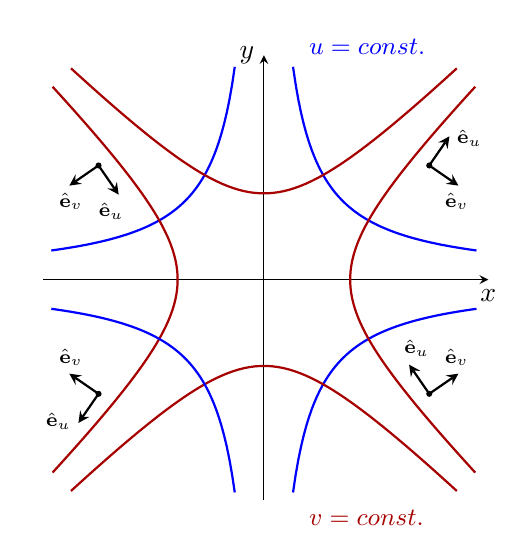
\begin{tikzpicture}[>=stealth]
\clip (-3,-3.2) rectangle (3,3.2);
\draw[->] (-2.8,0)--(2.85,0) node[below]{$x$};
\draw[->] (0,-2.8)--(0,2.85) node[left]{$y$};
\foreach \sg in {-1,1}{
 \draw[blue,thick,domain=0.37:2.7,samples=70] plot (\x,{\sg/\x});
 \draw[blue,thick,domain=-2.7:-0.37,samples=70] plot (\x,{\sg/\x});
 \draw[red!65!black,thick,domain=-2.45:2.45,samples=70]
 plot ({\sg*sqrt(1.2+\x*\x)},\x);
 \draw[red!65!black,thick,domain=-2.45:2.45,samples=70]
 plot (\x,{\sg*sqrt(1.2+\x*\x)});
}
\foreach \px/\py/\lux/\luy/\lvx/\lvy in {2.1/1.45/2.61/1.8/2.45/0.99,
 -2.1/1.45/-1.94/0.87/-2.45/0.99,-2.1/-1.45/-2.61/-1.8/-2.45/-0.99,
 2.1/-1.45/1.94/-0.87/2.45/-0.99}{
 \pgfmathsetmacro\fac{0.45/sqrt(\px*\px+\py*\py)}
 \fill (\px,\py) circle(1.1pt);
 \draw[->,black,thick] (\px,\py)--++({\fac*\py},{\fac*\px});
 \draw[->,black,thick] (\px,\py)--++({\fac*\px},{-\fac*\py});
 \node[font=\scriptsize] at (\lux,\luy){$\hat{\mathbf e}_u$};
 \node[font=\scriptsize] at (\lvx,\lvy){$\hat{\mathbf e}_v$};
}
\node[blue,font=\small,anchor=base west] at (0.45,2.86)
{$u=\text{const.}$};
\node[red!65!black,font=\small,anchor=base west] at (0.45,-3.12)
{$v=\text{const.}$};
\end{tikzpicture}
\end{center}
\textbf{(c)} For $\rho=\sqrt{x^2+y^2}>0$,
$\nabla u=(y,x,0)$ and $\nabla v=(2x,-2y,0)$.
They are orthogonal, since their dot product is $2xy-2xy=0$.
For orthogonal coordinates the gradient formula of Section 3.10,
$\nabla\psi=\sum_i\hat{\mathbf e}_i\,h_i^{-1}\,\partial\psi/\partial q_i$
with scale factors $h_i>0$, applied to $\psi=u$ and $\psi=v$ gives
$\nabla u=\hat{\mathbf e}_u/h_u$ and $\nabla v=\hat{\mathbf e}_v/h_v$.
Hence the increasing-coordinate unit vectors are $\nabla u/|\nabla u|$
and $\nabla v/|\nabla v|$, with $|\nabla u|=\sqrt{y^2+x^2}=\rho$ and
$|\nabla v|=2\rho$:
\[
\boxed{\hat{\mathbf e}_u=\frac{(y,x,0)}{\rho},\qquad
\hat{\mathbf e}_v=\frac{(x,-y,0)}{\rho}}.
\]
Their $(x,y)$ component signs in quadrants I, II, III, IV are
respectively $(+,+),(+,-),(-,-),(-,+)$ for $\hat{\mathbf e}_u$
and $(+,-),(-,-),(-,+),(+,+)$ for $\hat{\mathbf e}_v$.
\textbf{(d)} The cross product of the unit vectors is
\[
\hat{\mathbf e}_u\times\hat{\mathbf e}_v
=\rho^{-2}(y,x,0)\times(x,-y,0)
=\rho^{-2}\bigl(0,0,y(-y)-x\cdot x\bigr)
=-\hat{\mathbf e}_z,
\]
so the ordered system $(u,v,z)$ is left-handed.
\erratum{The chart is singular on the $z$-axis and is only local
unless a branch is chosen, because $(x,y)$ and $(-x,-y)$ have the
same $(u,v)$.}

One can also check handedness by the Jacobian. Differentiating the definitions gives
\[
\begin{pmatrix}du\\dv\end{pmatrix}
=\begin{pmatrix}y&x\\2x&-2y\end{pmatrix}
\begin{pmatrix}dx\\dy\end{pmatrix},\qquad
\det\frac{\partial(u,v)}{\partial(x,y)}=-2y^2-2x^2=-2(x^2+y^2).
\]
The rows of this matrix are $\nabla u$ and $\nabla v$, and
$\nabla u\times\nabla v=(0,0,-2y^2-2x^2)$ is this determinant times
$\hat{\mathbf e}_z$; so the negative determinant is the left-handedness
found in (d).
Inverting the $2\times2$ matrix with the rule
\[
\begin{pmatrix}\alpha&\beta\\\gamma&\delta\end{pmatrix}^{-1}
=\frac1{\alpha\delta-\beta\gamma}
\begin{pmatrix}\delta&-\beta\\-\gamma&\alpha\end{pmatrix}
\]
gives
\[
\frac{\partial(x,y)}{\partial(u,v)}
=\frac{1}{-2\rho^2}\begin{pmatrix}-2y&-x\\-2x&y\end{pmatrix}
=\begin{pmatrix}y/\rho^2&x/(2\rho^2)\\x/\rho^2&-y/(2\rho^2)\end{pmatrix},
\]
whose determinant is the reciprocal of the one above,
\[
\det\frac{\partial(x,y)}{\partial(u,v)}
=-\frac{y^2}{2\rho^4}-\frac{x^2}{2\rho^4}=-\frac1{2\rho^2}.
\]
The columns of the inverse matrix are the tangent vectors
$\partial\mathbf r/\partial u=(y,x,0)/\rho^2$ and
$\partial\mathbf r/\partial v=(x,-y,0)/(2\rho^2)$ of the coordinate
lines; as a check on (c), they point along $\hat{\mathbf e}_u$ and
$\hat{\mathbf e}_v$, with lengths $h_u=1/\rho$ and $h_v=1/(2\rho)$.
\erratum{The Instructor's Manual, p.~49, omits the factor $1/2$ in this
inverse determinant. Its earlier differential must likewise read
$dv=2x\,dx-2y\,dy$, with a minus sign, since
$\partial_y(x^2-y^2)=-2y$.}

\Needspace{5\baselineskip}
\par\bigskip
\noindent\textbf{3.10.2}\quad The elliptic cylindrical coordinate system
consists of three families of surfaces:
\[
\text{(1)}\ \frac{x^{2}}{a^{2}\cosh^{2}u}+\frac{y^{2}}{a^{2}\sinh^{2}u}=1;
\quad
\text{(2)}\ \frac{x^{2}}{a^{2}\cos^{2}v}-\frac{y^{2}}{a^{2}\sin^{2}v}=1;
\quad
\text{(3)}\ z=z.
\]
Sketch the coordinate surfaces $u=\text{constant}$ and $v=\text{constant}$ as
they intersect the first quadrant of the $xy$-plane. Show the unit vectors
$\hat{\mathbf{e}}_{u}$ and $\hat{\mathbf{e}}_{v}$. The range of $u$ is
$0\le u<\infty$. The range of $v$ is $0\le v\le2\pi$.
\erratum{Take $a>0$. Interpret the zero-denominator limiting surfaces by the parametrization below; the unit basis is undefined at the foci, where $\sinh^2u+\sin^2v=0$.}
\solution
Use the parametrization
\[
x=a\cosh u\cos v,\qquad y=a\sinh u\sin v,\qquad z=z,\quad a>0.
\]
Dividing its squared coordinates by $a^2\cosh^2u,a^2\sinh^2u$
and adding gives $1$; dividing by $a^2\cos^2v,a^2\sin^2v$
and subtracting also gives $1$. Thus it generates both stated families.
Constant $u>0$ gives ellipses with semi-axes $a\cosh u>a\sinh u$, whose
foci $(\pm c,0)$ have $c^2=a^2\cosh^2u-a^2\sinh^2u=a^2$; constant $v$
(not a multiple of $\pi/2$) gives hyperbolas with semi-axes
$a|\cos v|$ and $a|\sin v|$, whose foci $(\pm c,0)$ have
$c^2=a^2\cos^2v+a^2\sin^2v=a^2$. Both families are therefore confocal,
with foci $(\pm a,0)$. In the first quadrant use
$u>0$, $0<v<\pi/2$. The sketch shows the ellipses $u=0.45,0.8,1.15$
(blue), the hyperbolas $v=20^\circ,45^\circ,70^\circ$ (red), and the
unit vectors at the point $u=1$, $v=30^\circ$:
\begin{center}
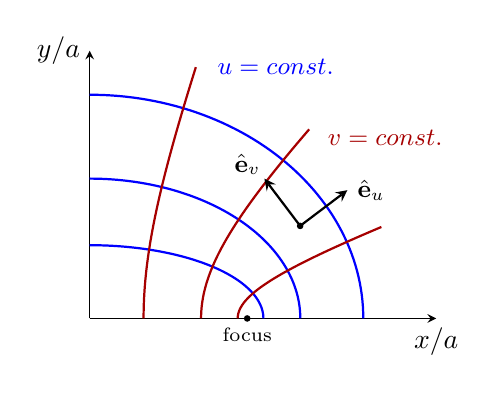
\begin{tikzpicture}[scale=2,>=stealth]
\draw[->] (0,0)--(2.2,0) node[below]{$x/a$};
\draw[->] (0,0)--(0,1.7) node[left]{$y/a$};
\foreach \u in {0.45,0.8,1.15}{
 \draw[blue,thick,domain=0:90,samples=60]
 plot ({(exp(\u)+exp(-\u))*cos(\x)/2},
       {(exp(\u)-exp(-\u))*sin(\x)/2});
}
\foreach \v in {20,45,70}{
 \draw[red!65!black,thick,domain=0:1.3,samples=60]
 plot ({(exp(\x)+exp(-\x))*cos(\v)/2},
       {(exp(\x)-exp(-\x))*sin(\v)/2});
}
\fill (1,0) circle(0.6pt) node[below,font=\scriptsize]{focus};
\coordinate (p) at (1.33635,0.58760);
\fill (p) circle(0.6pt);
\draw[->,thick] (p)--++(0.30,0.227)
 node[right,font=\small]{$\hat{\mathbf e}_u$};
\draw[->,thick] (p)--++(-0.227,0.30)
 node[above left,font=\small,inner sep=1pt]{$\hat{\mathbf e}_v$};
\node[blue,font=\small,anchor=west] at (0.75,1.6){$u=\text{const.}$};
\node[red!65!black,font=\small,anchor=west] at (1.45,1.15)
{$v=\text{const.}$};
\end{tikzpicture}
\end{center}
Differentiate the position:
\[
\frac{\partial\mathbf r}{\partial u}
=a(\sinh u\cos v,\ \cosh u\sin v,\ 0),\qquad
\frac{\partial\mathbf r}{\partial v}
=a(-\cosh u\sin v,\ \sinh u\cos v,\ 0).
\]
Both have squared length
\[
a^2(\sinh^2u\cos^2v+\cosh^2u\sin^2v)
=a^2[\sinh^2u(1-\sin^2v)+(1+\sinh^2u)\sin^2v]
=a^2(\sinh^2u+\sin^2v),
\]
and their dot product
$a^2(-\sinh u\cosh u\sin v\cos v+\cosh u\sinh u\sin v\cos v)$ is zero.
Normalizing,
\[
\boxed{\begin{aligned}
\hat{\mathbf e}_u&=
\frac{(\sinh u\cos v,\ \cosh u\sin v,\ 0)}
{\sqrt{\sinh^2u+\sin^2v}},\\
\hat{\mathbf e}_v&=
\frac{(-\cosh u\sin v,\ \sinh u\cos v,\ 0)}
{\sqrt{\sinh^2u+\sin^2v}}.
\end{aligned}}
\]
The common scale factor is $h_u=h_v=a\sqrt{\sinh^2u+\sin^2v}$.
The first vector points outward and northeast, the second along an
ellipse toward increasing $v$ (northwest) in this quadrant, since for
$u>0$, $0<v<\pi/2$ both $\sinh u\cos v$ and $\cosh u\sin v$ are
positive.
At limiting coordinate surfaces where a displayed denominator of the
implicit equations vanishes, use the parametrization and its limit:
in the $xy$-plane, $u=0$ gives the segment $|x|\le a$ of the $x$-axis,
$v=0$ and $v=\pi$ give the rays $x\ge a$ and $x\le-a$ of the $x$-axis,
and $v=\pi/2$ and $v=3\pi/2$ give the positive and negative $y$-axis.

\Needspace{5\baselineskip}
\par\bigskip
\noindent\textbf{3.10.3}\quad Develop arguments to show that dot and cross
products (not involving $\nabla$) in orthogonal curvilinear coordinates in
$\mathbb{R}^{3}$ proceed, as in Cartesian coordinates, \textbf{with no
involvement of scale factors}.
\erratum{Use physical components along orthonormal unit vectors; the usual cross-product signs require a right-handed ordering.}
\solution
At a fixed regular point, expand in the local orthonormal basis:
$\mathbf A=\sum_iA_i\hat{\mathbf e}_i$ and
$\mathbf B=\sum_jB_j\hat{\mathbf e}_j$. Both products are bilinear,
and the unit vectors of an orthogonal system satisfy
$\hat{\mathbf e}_i\cdot\hat{\mathbf e}_j=\delta_{ij}$, so
\[
\mathbf A\cdot\mathbf B
=\sum_{ij}A_iB_j\,\hat{\mathbf e}_i\cdot\hat{\mathbf e}_j
=\sum_{ij}A_iB_j\delta_{ij}=\sum_iA_iB_i.
\]
For a right-handed basis,
$\hat{\mathbf e}_1\times\hat{\mathbf e}_2=\hat{\mathbf e}_3$ and its
cyclic permutations hold, the reversed products change sign, and
$\hat{\mathbf e}_i\times\hat{\mathbf e}_i=0$; together,
$\hat{\mathbf e}_i\times\hat{\mathbf e}_j
=\sum_k\varepsilon_{ijk}\hat{\mathbf e}_k$, so
\[
\mathbf A\times\mathbf B
=\sum_{ij}A_iB_j\,\hat{\mathbf e}_i\times\hat{\mathbf e}_j
=\sum_{ijk}\varepsilon_{ijk}A_iB_j\hat{\mathbf e}_k.
\]
These are exactly the Cartesian component rules. Only the values of
the unit vectors at the one point enter, never their derivatives; the
scale factors appear only through $ds_i=h_i\,dq_i$ when $\nabla$
differentiates along the coordinate lines, which these products do not do.
\erratum{The usual cross-product sign assumes a right-handed unit
basis; a left-handed ordering, such as $(u,v,z)$ in Exercise 3.10.1, contributes
an overall minus sign.}
Also these formulas use physical components along unit vectors. Components
along the unnormalized coordinate tangents
$\partial\mathbf r/\partial q_i=h_i\hat{\mathbf e}_i$ would acquire
the corresponding scale factors.

\Needspace{5\baselineskip}
\par\bigskip
\noindent\textbf{3.10.4}\quad With $\hat{\mathbf{e}}_{1}$ a unit vector in the
direction of increasing $q_{1}$, show that
\begin{enumerate}
\item[(a)] $\displaystyle\nabla\cdot\hat{\mathbf{e}}_{1}
  =\frac{1}{h_{1}h_{2}h_{3}}\frac{\partial(h_{2}h_{3})}{\partial q_{1}}$
\item[(b)] $\displaystyle\nabla\times\hat{\mathbf{e}}_{1}
  =\frac{1}{h_{1}}\left[\hat{\mathbf{e}}_{2}\frac{1}{h_{3}}
  \frac{\partial h_{1}}{\partial q_{3}}
  -\hat{\mathbf{e}}_{3}\frac{1}{h_{2}}\frac{\partial h_{1}}{\partial q_{2}}
  \right]$.
\end{enumerate}
Note that even though $\hat{\mathbf{e}}_{1}$ is a unit vector, its divergence
and curl \textbf{do not necessarily vanish}.
\erratum{Use a regular, right-handed orthogonal coordinate chart with positive scale factors $h_i$.}
\solution
For physical components $V_i$ in an orthogonal system, the flux through
opposite $q_i$ faces gives
\[
\nabla\cdot\mathbf V=\frac1{h_1h_2h_3}
\sum_i\partial_{q_i}(h_jh_kV_i),\qquad\{i,j,k\}=\{1,2,3\}.
\]
For $\mathbf V=\hat{\mathbf e}_1$, $V_1=1,V_2=V_3=0$, so only the
$i=1$ term survives, $\partial_{q_1}(h_2h_3\cdot1)$, and
$\boxed{\nabla\cdot\hat{\mathbf e}_1=
(h_1h_2h_3)^{-1}\partial_{q_1}(h_2h_3)}$.
For the curl, the gradient formula
$\nabla\psi=\sum_j\hat{\mathbf e}_jh_j^{-1}\partial_{q_j}\psi$ with
$\psi=q_1$ gives $\nabla q_1=\hat{\mathbf e}_1/h_1$, i.e.\
$\hat{\mathbf e}_1=h_1\nabla q_1$. By the product rule
$\nabla\times(g\mathbf V)=\nabla g\times\mathbf V+g\nabla\times\mathbf V$
(Exercise 3.6.4) and $\nabla\times\nabla q_1=0$ (Exercise 3.6.10),
\[
\nabla\times\hat{\mathbf e}_1=\nabla h_1\times\nabla q_1
=\left(\sum_j\frac{\hat{\mathbf e}_j}{h_j}\partial_{q_j}h_1\right)
\times\frac{\hat{\mathbf e}_1}{h_1}.
\]
The $j=1$ term vanishes because $\hat{\mathbf e}_1\times\hat{\mathbf e}_1=0$.
In a right-handed basis
$\hat{\mathbf e}_2\times\hat{\mathbf e}_1=-\hat{\mathbf e}_3$ and
$\hat{\mathbf e}_3\times\hat{\mathbf e}_1=\hat{\mathbf e}_2$, so the
other two terms give
\[
\boxed{\nabla\times\hat{\mathbf e}_1=
\frac1{h_1}\left[
\frac{\hat{\mathbf e}_2}{h_3}\partial_{q_3}h_1
-\frac{\hat{\mathbf e}_3}{h_2}\partial_{q_2}h_1\right]}.
\]
For a left-handed ordering both cross products, and hence the result
of (b), change sign; this is why the note under the statement asks
for a right-handed chart.
The basis direction can vary even though its magnitude is fixed.

\Needspace{5\baselineskip}
\par\bigskip
\noindent\textbf{3.10.5}\quad Show that a set of orthogonal unit vectors
$\hat{\mathbf{e}}_{i}$ may be defined by
\[
\hat{\mathbf{e}}_{i}=\frac{1}{h_{i}}\frac{\partial\mathbf{r}}{\partial q_{i}}.
\]
In particular, show that $\hat{\mathbf{e}}_{i}\cdot\hat{\mathbf{e}}_{i}=1$
leads to an expression for $h_{i}$ in agreement with Eq.~(3.131).

The above equation for $\hat{\mathbf{e}}_{i}$ may be taken as a starting point
for deriving
\[
\frac{\partial\hat{\mathbf{e}}_{i}}{\partial q_{j}}
=\hat{\mathbf{e}}_{j}\frac{1}{h_{i}}\frac{\partial h_{j}}{\partial q_{i}},
\quad i\neq j
\]
and
\[
\frac{\partial\hat{\mathbf{e}}_{i}}{\partial q_{i}}
=-\sum_{j\neq i}\hat{\mathbf{e}}_{j}\frac{1}{h_{j}}
\frac{\partial h_{i}}{\partial q_{j}}.
\]
\erratum{Assume the coordinates form a regular orthogonal chart and $h_i>0$; arbitrary curvilinear coordinates need not be orthogonal.}
\solution
On a regular orthogonal chart, the tangent to increasing $q_i$ is
$\mathbf r_i=\partial_{q_i}\mathbf r$, and $\partial_i$ below means
$\partial/\partial q_i$. Since
$d\mathbf r=\sum_i\mathbf r_i\,dq_i$, the system is orthogonal exactly
when $\mathbf r_i\cdot\mathbf r_j=0$ for $i\ne j$ (no cross terms in
$ds^2=d\mathbf r\cdot d\mathbf r$), so the vectors
$\hat{\mathbf e}_i=\mathbf r_i/h_i$ are mutually orthogonal. Requiring
$\hat{\mathbf e}_i\cdot\hat{\mathbf e}_i=\mathbf r_i\cdot\mathbf r_i/h_i^2=1$
gives
\[
h_i^2=\mathbf r_i\cdot\mathbf r_i
=\Bigl(\frac{\partial x}{\partial q_i}\Bigr)^2
+\Bigl(\frac{\partial y}{\partial q_i}\Bigr)^2
+\Bigl(\frac{\partial z}{\partial q_i}\Bigr)^2,
\]
in agreement with Eq.~(3.131); then
$ds^2=\sum_ih_i^2dq_i^2$, so these $h_i$ are the scale factors.

To derive the basis derivatives, write
$\mathbf r_{ij}=\partial_j\mathbf r_i=\partial_i\partial_j\mathbf r$,
which is symmetric in $i,j$ because mixed partials commute.
Differentiating $\mathbf r_i=h_i\hat{\mathbf e}_i$ gives
$\mathbf r_{ij}=(\partial_jh_i)\hat{\mathbf e}_i+h_i\partial_j\hat{\mathbf e}_i$,
so $\mathbf r_{ij}=\mathbf r_{ji}$ reads
\[
(\partial_jh_i)\hat{\mathbf e}_i+h_i\partial_j\hat{\mathbf e}_i
=(\partial_ih_j)\hat{\mathbf e}_j+h_j\partial_i\hat{\mathbf e}_j.
\tag{*}
\]
Differentiating $\hat{\mathbf e}_i\cdot\hat{\mathbf e}_i=1$ with
respect to $q_j$ gives $\hat{\mathbf e}_i\cdot\partial_j\hat{\mathbf e}_i=0$.
For three distinct indices $i,j,k$, differentiate the orthogonality
relations $\mathbf r_i\cdot\mathbf r_k=0$, $\mathbf r_i\cdot\mathbf r_j=0$,
$\mathbf r_j\cdot\mathbf r_k=0$ with respect to $q_j$, $q_k$, $q_i$,
respectively; for example the first gives
$\mathbf r_{ij}\cdot\mathbf r_k+\mathbf r_i\cdot\mathbf r_{kj}=0$.
With the symmetry of $\mathbf r_{ij}$ the three results give, in turn,
\[
\mathbf r_k\cdot\mathbf r_{ij}
=-\mathbf r_i\cdot\mathbf r_{jk}
=\mathbf r_j\cdot\mathbf r_{ik}
=-\mathbf r_k\cdot\mathbf r_{ij},
\]
so $\mathbf r_k\cdot\mathbf r_{ij}=0$. Dotting the expansion of
$\mathbf r_{ij}$ with $\mathbf r_k=h_k\hat{\mathbf e}_k$ and using
$\hat{\mathbf e}_k\cdot\hat{\mathbf e}_i=0$ gives
$\mathbf r_k\cdot\mathbf r_{ij}=h_kh_i\,\hat{\mathbf e}_k\cdot\partial_j\hat{\mathbf e}_i$;
hence $\hat{\mathbf e}_k\cdot\partial_j\hat{\mathbf e}_i=0$.
Dotting (*) with $\hat{\mathbf e}_j$ for $i\ne j$, and using
$\hat{\mathbf e}_j\cdot\hat{\mathbf e}_i=0$ and
$\hat{\mathbf e}_j\cdot\partial_i\hat{\mathbf e}_j=0$, gives the only
remaining component:
$h_i\hat{\mathbf e}_j\cdot\partial_j\hat{\mathbf e}_i=\partial_i h_j$.
Therefore
\[
\boxed{\partial_j\hat{\mathbf e}_i
=\hat{\mathbf e}_j\,\frac{\partial_i h_j}{h_i}\quad(i\ne j)}.
\]
Finally, $\partial_i\hat{\mathbf e}_i$ has no $\hat{\mathbf e}_i$
component. For $j\ne i$ differentiate $\hat{\mathbf e}_i\cdot\hat{\mathbf e}_j=0$
with respect to $q_i$ and use the boxed formula with $i$ and $j$
interchanged, $\partial_i\hat{\mathbf e}_j=\hat{\mathbf e}_i(\partial_jh_i)/h_j$:
$\hat{\mathbf e}_j\cdot\partial_i\hat{\mathbf e}_i
=-\hat{\mathbf e}_i\cdot\partial_i\hat{\mathbf e}_j
=-(\partial_jh_i)/h_j$.
Expanding in the perpendicular basis gives
$\boxed{\partial_i\hat{\mathbf e}_i
=-\sum_{j\ne i}\hat{\mathbf e}_j(\partial_jh_i)/h_j}$.

\Needspace{5\baselineskip}
\par\bigskip
\noindent\textbf{3.10.6}\quad Resolve the circular cylindrical unit vectors
into their Cartesian components (see Fig.~3.23).
\par\nobreak\hfill\emph{ANS.}\enspace
$\begin{aligned}
\hat{\mathbf{e}}_{\rho}&=\hat{\mathbf{e}}_{x}\cos\varphi
+\hat{\mathbf{e}}_{y}\sin\varphi,\\
\hat{\mathbf{e}}_{\varphi}&=-\hat{\mathbf{e}}_{x}\sin\varphi
+\hat{\mathbf{e}}_{y}\cos\varphi,\\
\hat{\mathbf{e}}_{z}&=\hat{\mathbf{e}}_{z}.
\end{aligned}$
\solution
Start with $\mathbf r=(\rho\cos\varphi,\rho\sin\varphi,z)$.
Its coordinate derivatives are
\[
\partial_\rho\mathbf r=(\cos\varphi,\sin\varphi,0),\quad
\partial_\varphi\mathbf r=\rho(-\sin\varphi,\cos\varphi,0),\quad
\partial_z\mathbf r=(0,0,1).
\]
Their lengths are
$(\cos^2\varphi+\sin^2\varphi)^{1/2}=1$,
$\rho(\sin^2\varphi+\cos^2\varphi)^{1/2}=\rho$, and $1$, for $\rho>0$.
Dividing by these lengths gives
\[
\boxed{\hat{\mathbf e}_\rho=(\cos\varphi,\sin\varphi,0),\quad
\hat{\mathbf e}_\varphi=(-\sin\varphi,\cos\varphi,0),\quad
\hat{\mathbf e}_z=(0,0,1)}.
\]
Their dot products are $\delta_{ij}$ (for instance
$\hat{\mathbf e}_\rho\cdot\hat{\mathbf e}_\varphi
=-\cos\varphi\sin\varphi+\sin\varphi\cos\varphi=0$), and
$\hat{\mathbf e}_\rho\times\hat{\mathbf e}_\varphi
=(0,0,\cos^2\varphi+\sin^2\varphi)=\hat{\mathbf e}_z$, so the
ordering $(\rho,\varphi,z)$ is right-handed.

\Needspace{5\baselineskip}
\par\bigskip
\noindent\textbf{3.10.7}\quad Resolve the Cartesian unit vectors into their
circular cylindrical components (see Fig.~3.23).
\par\nobreak\hfill\emph{ANS.}\enspace
$\begin{aligned}
\hat{\mathbf{e}}_{x}&=\hat{\mathbf{e}}_{\rho}\cos\varphi
-\hat{\mathbf{e}}_{\varphi}\sin\varphi,\\
\hat{\mathbf{e}}_{y}&=\hat{\mathbf{e}}_{\rho}\sin\varphi
+\hat{\mathbf{e}}_{\varphi}\cos\varphi,\\
\hat{\mathbf{e}}_{z}&=\hat{\mathbf{e}}_{z}.
\end{aligned}$
\solution
Exercise 3.10.6 gives $\hat{\mathbf e}_\rho,\hat{\mathbf e}_\varphi,
\hat{\mathbf e}_z$ as the rows of an orthogonal matrix acting on
$(\hat{\mathbf e}_x,\hat{\mathbf e}_y,\hat{\mathbf e}_z)$; its inverse is
its transpose, whose first two rows are the first two columns
$(\cos\varphi,-\sin\varphi,0)$ and $(\sin\varphi,\cos\varphi,0)$ of
the original matrix. These rows give the coefficients of the
combinations, which check directly:
\[
\begin{aligned}
\cos\varphi\,\hat{\mathbf e}_\rho-\sin\varphi\,\hat{\mathbf e}_\varphi
&=(\cos^2\varphi+\sin^2\varphi,\ \cos\varphi\sin\varphi
-\sin\varphi\cos\varphi,\ 0)=\hat{\mathbf e}_x,\\
\sin\varphi\,\hat{\mathbf e}_\rho+\cos\varphi\,\hat{\mathbf e}_\varphi
&=(\sin\varphi\cos\varphi-\cos\varphi\sin\varphi,\
\sin^2\varphi+\cos^2\varphi,\ 0)=\hat{\mathbf e}_y.
\end{aligned}
\]
Together with unchanged $\hat{\mathbf e}_z$, these are the requested
inverse formulas.

\Needspace{5\baselineskip}
\par\bigskip
\noindent\textbf{3.10.8}\quad From the results of Exercise 3.10.6, show that
\[
\frac{\partial\hat{\mathbf{e}}_{\rho}}{\partial\varphi}
=\hat{\mathbf{e}}_{\varphi},\quad
\frac{\partial\hat{\mathbf{e}}_{\varphi}}{\partial\varphi}
=-\hat{\mathbf{e}}_{\rho}
\]
and that all other first derivatives of the circular cylindrical unit vectors
with respect to the circular cylindrical coordinates vanish.
\solution
Differentiating the Cartesian expressions gives
\[
\partial_\varphi\hat{\mathbf e}_\rho
=(-\sin\varphi,\cos\varphi,0)=\hat{\mathbf e}_\varphi,
\]
\[
\partial_\varphi\hat{\mathbf e}_\varphi
=(-\cos\varphi,-\sin\varphi,0)=-\hat{\mathbf e}_\rho.
\]
Neither depends on $\rho$ or $z$, so those derivatives vanish.
The vector $\hat{\mathbf e}_z=(0,0,1)$ is constant, so all three
of its coordinate derivatives vanish.

\Needspace{5\baselineskip}
\par\bigskip
\noindent\textbf{3.10.9}\quad Compare $\nabla\cdot\mathbf{V}$ as given for
cylindrical coordinates in Eq.~(3.148) with the result of its computation by
applying to $\mathbf{V}$ the operator
\[
\nabla=\hat{\mathbf{e}}_{\rho}\frac{\partial}{\partial\rho}
+\hat{\mathbf{e}}_{\varphi}\frac{1}{\rho}\frac{\partial}{\partial\varphi}
+\hat{\mathbf{e}}_{z}\frac{\partial}{\partial z}
\]
Note that $\nabla$ acts both on the unit vectors and on the components of
$\mathbf{V}$.
\solution
Write $\mathbf V=V_\rho\hat{\mathbf e}_\rho+
V_\varphi\hat{\mathbf e}_\varphi+V_z\hat{\mathbf e}_z$.
The basis has no $\rho$ or $z$ dependence, giving
$\hat{\mathbf e}_\rho\cdot\partial_\rho\mathbf V=\partial_\rho V_\rho$
and $\hat{\mathbf e}_z\cdot\partial_z\mathbf V=\partial_zV_z$.
For the azimuthal derivative, differentiate coefficients and basis,
using $\partial_\varphi\hat{\mathbf e}_\rho=\hat{\mathbf e}_\varphi$ and
$\partial_\varphi\hat{\mathbf e}_\varphi=-\hat{\mathbf e}_\rho$
(Exercise 3.10.8):
\[
\partial_\varphi\mathbf V
=(\partial_\varphi V_\rho-V_\varphi)\hat{\mathbf e}_\rho
+(\partial_\varphi V_\varphi+V_\rho)\hat{\mathbf e}_\varphi
+(\partial_\varphi V_z)\hat{\mathbf e}_z.
\]
The operator gives
$\nabla\cdot\mathbf V=\hat{\mathbf e}_\rho\cdot\partial_\rho\mathbf V
+\rho^{-1}\hat{\mathbf e}_\varphi\cdot\partial_\varphi\mathbf V
+\hat{\mathbf e}_z\cdot\partial_z\mathbf V$, and with
$\hat{\mathbf e}_\varphi\cdot\partial_\varphi\mathbf V
=\partial_\varphi V_\varphi+V_\rho$ from the last display, the three
dot products yield
\[
\boxed{\nabla\cdot\mathbf V
=\partial_\rho V_\rho+\frac{V_\rho}{\rho}
+\frac1\rho\partial_\varphi V_\varphi+\partial_zV_z
=\frac1\rho\partial_\rho(\rho V_\rho)
+\frac1\rho\partial_\varphi V_\varphi+\partial_zV_z},
\]
where $\rho^{-1}\partial_\rho(\rho V_\rho)=\partial_\rho V_\rho+V_\rho/\rho$.
This agrees with Eq.~(3.148).
The $V_\rho/\rho$ term is exactly the contribution of the varying basis.

\erratum{The Instructor's Manual, p.~51, calls the exercise's operator incorrect. The textbook explicitly says that it acts on the unit vectors as well as the components, so the operator as stated is correct: the basis derivative supplies exactly the $V_\rho/\rho$ term computed above.}

\Needspace{5\baselineskip}
\par\bigskip
\noindent\textbf{3.10.10}\quad
\begin{enumerate}
\item[(a)] Show that
  $\mathbf{r}=\hat{\mathbf{e}}_{\rho}\rho+\hat{\mathbf{e}}_{z}z$.
\item[(b)] Working entirely in circular cylindrical coordinates, show that
  \[
  \nabla\cdot\mathbf{r}=3\quad\text{and}\quad\nabla\times\mathbf{r}=0.
  \]
\end{enumerate}
\solution
\textbf{(a)} Since $x=\rho\cos\varphi,y=\rho\sin\varphi$,
$x\hat{\mathbf e}_x+y\hat{\mathbf e}_y
=\rho(\cos\varphi\,\hat{\mathbf e}_x+\sin\varphi\,\hat{\mathbf e}_y)
=\rho\hat{\mathbf e}_\rho$ by Exercise 3.10.6,
so $\mathbf r=\rho\hat{\mathbf e}_\rho+z\hat{\mathbf e}_z$.

\textbf{(b)} The physical cylindrical components of $\mathbf r$ are
$(V_\rho,V_\varphi,V_z)=(\rho,0,z)$.
Therefore Eq.~(3.148) gives
\[
\nabla\cdot\mathbf r=\frac1\rho\partial_\rho(\rho^2)
+\frac1\rho\partial_\varphi0+\partial_zz=2+0+1=3.
\]
For the curl, expanding the determinant form of the curl with
$h_\rho=1$, $h_\varphi=\rho$, $h_z=1$ gives the components
\[
(\nabla\times\mathbf V)_\rho=\frac1\rho\partial_\varphi V_z-\partial_zV_\varphi,\quad
(\nabla\times\mathbf V)_\varphi=\partial_zV_\rho-\partial_\rho V_z,\quad
(\nabla\times\mathbf V)_z=\frac1\rho[\partial_\rho(\rho V_\varphi)-\partial_\varphi V_\rho].
\]
For $\mathbf V=\mathbf r$,
\[
(\nabla\times\mathbf r)_\rho=\rho^{-1}\partial_\varphi z-\partial_z0=0,
\quad
(\nabla\times\mathbf r)_\varphi=\partial_z\rho-\partial_\rho z=0,
\]
and
$(\nabla\times\mathbf r)_z=\rho^{-1}[\partial_\rho(\rho\,0)-\partial_\varphi\rho]=0$.
Thus $\boxed{\nabla\times\mathbf r=0}$.

\Needspace{5\baselineskip}
\par\bigskip
\noindent\textbf{3.10.11}\quad
\begin{enumerate}
\item[(a)] Show that the parity operation (reflection through the origin) on a
  point $(\rho,\varphi,z)$ relative to fixed $x$-, $y$-, $z$-axes consists of
  the transformation
  \[
  \rho\to\rho,\quad\varphi\to\varphi\pm\pi,\quad z\to-z.
  \]
\item[(b)] Show that $\hat{\mathbf{e}}_{\rho}$ and $\hat{\mathbf{e}}_{\varphi}$
  have odd parity (reversal of direction) and that $\hat{\mathbf{e}}_{z}$ has
  even parity.
\end{enumerate}
\emph{Note.}~The Cartesian unit vectors $\hat{\mathbf{e}}_{x}$,
$\hat{\mathbf{e}}_{y}$, and $\hat{\mathbf{e}}_{z}$ remain constant.
\solution
\textbf{(a)} Under $(x,y,z)\mapsto(-x,-y,-z)$,
$\rho=\sqrt{x^2+y^2}$ is unchanged. Both $\cos\varphi=x/\rho$
and $\sin\varphi=y/\rho$ change sign. Since
$\cos(\varphi\pm\pi)=-\cos\varphi$, $\sin(\varphi\pm\pi)=-\sin\varphi$,
and the pair $(\cos\varphi,\sin\varphi)$ fixes the angle modulo $2\pi$,
$\varphi\mapsto\varphi\pm\pi$ (the two signs give the same point);
and $z\mapsto-z$.

\textbf{(b)} Substituting this angle into the unit-vector functions of
Exercise 3.10.6 gives
\[
\begin{aligned}
\hat{\mathbf e}_\rho(\varphi+\pi)&=(-\cos\varphi,-\sin\varphi,0)
=-\hat{\mathbf e}_\rho(\varphi),\\
\hat{\mathbf e}_\varphi(\varphi+\pi)&=(\sin\varphi,-\cos\varphi,0)
=-\hat{\mathbf e}_\varphi(\varphi),\\
\hat{\mathbf e}_z(\varphi+\pi)&=(0,0,1)=\hat{\mathbf e}_z.
\end{aligned}
\]
This is evaluation of the curvilinear basis at the reflected point
relative to fixed Cartesian unit vectors, as specified in the note.

\Needspace{5\baselineskip}
\par\bigskip
\noindent\textbf{3.10.12}\quad A rigid body is rotating about a fixed axis
with a constant angular velocity $\boldsymbol{\omega}$. Take
$\boldsymbol{\omega}$ to lie along the $z$-axis. Express the position vector
$\mathbf{r}$ in circular cylindrical coordinates and using circular
cylindrical coordinates,
\begin{enumerate}
\item[(a)] calculate $\mathbf{v}=\boldsymbol{\omega}\times\mathbf{r}$,
\item[(b)] calculate $\nabla\times\mathbf{v}$.
\end{enumerate}
\par\nobreak\hfill\emph{ANS.}\enspace
(a)\enspace$\mathbf{v}=\hat{\mathbf{e}}_{\varphi}\omega\rho$\quad
(b)\enspace$\nabla\times\mathbf{v}=2\boldsymbol{\omega}$.
\solution
\textbf{(a)} With $\boldsymbol\omega=\omega\hat{\mathbf e}_z$ and
$\mathbf r=\rho\hat{\mathbf e}_\rho+z\hat{\mathbf e}_z$
(Exercise 3.10.10), and the right-handed products
$\hat{\mathbf e}_z\times\hat{\mathbf e}_\rho=\hat{\mathbf e}_\varphi$,
$\hat{\mathbf e}_z\times\hat{\mathbf e}_z=0$,
\[
\mathbf v=\omega\hat{\mathbf e}_z\times
(\rho\hat{\mathbf e}_\rho+z\hat{\mathbf e}_z)
=\omega\rho\,\hat{\mathbf e}_z\times\hat{\mathbf e}_\rho
=\boxed{\omega\rho\hat{\mathbf e}_\varphi}.
\]
\textbf{(b)} Its components are $(v_\rho,v_\varphi,v_z)=(0,\omega\rho,0)$
and are independent of $z,\varphi$. Hence, with the cylindrical curl
components of Exercise 3.10.10,
$(\nabla\times\mathbf v)_\rho=\rho^{-1}\partial_\varphi0-\partial_z(\omega\rho)=0$
and $(\nabla\times\mathbf v)_\varphi=\partial_z0-\partial_\rho0=0$, while
\[
(\nabla\times\mathbf v)_z
=\frac1\rho[\partial_\rho(\rho\,\omega\rho)-\partial_\varphi0]
=\frac{2\omega\rho}{\rho}=2\omega.
\]
Thus $\boxed{\nabla\times\mathbf v=2\omega\hat{\mathbf e}_z=2\boldsymbol\omega}$.

\Needspace{5\baselineskip}
\par\bigskip
\noindent\textbf{3.10.13}\quad Find the circular cylindrical components of the
velocity and acceleration of a moving particle,
\[
\begin{aligned}
v_{\rho}&=\dot{\rho},&a_{\rho}&=\ddot{\rho}-\rho\dot{\varphi}^{2},\\
v_{\varphi}&=\rho\dot{\varphi},&a_{\varphi}&=\rho\ddot{\varphi}
+2\dot{\rho}\dot{\varphi},\\
v_{z}&=\dot{z},&a_{z}&=\ddot{z}.
\end{aligned}
\]
\emph{Hint.}\quad
$\begin{aligned}[t]
\mathbf{r}(t)&=\hat{\mathbf{e}}_{\rho}(t)\rho(t)+\hat{\mathbf{e}}_{z}z(t)\\
&=[\hat{\mathbf{e}}_{x}\cos\varphi(t)+\hat{\mathbf{e}}_{y}\sin\varphi(t)]
\rho(t)+\hat{\mathbf{e}}_{z}z(t).
\end{aligned}$

\emph{Note.}~$\dot{\rho}=d\rho/dt$, $\ddot{\rho}=d^{2}\rho/dt^{2}$, and so on.
\solution
Along the trajectory the unit vectors depend on $t$ only through
$\varphi(t)$, so by the chain rule and Exercise 3.10.8 the basis
derivatives are
$\dot{\hat{\mathbf e}}_\rho=\dot\varphi\,\partial_\varphi\hat{\mathbf e}_\rho
=\dot\varphi\hat{\mathbf e}_\varphi$,
$\dot{\hat{\mathbf e}}_\varphi=\dot\varphi\,\partial_\varphi\hat{\mathbf e}_\varphi
=-\dot\varphi\hat{\mathbf e}_\rho$,
and $\dot{\hat{\mathbf e}}_z=0$.
(Differentiating the hint's Cartesian form directly gives the same:
$\frac d{dt}(\cos\varphi,\sin\varphi,0)=\dot\varphi(-\sin\varphi,\cos\varphi,0)$.)
Differentiate $\mathbf r=\rho\hat{\mathbf e}_\rho+z\hat{\mathbf e}_z$
by the product rule:
\[
\mathbf v=\dot\rho\hat{\mathbf e}_\rho+
\rho\dot\varphi\hat{\mathbf e}_\varphi+\dot z\hat{\mathbf e}_z.
\]
Differentiate each term once more, again with
$\dot{\hat{\mathbf e}}_\rho=\dot\varphi\hat{\mathbf e}_\varphi$ and
$\dot{\hat{\mathbf e}}_\varphi=-\dot\varphi\hat{\mathbf e}_\rho$:
\[
\begin{aligned}
\mathbf a={}&\underbrace{\ddot\rho\hat{\mathbf e}_\rho+
\dot\rho\dot\varphi\hat{\mathbf e}_\varphi}_{d(\dot\rho\hat{\mathbf e}_\rho)/dt}
+\underbrace{(\dot\rho\dot\varphi+\rho\ddot\varphi)\hat{\mathbf e}_\varphi
-\rho\dot\varphi^2\hat{\mathbf e}_\rho}_{d(\rho\dot\varphi\hat{\mathbf e}_\varphi)/dt}
+\ddot z\hat{\mathbf e}_z.
\end{aligned}
\]
Collecting coefficients gives
\[
\boxed{\begin{aligned}
v_\rho&=\dot\rho,&v_\varphi&=\rho\dot\varphi,&v_z&=\dot z,\\
a_\rho&=\ddot\rho-\rho\dot\varphi^2,&
a_\varphi&=\rho\ddot\varphi+2\dot\rho\dot\varphi,&a_z&=\ddot z.
\end{aligned}}
\]

\Needspace{5\baselineskip}
\par\bigskip
\noindent\textbf{3.10.14}\quad In right circular cylindrical coordinates, a
particular vector function is given by
\[
\mathbf{V}(\rho,\varphi)=\hat{\mathbf{e}}_{\rho}V_{\rho}(\rho,\varphi)
+\hat{\mathbf{e}}_{\varphi}V_{\varphi}(\rho,\varphi).
\]
Show that $\nabla\times\mathbf{V}$ has only a $z$-component. Note that this
result will hold for any vector confined to a surface $q_{3}=\text{constant}$
as long as the products $h_{1}V_{1}$ and $h_{2}V_{2}$ are each independent of
$q_{3}$.
\solution
Use the cylindrical curl components of Exercise 3.10.10 with $V_z=0$
and the absence of $z$ dependence:
\[
(\nabla\times\mathbf V)_\rho=\rho^{-1}\partial_\varphi V_z-\partial_zV_\varphi=0,
\qquad
(\nabla\times\mathbf V)_\varphi=\partial_zV_\rho-\partial_\rho V_z=0.
\]
The remaining component need not vanish:
\[
\boxed{\nabla\times\mathbf V=
\frac{\hat{\mathbf e}_z}{\rho}
[\partial_\rho(\rho V_\varphi)-\partial_\varphi V_\rho]}.
\]
More generally, expanding the determinant form of the curl in
orthogonal coordinates gives the first two components
\[
(\nabla\times\mathbf V)_1=\frac{\partial_2(h_3V_3)-\partial_3(h_2V_2)}{h_2h_3},
\qquad
(\nabla\times\mathbf V)_2=\frac{\partial_3(h_1V_1)-\partial_1(h_3V_3)}{h_3h_1},
\]
with $\partial_i=\partial/\partial q_i$. For a vector confined to the
surfaces $q_3=\text{constant}$, $V_3=0$, and these reduce to
\[
-(h_2h_3)^{-1}\partial_3(h_2V_2),\qquad
(h_3h_1)^{-1}\partial_3(h_1V_1).
\]
Both vanish when $h_1V_1$ and $h_2V_2$ are independent of $q_3$, as
stated in the problem, leaving only component 3. (Cylindrical
coordinates with $q_3=z$, $h_1V_1=V_\rho$, $h_2V_2=\rho V_\varphi$ are
the case above.)

\erratum{For this $V_z=0$ field, the transverse curl components are $-\partial_zV_\varphi$ and $\partial_zV_\rho$. The Instructor's Manual, p.~52, gives the first with the wrong sign and the second with an extra factor $1/\rho$. Both are zero here because the components are independent of $z$, so the conclusion survives those errors.}

\Needspace{5\baselineskip}
\par\bigskip
\noindent\textbf{3.10.15}\quad A conducting wire along the $z$-axis carries a
current $I$. The resulting magnetic vector potential is given by
\[
\mathbf{A}=\hat{\mathbf{e}}_{z}\frac{\mu I}{2\pi}\ln\frac{1}{\rho}.
\]
Show that the magnetic induction $\mathbf{B}$ is given by
\[
\mathbf{B}=\hat{\mathbf{e}}_{\varphi}\frac{\mu I}{2\pi\rho}.
\]
\solution
Let $K=\mu I/(2\pi)$, so $A_z=K\ln(1/\rho)=-K\ln\rho$, $A_\rho=A_\varphi=0$.
With the cylindrical curl components of Exercise 3.10.10,
$B_\rho=\rho^{-1}\partial_\varphi A_z-\partial_zA_\varphi=0$ because
$A_z$ does not depend on $\varphi$, and
$B_z=\rho^{-1}[\partial_\rho(\rho A_\varphi)-\partial_\varphi A_\rho]=0$.
The remaining one is
\[
B_\varphi=\partial_zA_\rho-\partial_\rho A_z
=0-(-K/\rho)=K/\rho.
\]
Thus $\boxed{\mathbf B=\mu I\,\hat{\mathbf e}_\varphi/(2\pi\rho)}$,
valid for $\rho>0$ outside the ideal wire.
Replacing $\ln(1/\rho)$ by $\ln(\rho_0/\rho)$ makes the logarithm
dimensionless and adds only a constant to $A_z$, leaving $\mathbf B$ unchanged.

\Needspace{5\baselineskip}
\par\bigskip
\noindent\textbf{3.10.16}\quad A force is described by
\[
\mathbf{F}=-\hat{\mathbf{e}}_{x}\frac{y}{x^{2}+y^{2}}
+\hat{\mathbf{e}}_{y}\frac{x}{x^{2}+y^{2}}.
\]
\begin{enumerate}
\item[(a)] Express $\mathbf{F}$ in circular cylindrical coordinates.

  Operating entirely in circular cylindrical coordinates for (b) and (c),
\item[(b)] Calculate the curl of $\mathbf{F}$ and
\item[(c)] Calculate the work done by $\mathbf{F}$ in encircling the unit
  circle once counterclockwise.
\item[(d)] How do you reconcile the results of (b) and (c)?
\end{enumerate}
\solution
\textbf{(a)} Substitute $x=\rho\cos\varphi,y=\rho\sin\varphi$, so
$x^2+y^2=\rho^2$:
\[
\mathbf F=\frac{(-\rho\sin\varphi,\rho\cos\varphi,0)}{\rho^2}
=\frac1\rho(-\sin\varphi,\cos\varphi,0)
=\boxed{\hat{\mathbf e}_\varphi/\rho}.
\]
\textbf{(b)} For $\rho>0$, $F_\rho=F_z=0$ and $F_\varphi=1/\rho$ depends
on $\rho$ only. With the cylindrical curl components of
Exercise 3.10.10, the transverse components
$\rho^{-1}\partial_\varphi F_z-\partial_zF_\varphi$ and
$\partial_zF_\rho-\partial_\rho F_z$ vanish,
and $(\nabla\times\mathbf F)_z=\rho^{-1}[\partial_\rho(\rho\cdot\rho^{-1})
-\partial_\varphi F_\rho]=\rho^{-1}\partial_\rho1=0$.
So $\boxed{\nabla\times\mathbf F=0}$ for $\rho>0$.
\textbf{(c)} In cylindrical coordinates
$d\mathbf r=\hat{\mathbf e}_\rho d\rho+\hat{\mathbf e}_\varphi\rho\,d\varphi
+\hat{\mathbf e}_z dz$; on the unit circle ($\rho=1$, $z=0$)
$d\mathbf r=\hat{\mathbf e}_\varphi d\varphi$ and
$\mathbf F\cdot d\mathbf r=d\varphi$, so
$\boxed{W=\oint\mathbf F\cdot d\mathbf r=\int_0^{2\pi}d\varphi=2\pi}$.
\textbf{(d)} The field is undefined on the axis. A disk spanning
the circle crosses that singularity, so Stokes' theorem cannot
use the ordinary zero curl over that disk. On an annulus excluding
the axis, the outer counterclockwise circulation $2\pi$ and the
inner clockwise circulation $-2\pi$ cancel, in full agreement with
zero curl. (The calculation in (c) gives $2\pi$ on a circle of any
radius $a$, since $\mathbf F\cdot d\mathbf r=a^{-1}\,a\,d\varphi$.)
Locally $\mathbf F=\nabla\varphi$, since
$\nabla\varphi=\hat{\mathbf e}_\varphi\rho^{-1}\partial_\varphi\varphi
=\hat{\mathbf e}_\varphi/\rho$, but $\varphi$ is not
a global single-valued potential around the axis: it increases by
$2\pi$ once around, which is the circulation found in (c).

\Needspace{5\baselineskip}
\par\bigskip
\noindent\textbf{3.10.17}\quad A calculation of the magnetohydrodynamic pinch
effect involves the evaluation of $(\mathbf{B}\cdot\nabla)\mathbf{B}$. If the
magnetic induction $\mathbf{B}$ is taken to be
$\mathbf{B}=\hat{\mathbf{e}}_{\varphi}B_{\varphi}(\rho)$, show that
\[
(\mathbf{B}\cdot\nabla)\mathbf{B}
=-\hat{\mathbf{e}}_{\rho}B_{\varphi}^{2}/\rho.
\]
\solution
For $\mathbf B=B_\varphi(\rho)\hat{\mathbf e}_\varphi$, dotting into
$\nabla=\hat{\mathbf e}_\rho\partial_\rho
+\hat{\mathbf e}_\varphi\rho^{-1}\partial_\varphi+\hat{\mathbf e}_z\partial_z$
keeps only the middle term, so
the directional derivative operator is
$\mathbf B\cdot\nabla=(B_\varphi/\rho)\partial_\varphi$.
It must differentiate the basis as well as the scalar component:
\[
(\mathbf B\cdot\nabla)\mathbf B
=\frac{B_\varphi}{\rho}
\left[(\partial_\varphi B_\varphi)\hat{\mathbf e}_\varphi+
B_\varphi\partial_\varphi\hat{\mathbf e}_\varphi\right]
=\boxed{-\frac{B_\varphi^2}{\rho}\hat{\mathbf e}_\rho}.
\]
Here $\partial_\varphi B_\varphi=0$ and
$\partial_\varphi\hat{\mathbf e}_\varphi=-\hat{\mathbf e}_\rho$
(Exercise 3.10.8).

\Needspace{5\baselineskip}
\par\bigskip
\noindent\textbf{3.10.18}\quad Express the spherical polar unit vectors in
terms of Cartesian unit vectors.
\par\nobreak\hfill\emph{ANS.}\enspace
$\begin{aligned}
\hat{\mathbf{e}}_{r}&=\hat{\mathbf{e}}_{x}\sin\theta\cos\varphi
+\hat{\mathbf{e}}_{y}\sin\theta\sin\varphi+\hat{\mathbf{e}}_{z}\cos\theta,\\
\hat{\mathbf{e}}_{\theta}&=\hat{\mathbf{e}}_{x}\cos\theta\cos\varphi
+\hat{\mathbf{e}}_{y}\cos\theta\sin\varphi-\hat{\mathbf{e}}_{z}\sin\theta,\\
\hat{\mathbf{e}}_{\varphi}&=-\hat{\mathbf{e}}_{x}\sin\varphi
+\hat{\mathbf{e}}_{y}\cos\varphi.
\end{aligned}$
\solution
The position map is
$\mathbf r=r(\sin\theta\cos\varphi,\sin\theta\sin\varphi,\cos\theta)$.
Its $r,\theta,\varphi$ derivatives are
\[
\begin{aligned}
\partial_r\mathbf r&=(\sin\theta\cos\varphi,\sin\theta\sin\varphi,\cos\theta),\\
\partial_\theta\mathbf r&=r(\cos\theta\cos\varphi,\cos\theta\sin\varphi,-\sin\theta),\\
\partial_\varphi\mathbf r&=r\sin\theta(-\sin\varphi,\cos\varphi,0),
\end{aligned}
\]
with lengths $1,r,r\sin\theta$ on a regular patch $r>0$, $0<\theta<\pi$
(for the first two, the squared components sum to
$\sin^2\theta+\cos^2\theta=1$ after $\cos^2\varphi+\sin^2\varphi=1$).
Normalize each derivative to obtain
\[
\boxed{\begin{aligned}
\hat{\mathbf e}_r&=(\sin\theta\cos\varphi,\sin\theta\sin\varphi,\cos\theta),\\
\hat{\mathbf e}_\theta&=(\cos\theta\cos\varphi,\cos\theta\sin\varphi,-\sin\theta),\\
\hat{\mathbf e}_\varphi&=(-\sin\varphi,\cos\varphi,0).
\end{aligned}}
\]
Their norms are one, their pairwise dot products vanish (for instance
$\hat{\mathbf e}_r\cdot\hat{\mathbf e}_\theta
=\sin\theta\cos\theta(\cos^2\varphi+\sin^2\varphi)-\cos\theta\sin\theta=0$),
and
\[
\hat{\mathbf e}_r\times\hat{\mathbf e}_\theta
=\bigl(-\sin\varphi(\sin^2\theta+\cos^2\theta),\
\cos\varphi(\cos^2\theta+\sin^2\theta),\ 0\bigr)
=\hat{\mathbf e}_\varphi,
\]
so $(r,\theta,\varphi)$ is right-handed.
At the polar axis, the angular basis requires a choice of azimuthal
limit and is not a unique coordinate basis.

\Needspace{5\baselineskip}
\par\bigskip
\noindent\textbf{3.10.19}\quad Resolve the Cartesian unit vectors into their
spherical polar components:
\[
\begin{aligned}
\hat{\mathbf{e}}_{x}&=\hat{\mathbf{e}}_{r}\sin\theta\cos\varphi
+\hat{\mathbf{e}}_{\theta}\cos\theta\cos\varphi
-\hat{\mathbf{e}}_{\varphi}\sin\varphi,\\
\hat{\mathbf{e}}_{y}&=\hat{\mathbf{e}}_{r}\sin\theta\sin\varphi
+\hat{\mathbf{e}}_{\theta}\cos\theta\sin\varphi
+\hat{\mathbf{e}}_{\varphi}\cos\varphi,\\
\hat{\mathbf{e}}_{z}&=\hat{\mathbf{e}}_{r}\cos\theta
-\hat{\mathbf{e}}_{\theta}\sin\theta.
\end{aligned}
\]
\solution
Any vector is the sum of its projections on an orthonormal basis.
For example,
$\hat{\mathbf e}_x=\sum_{j=r,\theta,\varphi}
(\hat{\mathbf e}_x\cdot\hat{\mathbf e}_j)\hat{\mathbf e}_j$.
The projection coefficients
$\hat{\mathbf e}_x\cdot\hat{\mathbf e}_r=\sin\theta\cos\varphi$,
$\hat{\mathbf e}_x\cdot\hat{\mathbf e}_\theta=\cos\theta\cos\varphi$,
$\hat{\mathbf e}_x\cdot\hat{\mathbf e}_\varphi=-\sin\varphi$
are precisely the $x$ components of the vectors in Exercise 3.10.18.
Repeating with their $y$ and $z$ components gives
\[
\boxed{\begin{aligned}
\hat{\mathbf e}_x&=\sin\theta\cos\varphi\,\hat{\mathbf e}_r
+\cos\theta\cos\varphi\,\hat{\mathbf e}_\theta-\sin\varphi\,\hat{\mathbf e}_\varphi,\\
\hat{\mathbf e}_y&=\sin\theta\sin\varphi\,\hat{\mathbf e}_r
+\cos\theta\sin\varphi\,\hat{\mathbf e}_\theta+\cos\varphi\,\hat{\mathbf e}_\varphi,\\
\hat{\mathbf e}_z&=\cos\theta\,\hat{\mathbf e}_r-\sin\theta\,\hat{\mathbf e}_\theta.
\end{aligned}}
\]
Thus the inverse change-of-basis matrix is the transpose of the matrix
whose rows are the vectors of Exercise 3.10.18 (the matrix $T$ of
Exercise 3.10.20).

\Needspace{5\baselineskip}
\par\bigskip
\noindent\textbf{3.10.20}\quad
\begin{enumerate}
\item[(a)] Explain why it is not possible to relate a column vector
  $\mathbf{r}$ (with components $x,y,z$) to another column vector
  $\mathbf{r}'$ (with components $r,\theta,\varphi$), via a matrix equation of
  the form $\mathbf{r}'=\mathsf{B}\mathbf{r}$ \erratum{with one constant matrix $\mathsf B$ valid at all positions}.
\item[(b)] One can write a matrix equation relating the Cartesian components
  of a vector to its components in spherical polar coordinates. Find the
  transformation matrix and determine whether it is orthogonal.
\end{enumerate}
\solution
\textbf{(a)} \erratum{The qualification ``one constant matrix'' is
needed: at any one point $\mathbf r\ne0$ the position-dependent matrix
$\mathsf B=\mathbf r'\mathbf r^T/r^2$ does give
$\mathsf B\mathbf r=\mathbf r'(\mathbf r^T\mathbf r)/r^2=\mathbf r'$.}
Write $\mathbf x=(x,y,z)^T$ for the column $\mathbf r$, to keep it
apart from the radius $r$. The radius $r=\sqrt{x^2+y^2+z^2}$ is not
a linear function: $r(-\mathbf x)=r(\mathbf x)$, whereas the first
component of a constant matrix map is linear,
$(\mathsf B(-\mathbf x))_1=-(\mathsf B\mathbf x)_1$.
If $(\mathsf B\mathbf x)_1=r(\mathbf x)$ held for all $\mathbf x$, then
$r(\mathbf x)=r(-\mathbf x)=(\mathsf B(-\mathbf x))_1
=-(\mathsf B\mathbf x)_1=-r(\mathbf x)$, so $r(\mathbf x)=0$, which is
false for $\mathbf x\ne0$.
The angular coordinates are nonlinear as well; for example
$\theta(2\mathbf x)=\theta(\mathbf x)$, while a linear function doubles.

\textbf{(b)} Physical components of a vector at a fixed point are its
projections on the unit vectors, $V_r=\hat{\mathbf e}_r\cdot\mathbf V
=\sum_a(\hat{\mathbf e}_r)_aV_a$ and similarly for $V_\theta,V_\varphi$,
with the Cartesian components $(\hat{\mathbf e}_r)_a$ etc.\ of
Exercise 3.10.18. Hence they obey
\[
\boxed{\begin{pmatrix}V_r\\V_\theta\\V_\varphi\end{pmatrix}
=T\begin{pmatrix}V_x\\V_y\\V_z\end{pmatrix},\quad
T=\begin{pmatrix}
\sin\theta\cos\varphi&\sin\theta\sin\varphi&\cos\theta\\
\cos\theta\cos\varphi&\cos\theta\sin\varphi&-\sin\theta\\
-\sin\varphi&\cos\varphi&0
\end{pmatrix}}.
\]
The rows are the three unit vectors from Exercise 3.10.18, so the
entries of $TT^T$ are their inner products,
$\hat{\mathbf e}_i\cdot\hat{\mathbf e}_j=\delta_{ij}$; thus $TT^T=I$,
and $T$ is orthogonal. Its determinant is the triple product
$\hat{\mathbf e}_r\cdot(\hat{\mathbf e}_\theta\times\hat{\mathbf e}_\varphi)
=\hat{\mathbf e}_r\cdot\hat{\mathbf e}_r=1$ (a rotation).
Thus $T^{-1}=T^T$, but $T$ depends on the observation point.
In particular $T(x,y,z)^T=(r,0,0)^T$, the components of the
position vector, rather than the coordinate labels $(r,\theta,\varphi)^T$.

\Needspace{5\baselineskip}
\par\bigskip
\noindent\textbf{3.10.21}\quad Find the transformation matrix that converts
the components of a vector in spherical polar coordinates into its components
in circular cylindrical coordinates. Then find the matrix of the inverse
transformation.
\solution
The common azimuthal vector is unchanged, while
\[
\hat{\mathbf e}_\rho=\sin\theta\,\hat{\mathbf e}_r+
\cos\theta\,\hat{\mathbf e}_\theta,\qquad
\hat{\mathbf e}_z=\cos\theta\,\hat{\mathbf e}_r-
\sin\theta\,\hat{\mathbf e}_\theta.
\]
These follow from the Cartesian forms in Exercises 3.10.6 and 3.10.18.
For instance, the $x$ component of
$\sin\theta\,\hat{\mathbf e}_r+\cos\theta\,\hat{\mathbf e}_\theta$ is
$\sin^2\theta\cos\varphi+\cos^2\theta\cos\varphi=\cos\varphi$, its
$y$ component is likewise $\sin\varphi$, and its $z$ component is
$\sin\theta\cos\theta-\cos\theta\sin\theta=0$; similarly
$\cos\theta\,\hat{\mathbf e}_r-\sin\theta\,\hat{\mathbf e}_\theta$ has
components $(0,0,\cos^2\theta+\sin^2\theta)=(0,0,1)$.
Project $\mathbf V=V_r\hat{\mathbf e}_r+V_\theta\hat{\mathbf e}_\theta
+V_\varphi\hat{\mathbf e}_\varphi$ onto these directions:
$V_\rho=\hat{\mathbf e}_\rho\cdot\mathbf V=\sin\theta\,V_r+\cos\theta\,V_\theta$,
$V_z=\hat{\mathbf e}_z\cdot\mathbf V=\cos\theta\,V_r-\sin\theta\,V_\theta$,
and $V_\varphi$ is shared. In the specified component
orders,
\[
\boxed{\begin{pmatrix}V_\rho\\V_\varphi\\V_z\end{pmatrix}
=C\begin{pmatrix}V_r\\V_\theta\\V_\varphi\end{pmatrix},\quad
C=\begin{pmatrix}\sin\theta&\cos\theta&0\\0&0&1\\
\cos\theta&-\sin\theta&0\end{pmatrix}}.
\]
The rows are orthonormal (e.g.\ the first and third give
$\sin\theta\cos\theta-\cos\theta\sin\theta=0$), so $C$ is orthogonal and
\[
\boxed{C^{-1}=C^T=
\begin{pmatrix}\sin\theta&0&\cos\theta\\
\cos\theta&0&-\sin\theta\\0&1&0\end{pmatrix}}.
\]
Multiplication of these matrices gives $I$ using $\sin^2\theta+\cos^2\theta=1$.

\Needspace{5\baselineskip}
\par\bigskip
\noindent\textbf{3.10.22}\quad
\begin{enumerate}
\item[(a)] From the results of Exercise 3.10.18, calculate the partial
  derivatives of $\hat{\mathbf{e}}_{r}$, $\hat{\mathbf{e}}_{\theta}$, and
  $\hat{\mathbf{e}}_{\varphi}$ with respect to $r$, $\theta$, and $\varphi$.
\item[(b)] With $\nabla$ given by
  \[
  \hat{\mathbf{e}}_{r}\frac{\partial}{\partial r}
  +\hat{\mathbf{e}}_{\theta}\frac{1}{r}\frac{\partial}{\partial\theta}
  +\hat{\mathbf{e}}_{\varphi}\frac{1}{r\sin\theta}\frac{\partial}
  {\partial\varphi}
  \]
  (greatest space rate of change), use the results of part (a) to calculate
  $\nabla\cdot\nabla\psi$. This is an alternate derivation of the Laplacian.
\end{enumerate}
\emph{Note.}~The derivatives of the left-hand $\nabla$ operate on the unit
vectors of the right-hand $\nabla$ before the dot product is evaluated.
\solution
\textbf{(a)} None of the unit vectors in Exercise 3.10.18 depends on $r$.
Differentiating their Cartesian expressions with respect to the angles,
\[
\begin{aligned}
\partial_\theta\hat{\mathbf e}_r&=(\cos\theta\cos\varphi,\cos\theta\sin\varphi,-\sin\theta),&
\partial_\varphi\hat{\mathbf e}_r&=\sin\theta(-\sin\varphi,\cos\varphi,0),\\
\partial_\theta\hat{\mathbf e}_\theta&=-(\sin\theta\cos\varphi,\sin\theta\sin\varphi,\cos\theta),&
\partial_\varphi\hat{\mathbf e}_\theta&=\cos\theta(-\sin\varphi,\cos\varphi,0),
\end{aligned}
\]
$\partial_\theta\hat{\mathbf e}_\varphi=0$, and
$\partial_\varphi\hat{\mathbf e}_\varphi=(-\cos\varphi,-\sin\varphi,0)$.
Comparing with the unit vectors themselves gives
\[
\begin{array}{c|ccc}
&\partial_r&\partial_\theta&\partial_\varphi\\\hline
\hat{\mathbf e}_r&0&\hat{\mathbf e}_\theta&\sin\theta\,\hat{\mathbf e}_\varphi\\
\hat{\mathbf e}_\theta&0&-\hat{\mathbf e}_r&\cos\theta\,\hat{\mathbf e}_\varphi\\
\hat{\mathbf e}_\varphi&0&0&-\sin\theta\,\hat{\mathbf e}_r-\cos\theta\,\hat{\mathbf e}_\theta
\end{array}
\]
For the last entry, the projections of
$(-\cos\varphi,-\sin\varphi,0)$ on $\hat{\mathbf e}_r,\hat{\mathbf e}_\theta,
\hat{\mathbf e}_\varphi$ are
$-\sin\theta(\cos^2\varphi+\sin^2\varphi)=-\sin\theta$,
$-\cos\theta(\cos^2\varphi+\sin^2\varphi)=-\cos\theta$, and
$\sin\varphi\cos\varphi-\cos\varphi\sin\varphi=0$, respectively.

\textbf{(b)} First apply the given $\nabla$ to any vector
$\mathbf W=W_r\hat{\mathbf e}_r+W_\theta\hat{\mathbf e}_\theta+
W_\varphi\hat{\mathbf e}_\varphi$.
By the product rule and the derivative table,
\[
\begin{aligned}
\partial_\theta\mathbf W&=(\partial_\theta W_r-W_\theta)\hat{\mathbf e}_r
+(W_r+\partial_\theta W_\theta)\hat{\mathbf e}_\theta
+\partial_\theta W_\varphi\,\hat{\mathbf e}_\varphi,\\
\partial_\varphi\mathbf W&=(\partial_\varphi W_r-\sin\theta W_\varphi)\hat{\mathbf e}_r
+(\partial_\varphi W_\theta-\cos\theta W_\varphi)\hat{\mathbf e}_\theta\\
&\quad+(\sin\theta W_r+\cos\theta W_\theta+\partial_\varphi W_\varphi)
\hat{\mathbf e}_\varphi,
\end{aligned}
\]
while $\partial_r\mathbf W$ has components $\partial_rW_r,\partial_rW_\theta,
\partial_rW_\varphi$. Hence
\[
\hat{\mathbf e}_r\cdot\partial_r\mathbf W=\partial_rW_r,\quad
\hat{\mathbf e}_\theta\cdot\partial_\theta\mathbf W=W_r+\partial_\theta W_\theta,
\]
\[
\hat{\mathbf e}_\varphi\cdot\partial_\varphi\mathbf W
=\sin\theta W_r+\cos\theta W_\theta+\partial_\varphi W_\varphi.
\]
The given operator dotted into $\mathbf W$ is
$\nabla\cdot\mathbf W=\hat{\mathbf e}_r\cdot\partial_r\mathbf W
+r^{-1}\hat{\mathbf e}_\theta\cdot\partial_\theta\mathbf W
+(r\sin\theta)^{-1}\hat{\mathbf e}_\varphi\cdot\partial_\varphi\mathbf W$;
inserting the three dot products and collecting the $W_r$ terms
($W_r/r+\sin\theta\,W_r/(r\sin\theta)=2W_r/r$),
\[
\nabla\cdot\mathbf W=\partial_rW_r+\frac{2W_r}{r}
+\frac{\partial_\theta W_\theta+\cot\theta W_\theta}{r}
+\frac{\partial_\varphi W_\varphi}{r\sin\theta}.
\]
Now put $\mathbf W=\nabla\psi$, whose physical components are
$W_r=\psi_r$, $W_\theta=\psi_\theta/r$, $W_\varphi=\psi_\varphi/(r\sin\theta)$
(subscripts on $\psi$ denote partial derivatives).
Then $\partial_\theta W_\theta=\psi_{\theta\theta}/r$ and
$\partial_\varphi W_\varphi=\psi_{\varphi\varphi}/(r\sin\theta)$, and
substitution yields
\[
\begin{aligned}
\nabla^2\psi
&=\psi_{rr}+\frac2r\psi_r+
\frac1{r^2}(\psi_{\theta\theta}+\cot\theta\,\psi_\theta)
+\frac{\psi_{\varphi\varphi}}{r^2\sin^2\theta}\\
&=\boxed{\frac1{r^2}\partial_r(r^2\partial_r\psi)
+\frac1{r^2\sin\theta}\partial_\theta(\sin\theta\,\partial_\theta\psi)
+\frac1{r^2\sin^2\theta}\partial_\varphi^2\psi}.
\end{aligned}
\]
The last step uses
$r^{-2}\partial_r(r^2\psi_r)=\psi_{rr}+2\psi_r/r$ and
$(\sin\theta)^{-1}\partial_\theta(\sin\theta\,\psi_\theta)
=\psi_{\theta\theta}+\cot\theta\,\psi_\theta$.

\erratum{The Instructor's Manual, p.~54, prints $\tan\theta/r^2$ instead of $\cot\theta/r^2$ as the coefficient of $\partial_\theta$. Its following divergence-form identity must have $1/(r^2\sin\theta)$, not $1/(r^2\sin^2\theta)$, before $\partial_\theta(\sin\theta\,\partial_\theta)$. For a quick independent check, $\psi=r\cos\theta=z$ has zero Cartesian Laplacian. The correct formula gives $2\cos\theta/r-\cos\theta/r-\cos\theta/r=0$; the printed $\tan\theta$ version instead gives $\cos(2\theta)/(r\cos\theta)$.}

\Needspace{5\baselineskip}
\par\bigskip
\noindent\textbf{3.10.23}\quad A rigid body is rotating about a fixed axis
with a constant angular velocity $\boldsymbol{\omega}$. Take
$\boldsymbol{\omega}$ to be along the $z$-axis. Using spherical polar
coordinates,
\begin{enumerate}
\item[(a)] calculate $\mathbf{v}=\boldsymbol{\omega}\times\mathbf{r}$.
\item[(b)] calculate $\nabla\times\mathbf{v}$.
\end{enumerate}
\par\nobreak\hfill\emph{ANS.}\enspace
(a)\enspace$\mathbf{v}=\hat{\mathbf{e}}_{\varphi}\omega r\sin\theta$.\quad
(b)\enspace$\nabla\times\mathbf{v}=2\boldsymbol{\omega}$.
\solution
\textbf{(a)} In spherical components,
$\boldsymbol\omega=\omega\hat{\mathbf e}_z=\omega(\cos\theta\,\hat{\mathbf e}_r-
\sin\theta\,\hat{\mathbf e}_\theta)$ (Exercise 3.10.19) and
$\mathbf r=r\hat{\mathbf e}_r$.
With $\hat{\mathbf e}_r\times\hat{\mathbf e}_r=0$ and
$\hat{\mathbf e}_\theta\times\hat{\mathbf e}_r=-\hat{\mathbf e}_\varphi$,
the cross product is
\[
\mathbf v=\omega r(\cos\theta\,\hat{\mathbf e}_r\times\hat{\mathbf e}_r
-\sin\theta\,\hat{\mathbf e}_\theta\times\hat{\mathbf e}_r)
=\boxed{\omega r\sin\theta\,\hat{\mathbf e}_\varphi}.
\]
\textbf{(b)} Expanding the determinant form of the curl with
$h_r=1$, $h_\theta=r$, $h_\varphi=r\sin\theta$ gives the spherical
components
\[
\begin{aligned}
(\nabla\times\mathbf V)_r&=\frac1{r\sin\theta}
[\partial_\theta(\sin\theta\,V_\varphi)-\partial_\varphi V_\theta],\qquad
(\nabla\times\mathbf V)_\varphi=\frac1r[\partial_r(rV_\theta)-\partial_\theta V_r],\\
(\nabla\times\mathbf V)_\theta&=\frac1r\Bigl[\frac1{\sin\theta}\partial_\varphi V_r
-\partial_r(rV_\varphi)\Bigr].
\end{aligned}
\]
For $v_r=v_\theta=0$, $v_\varphi=\omega r\sin\theta$ these give
\[
(\nabla\times\mathbf v)_r
=\frac1{r\sin\theta}\partial_\theta(\omega r\sin^2\theta)
=\frac{2\omega r\sin\theta\cos\theta}{r\sin\theta}=2\omega\cos\theta,
\]
\[
(\nabla\times\mathbf v)_\theta
=-\frac1r\partial_r(\omega r^2\sin\theta)=-\frac{2\omega r\sin\theta}{r}
=-2\omega\sin\theta,
\qquad(\nabla\times\mathbf v)_\varphi=0.
\]
Thus the result is
$2\omega(\cos\theta\,\hat{\mathbf e}_r-\sin\theta\,\hat{\mathbf e}_\theta)
=\boxed{2\boldsymbol\omega}$.

\Needspace{5\baselineskip}
\par\bigskip
\noindent\textbf{3.10.24}\quad A certain vector $\mathbf{V}$ has no radial
component. Its curl has no tangential components. What does this imply about
the radial dependence of the tangential components of $\mathbf{V}$?
\solution
Since $V_r=0$, the tangential curl components of Exercise 3.10.23,
$(\nabla\times\mathbf V)_\theta=r^{-1}[(\sin\theta)^{-1}\partial_\varphi V_r
-\partial_r(rV_\varphi)]$ and
$(\nabla\times\mathbf V)_\varphi=r^{-1}[\partial_r(rV_\theta)-\partial_\theta V_r]$,
reduce to
\[
(\nabla\times\mathbf V)_\theta=-\frac1r\partial_r(rV_\varphi),
\qquad
(\nabla\times\mathbf V)_\varphi=\frac1r\partial_r(rV_\theta).
\]
Setting both to zero means $\partial_r(rV_\theta)=\partial_r(rV_\varphi)=0$,
so $rV_\theta$ and $rV_\varphi$ are independent of $r$,
say $rV_\theta=f(\theta,\varphi)$ and
$rV_\varphi=g(\theta,\varphi)$. Hence, on $r>0$,
\[
\boxed{V_\theta=\frac{f(\theta,\varphi)}r,\qquad
V_\varphi=\frac{g(\theta,\varphi)}r}.
\]
If the region includes the origin and boundedness there is also required,
then these two functions must vanish; that extra regularity was not
part of the stated assumptions.

\Needspace{5\baselineskip}
\par\bigskip
\noindent\textbf{3.10.25}\quad Modern physics lays great stress on the
property of parity (whether a quantity remains invariant or changes sign under
an inversion of the coordinate system). In Cartesian coordinates this means
$x\to-x$, $y\to-y$, and $z\to-z$.
\begin{enumerate}
\item[(a)] Show that the inversion (reflection through the origin) of a point
  $(r,\theta,\varphi)$ relative to fixed $x$-, $y$-, $z$-axes consists of the
  transformation
  \[
  r\to r,\quad\theta\to\pi-\theta,\quad\varphi\to\varphi\pm\pi.
  \]
\item[(b)] Show that $\hat{\mathbf{e}}_{r}$ and $\hat{\mathbf{e}}_{\varphi}$
  have odd parity (reversal of direction) and that $\hat{\mathbf{e}}_{\theta}$
  has even parity.
\end{enumerate}
\solution
\textbf{(a)} Inversion leaves $r=\sqrt{x^2+y^2+z^2}$ unchanged.
Since $\cos\theta=z/r$ changes sign and $0\le\theta\le\pi$,
the new angle is the one in $[0,\pi]$ with cosine $-\cos\theta$,
namely $\theta\mapsto\pi-\theta$; then $\sin\theta$ is unchanged.
Both $x=r\sin\theta\cos\varphi$ and $y=r\sin\theta\sin\varphi$ change
sign with $r\sin\theta$ fixed, so $\cos\varphi$ and $\sin\varphi$ both
change sign, i.e.\ $\varphi\mapsto\varphi\pm\pi$ (modulo $2\pi$, as in
Exercise 3.10.11).

\textbf{(b)} Under these substitutions,
$\sin\theta$ is unchanged, $\cos\theta$ changes sign, and
$\sin\varphi,\cos\varphi$ both change sign.
The component formulas in Exercise 3.10.18 then give
\[
\begin{aligned}
\hat{\mathbf e}_r(\pi-\theta,\varphi+\pi)
&=(-\sin\theta\cos\varphi,-\sin\theta\sin\varphi,-\cos\theta)
=-\hat{\mathbf e}_r(\theta,\varphi),\\
\hat{\mathbf e}_\theta(\pi-\theta,\varphi+\pi)
&=\bigl((-\cos\theta)(-\cos\varphi),(-\cos\theta)(-\sin\varphi),-\sin\theta\bigr)
=\hat{\mathbf e}_\theta(\theta,\varphi),\\
\hat{\mathbf e}_\varphi(\varphi+\pi)
&=(\sin\varphi,-\cos\varphi,0)=-\hat{\mathbf e}_\varphi(\varphi).
\end{aligned}
\]
Thus the stated basis-field parities follow relative to fixed Cartesian axes.

\Needspace{5\baselineskip}
\par\bigskip
\noindent\textbf{3.10.26}\quad With $\mathbf{A}$ any vector,
\[
\mathbf{A}\cdot\nabla\mathbf{r}=\mathbf{A}.
\]
\begin{enumerate}
\item[(a)] Verify this result in Cartesian coordinates.
\item[(b)] Verify this result using spherical polar coordinates.
  Equation~(3.156) provides $\nabla$.
\end{enumerate}
\solution
\textbf{(a)} In Cartesian coordinates,
$[(\mathbf A\cdot\nabla)\mathbf r]_j
=\sum_i A_i\partial_i x_j=\sum_iA_i\delta_{ij}=A_j$.
\textbf{(b)} In spherical coordinates $\mathbf r=r\hat{\mathbf e}_r$,
so, with $\partial_\theta\hat{\mathbf e}_r=\hat{\mathbf e}_\theta$ and
$\partial_\varphi\hat{\mathbf e}_r=\sin\theta\,\hat{\mathbf e}_\varphi$
(Exercise 3.10.22),
\[
\partial_r\mathbf r=\hat{\mathbf e}_r,\quad
\partial_\theta\mathbf r=r\hat{\mathbf e}_\theta,\quad
\partial_\varphi\mathbf r=r\sin\theta\,\hat{\mathbf e}_\varphi.
\]
Dotting $\mathbf A=A_r\hat{\mathbf e}_r+A_\theta\hat{\mathbf e}_\theta
+A_\varphi\hat{\mathbf e}_\varphi$ into the gradient operator of
Eq.~(3.156) gives
$\mathbf A\cdot\nabla=A_r\partial_r+(A_\theta/r)\partial_\theta
+(A_\varphi/(r\sin\theta))\partial_\varphi$. Therefore
\[
(\mathbf A\cdot\nabla)\mathbf r
=A_r\partial_r\mathbf r+\frac{A_\theta}{r}\partial_\theta\mathbf r
+\frac{A_\varphi}{r\sin\theta}\partial_\varphi\mathbf r
=A_r\hat{\mathbf e}_r+A_\theta\hat{\mathbf e}_\theta
+A_\varphi\hat{\mathbf e}_\varphi
=\boxed{\mathbf A}.
\]
The derivatives act on $\mathbf r$, not on the coefficients of $\mathbf A$.

\Needspace{5\baselineskip}
\par\bigskip
\noindent\textbf{3.10.27}\quad Find the spherical coordinate components of the
velocity and acceleration of a moving particle:
\[
\begin{aligned}
v_{r}&=\dot{r},&a_{r}&=\ddot{r}-r\dot{\theta}^{2}
-r\sin^{2}\theta\,\dot{\varphi}^{2},\\
v_{\theta}&=r\dot{\theta},&a_{\theta}&=r\ddot{\theta}+2\dot{r}\dot{\theta}
-r\sin\theta\cos\theta\,\dot{\varphi}^{2},\\
v_{\varphi}&=r\sin\theta\,\dot{\varphi},&a_{\varphi}&=r\sin\theta\,
\ddot{\varphi}+2\dot{r}\sin\theta\,\dot{\varphi}
+2r\cos\theta\,\dot{\theta}\dot{\varphi}.
\end{aligned}
\]
\emph{Hint.}\quad
$\begin{aligned}[t]
\mathbf{r}(t)&=\hat{\mathbf{e}}_{r}(t)r(t)\\
&=[\hat{\mathbf{e}}_{x}\sin\theta(t)\cos\varphi(t)
+\hat{\mathbf{e}}_{y}\sin\theta(t)\sin\varphi(t)
+\hat{\mathbf{e}}_{z}\cos\theta(t)]r(t).
\end{aligned}$

\emph{Note.}~The dot in $\dot{r}$, $\dot{\theta}$, $\dot{\varphi}$ means time
derivative: $\dot{r}=dr/dt$, $\dot{\theta}=d\theta/dt$,
$\dot{\varphi}=d\varphi/dt$.
\solution
The unit vectors depend on $t$ through $\theta(t)$ and $\varphi(t)$,
so by the chain rule
$\dot{\hat{\mathbf e}}=\dot\theta\,\partial_\theta\hat{\mathbf e}
+\dot\varphi\,\partial_\varphi\hat{\mathbf e}$ for each of them. With
the basis derivatives in Exercise 3.10.22,
\[
\begin{aligned}
\dot{\hat{\mathbf e}}_r&=\dot\theta\hat{\mathbf e}_\theta+
\sin\theta\dot\varphi\hat{\mathbf e}_\varphi,\\
\dot{\hat{\mathbf e}}_\theta&=-\dot\theta\hat{\mathbf e}_r+
\cos\theta\dot\varphi\hat{\mathbf e}_\varphi,\\
\dot{\hat{\mathbf e}}_\varphi&=-\sin\theta\dot\varphi\hat{\mathbf e}_r
-\cos\theta\dot\varphi\hat{\mathbf e}_\theta.
\end{aligned}
\]
Differentiate $\mathbf r=r\hat{\mathbf e}_r$ by the product rule:
\[
\mathbf v=\dot r\hat{\mathbf e}_r+r\dot{\hat{\mathbf e}}_r
=\dot r\hat{\mathbf e}_r+r\dot\theta\hat{\mathbf e}_\theta+
r\sin\theta\dot\varphi\hat{\mathbf e}_\varphi,
\]
so $\boxed{v_r=\dot r,\ v_\theta=r\dot\theta,\
v_\varphi=r\sin\theta\,\dot\varphi}$.
Differentiating the three terms of $\mathbf v$ by the product rule
(with $\frac d{dt}\sin\theta=\cos\theta\,\dot\theta$) and inserting the
basis derivatives above gives
\[
\begin{aligned}
\frac d{dt}(\dot r\hat{\mathbf e}_r)
&=\ddot r\hat{\mathbf e}_r+\dot r\dot\theta\hat{\mathbf e}_\theta
+\dot r\sin\theta\dot\varphi\hat{\mathbf e}_\varphi,\\
\frac d{dt}(r\dot\theta\hat{\mathbf e}_\theta)
&=(\dot r\dot\theta+r\ddot\theta)\hat{\mathbf e}_\theta
-r\dot\theta^2\hat{\mathbf e}_r
+r\cos\theta\dot\theta\dot\varphi\hat{\mathbf e}_\varphi,\\
\frac d{dt}(r\sin\theta\dot\varphi\hat{\mathbf e}_\varphi)
&=(\dot r\sin\theta\dot\varphi+r\cos\theta\dot\theta\dot\varphi+
r\sin\theta\ddot\varphi)\hat{\mathbf e}_\varphi\\
&\quad-r\sin^2\theta\dot\varphi^2\hat{\mathbf e}_r
-r\sin\theta\cos\theta\dot\varphi^2\hat{\mathbf e}_\theta.
\end{aligned}
\]
Collecting each basis vector (for example, the $\hat{\mathbf e}_\theta$
terms are $\dot r\dot\theta$, $\dot r\dot\theta+r\ddot\theta$, and
$-r\sin\theta\cos\theta\dot\varphi^2$) yields
\[
\boxed{\begin{aligned}
a_r&=\ddot r-r\dot\theta^2-r\sin^2\theta\dot\varphi^2,\\
a_\theta&=r\ddot\theta+2\dot r\dot\theta-r\sin\theta\cos\theta\dot\varphi^2,\\
a_\varphi&=r\sin\theta\ddot\varphi+2\dot r\sin\theta\dot\varphi
+2r\cos\theta\dot\theta\dot\varphi.
\end{aligned}}
\]

\Needspace{5\baselineskip}
\par\bigskip
\noindent\textbf{3.10.28}\quad Express $\partial/\partial x$,
$\partial/\partial y$, $\partial/\partial z$ in spherical polar coordinates.
\par\nobreak\hfill\emph{ANS.}\enspace
$\begin{aligned}
\frac{\partial}{\partial x}&=\sin\theta\cos\varphi\frac{\partial}{\partial r}
+\cos\theta\cos\varphi\frac{1}{r}\frac{\partial}{\partial\theta}
-\frac{\sin\varphi}{r\sin\theta}\frac{\partial}{\partial\varphi},\\
\frac{\partial}{\partial y}&=\sin\theta\sin\varphi\frac{\partial}{\partial r}
+\cos\theta\sin\varphi\frac{1}{r}\frac{\partial}{\partial\theta}
+\frac{\cos\varphi}{r\sin\theta}\frac{\partial}{\partial\varphi},\\
\frac{\partial}{\partial z}&=\cos\theta\frac{\partial}{\partial r}
-\sin\theta\frac{1}{r}\frac{\partial}{\partial\theta}.
\end{aligned}$

\emph{Hint.}~Equate $\nabla_{xyz}$ and $\nabla_{r\theta\varphi}$.
\solution
The chain rule is $\partial_x=r_x\partial_r+\theta_x\partial_\theta+
\varphi_x\partial_\varphi$, and similarly for $y,z$; subscripts on
$r,\theta,\varphi$ denote partial derivatives with respect to $x,y,z$.
From $r^2=x^2+y^2+z^2$, $2rr_x=2x$, so $r_x=x/r=\sin\theta\cos\varphi$;
likewise $r_y=y/r=\sin\theta\sin\varphi$ and $r_z=z/r=\cos\theta$.
Differentiating $\cos\theta=z/r$ with respect to $x$ gives
$-\sin\theta\,\theta_x=-zr_x/r^2=-zx/r^3$, hence
\[
\theta_x=\frac{zx}{r^3\sin\theta}
=\frac{(r\cos\theta)(r\sin\theta\cos\varphi)}{r^3\sin\theta}
=\frac{\cos\theta\cos\varphi}r,
\]
and in the same way $\theta_y=zy/(r^3\sin\theta)=\cos\theta\sin\varphi/r$.
With respect to $z$,
$-\sin\theta\,\theta_z=1/r-z^2/r^3=(x^2+y^2)/r^3=\sin^2\theta/r$, so
$\theta_z=-\sin\theta/r$.
Finally differentiating $\varphi=\operatorname{atan2}(y,x)$ (locally
$\tan\varphi=y/x$) on a
regular local branch gives $\varphi_x=-y/(x^2+y^2)$,
$\varphi_y=x/(x^2+y^2)$, $\varphi_z=0$; with
$x^2+y^2=r^2\sin^2\theta$ these are
$-\sin\varphi/(r\sin\theta)$, $\cos\varphi/(r\sin\theta)$, $0$.
The full Jacobian obtained this way is
\[
\begin{array}{c|ccc}
&\partial_x&\partial_y&\partial_z\\\hline
r&\sin\theta\cos\varphi&\sin\theta\sin\varphi&\cos\theta\\
\theta&\cos\theta\cos\varphi/r&\cos\theta\sin\varphi/r&-\sin\theta/r\\
\varphi&-\sin\varphi/(r\sin\theta)&\cos\varphi/(r\sin\theta)&0
\end{array}
\]
Substitution of each column into the chain rule gives all three displayed operator
formulas in the question. They hold on $r>0,\sin\theta\ne0$,
where these coordinates are nonsingular.
Following the hint gives the same result faster: dotting
$\hat{\mathbf e}_x$ into
$\hat{\mathbf e}_x\partial_x+\hat{\mathbf e}_y\partial_y+\hat{\mathbf e}_z\partial_z
=\hat{\mathbf e}_r\partial_r+\hat{\mathbf e}_\theta r^{-1}\partial_\theta
+\hat{\mathbf e}_\varphi(r\sin\theta)^{-1}\partial_\varphi$
and using the projections
$\hat{\mathbf e}_x\cdot\hat{\mathbf e}_r=\sin\theta\cos\varphi$,
$\hat{\mathbf e}_x\cdot\hat{\mathbf e}_\theta=\cos\theta\cos\varphi$,
$\hat{\mathbf e}_x\cdot\hat{\mathbf e}_\varphi=-\sin\varphi$ of
Exercise 3.10.19 reproduces the $\partial_x$ formula; $\hat{\mathbf e}_y$
and $\hat{\mathbf e}_z$ give the other two.

\Needspace{5\baselineskip}
\par\bigskip
\noindent\textbf{3.10.29}\quad Using results from Exercise 3.10.28, show that
\[
-i\left(x\frac{\partial}{\partial y}-y\frac{\partial}{\partial x}\right)
=-i\frac{\partial}{\partial\varphi}.
\]
This is the quantum mechanical operator corresponding to the $z$-component of
orbital angular momentum.
\solution
Insert the derivatives from Exercise 3.10.28 and
$x=r\sin\theta\cos\varphi,y=r\sin\theta\sin\varphi$.
In $x\partial_y-y\partial_x$, the coefficient of $\partial_r$ is
$x\sin\theta\sin\varphi-y\sin\theta\cos\varphi
=r\sin^2\theta(\cos\varphi\sin\varphi-\sin\varphi\cos\varphi)=0$.
The coefficient of $\partial_\theta$ is
$(x\cos\theta\sin\varphi-y\cos\theta\cos\varphi)/r
=\sin\theta\cos\theta(\cos\varphi\sin\varphi-\sin\varphi\cos\varphi)=0$.
The coefficient of $\partial_\varphi$ is
$x\cos\varphi/(r\sin\theta)+y\sin\varphi/(r\sin\theta)
=\cos^2\varphi+\sin^2\varphi=1$. Thus
$x\partial_y-y\partial_x=\partial_\varphi$ and
$\boxed{L_z=-i\partial_\varphi}$.

\Needspace{5\baselineskip}
\par\bigskip
\noindent\textbf{3.10.30}\quad With the quantum mechanical orbital angular
momentum operator defined as $\mathbf{L}=-i(\mathbf{r}\times\nabla)$, show
that
\begin{enumerate}
\item[(a)] $\displaystyle L_{x}+iL_{y}=e^{i\varphi}\left(\frac{\partial}
  {\partial\theta}+i\cot\theta\frac{\partial}{\partial\varphi}\right)$,
\item[(b)] $\displaystyle L_{x}-iL_{y}=-e^{-i\varphi}\left(\frac{\partial}
  {\partial\theta}-i\cot\theta\frac{\partial}{\partial\varphi}\right)$.
\end{enumerate}
\solution
Using $\mathbf r=r\hat{\mathbf e}_r$ in the spherical gradient of
Eq.~(3.156), the radial term drops out
($\hat{\mathbf e}_r\times\hat{\mathbf e}_r=0$), and
$\hat{\mathbf e}_r\times\hat{\mathbf e}_\theta=\hat{\mathbf e}_\varphi$,
$\hat{\mathbf e}_r\times\hat{\mathbf e}_\varphi=-\hat{\mathbf e}_\theta$
give
$\mathbf r\times\nabla=\hat{\mathbf e}_\varphi\partial_\theta
-\hat{\mathbf e}_\theta\csc\theta\,\partial_\varphi$, so
\[
\mathbf L=-i(\mathbf r\times\nabla)
=i\left(\hat{\mathbf e}_\theta\csc\theta\,\partial_\varphi
-\hat{\mathbf e}_\varphi\partial_\theta\right).
\]
Projection on $x,y$, with the Cartesian components
$\hat{\mathbf e}_\theta=(\cos\theta\cos\varphi,\cos\theta\sin\varphi,-\sin\theta)$
and $\hat{\mathbf e}_\varphi=(-\sin\varphi,\cos\varphi,0)$ of
Exercise 3.10.18, gives
$L_x=i(\sin\varphi\,\partial_\theta+\cot\theta\cos\varphi\,\partial_\varphi)$
and
$L_y=i(-\cos\varphi\,\partial_\theta+\cot\theta\sin\varphi\,\partial_\varphi)$
(this is Exercise 3.10.32(a),(b)).
Therefore, using $i\cdot i=-1$,
\[
\begin{aligned}
L_x+iL_y
&=(\cos\varphi+i\sin\varphi)\partial_\theta
+(i\cos\varphi-\sin\varphi)\cot\theta\,\partial_\varphi\\
&=\boxed{e^{i\varphi}(\partial_\theta+i\cot\theta\,\partial_\varphi)},\\
L_x-iL_y
&=(-\cos\varphi+i\sin\varphi)\partial_\theta
+(i\cos\varphi+\sin\varphi)\cot\theta\,\partial_\varphi\\
&=\boxed{-e^{-i\varphi}(\partial_\theta-i\cot\theta\,\partial_\varphi)},
\end{aligned}
\]
by Euler's formula: $\cos\varphi+i\sin\varphi=e^{i\varphi}$,
$i\cos\varphi-\sin\varphi=i(\cos\varphi+i\sin\varphi)=ie^{i\varphi}$,
$-\cos\varphi+i\sin\varphi=-e^{-i\varphi}$, and
$i\cos\varphi+\sin\varphi=i(\cos\varphi-i\sin\varphi)=ie^{-i\varphi}$.

\Needspace{5\baselineskip}
\par\bigskip
\noindent\textbf{3.10.31}\quad Verify that $\mathbf{L}\times\mathbf{L}
=i\mathbf{L}$ in spherical polar coordinates.
$\mathbf{L}=-i(\mathbf{r}\times\nabla)$, the quantum mechanical orbital
angular momentum operator.

Written in component form, this relation is
\[
L_{y}L_{z}-L_{z}L_{y}=iL_{x},\quad L_{z}L_{x}-L_{x}L_{z}=\erratum{iL_{y}},\quad
L_{x}L_{y}-L_{y}L_{x}=iL_{z}.
\]
Using the commutator notation, $[A,B]=AB-BA$, and the definition of the
Levi-Civita symbol $\epsilon_{ijk}$, the above can also be written
\[
[L_{i},L_{j}]=i\epsilon_{ijk}L_{k},
\]
where $i,j,k$ are $x,y,z$ in any order.

\emph{Hint.}~Use spherical polar coordinates for $\mathbf{L}$ but Cartesian
components for the cross product.
\solution
\erratum{As printed on textbook p.~201, the second component relation
has $-L_y$ on the right; it must be $[L_z,L_x]=iL_y$, the cyclic
permutation $x\to z\to y\to x$ of $[L_x,L_y]=iL_z$, as the calculation
below confirms.}
Use the Cartesian components expressed in spherical coordinates
(Exercise 3.10.32(b)):
$L_x=iX$, $L_y=iY$, $L_z=-i\partial_\varphi$, where
\[
X=\sin\varphi\,\partial_\theta+\cot\theta\cos\varphi\,\partial_\varphi,\quad
Y=-\cos\varphi\,\partial_\theta+\cot\theta\sin\varphi\,\partial_\varphi.
\]
For first-order operators $X=a^\theta\partial_\theta+a^\varphi\partial_\varphi$
and $Y=b^\theta\partial_\theta+b^\varphi\partial_\varphi$, applying both
orders to a smooth $f$ and subtracting, the second-derivative terms
$a^\mu b^\nu\partial_\mu\partial_\nu f$ cancel because mixed partials
commute, leaving
\[
[X,Y]=(Xb^\theta-Ya^\theta)\partial_\theta+(Xb^\varphi-Ya^\varphi)\partial_\varphi .
\]
Put $t=\cot\theta$ and $s=\csc^2\theta$, so $\partial_\theta t=-s$.
Here $a^\theta=\sin\varphi$, $a^\varphi=t\cos\varphi$,
$b^\theta=-\cos\varphi$, $b^\varphi=t\sin\varphi$.
The coefficient of $\partial_\theta$ in $[X,Y]$ is
$Xb^\theta-Ya^\theta=t\cos\varphi\sin\varphi-t\sin\varphi\cos\varphi=0$.
The coefficient of $\partial_\varphi$ is
\[
Xb^\varphi-Ya^\varphi=[-s\sin^2\varphi+t^2\cos^2\varphi]
-[s\cos^2\varphi-t^2\sin^2\varphi]
=t^2-s=-1,
\]
since $\cot^2\theta-\csc^2\theta=-1$.
Thus $[L_x,L_y]=i^2[X,Y]=-[X,Y]=\partial_\varphi=iL_z$.
For the other two commutators, $(-i)(i)=1$ and $(i)(-i)=1$ give
$[L_z,L_x]=[\partial_\varphi,X]$ and $[L_y,L_z]=[Y,\partial_\varphi]$;
since $\partial_\varphi$ has constant coefficients, these commutators
simply differentiate the coefficients of $X$ and $Y$ with respect to $\varphi$:
\[
\begin{aligned}
{}[L_z,L_x]&=[\partial_\varphi,X]
=\cos\varphi\,\partial_\theta-\cot\theta\sin\varphi\,\partial_\varphi=-Y=iL_y,\\
[L_y,L_z]&=[Y,\partial_\varphi]
=-\sin\varphi\,\partial_\theta-\cot\theta\cos\varphi\,\partial_\varphi=-X=iL_x.
\end{aligned}
\]
The components of the cross product of the operator vector with itself
are $(\mathbf L\times\mathbf L)_x=L_yL_z-L_zL_y$ and cyclically, so
\[
\bigl([L_y,L_z],[L_z,L_x],[L_x,L_y]\bigr)=\boxed{i\mathbf L}.
\]

\Needspace{5\baselineskip}
\par\bigskip
\noindent\textbf{3.10.32}\quad
\begin{enumerate}
\item[(a)] Using Eq.~(3.156) show that
  \[
  \mathbf{L}=-i(\mathbf{r}\times\nabla)
  =i\left(\hat{\mathbf{e}}_{\theta}\frac{1}{\sin\theta}\frac{\partial}
  {\partial\varphi}-\hat{\mathbf{e}}_{\varphi}\frac{\partial}{\partial\theta}
  \right).
  \]
\item[(b)] Resolving $\hat{\mathbf{e}}_{\theta}$ and
  $\hat{\mathbf{e}}_{\varphi}$ into Cartesian components, determine $L_{x}$,
  $L_{y}$, and $L_{z}$ in terms of $\theta$, $\varphi$, and their derivatives.
\item[(c)] From $L^{2}=L_{x}^{2}+L_{y}^{2}+L_{z}^{2}$ show that
  \[
  L^{2}=-\frac{1}{\sin\theta}\frac{\partial}{\partial\theta}
  \left(\sin\theta\frac{\partial}{\partial\theta}\right)
  -\frac{1}{\sin^{2}\theta}\frac{\partial^{2}}{\partial\varphi^{2}}
  =-r^{2}\nabla^{2}+\frac{\partial}{\partial r}\left(r^{2}\frac{\partial}
  {\partial r}\right).
  \]
\end{enumerate}
\solution
\textbf{(a)} With $\mathbf r=r\hat{\mathbf e}_r$ and Eq.~(3.156),
\[
\mathbf r\times\nabla=r\hat{\mathbf e}_r\times\Bigl(\hat{\mathbf e}_r\partial_r
+\hat{\mathbf e}_\theta\frac1r\partial_\theta
+\hat{\mathbf e}_\varphi\frac1{r\sin\theta}\partial_\varphi\Bigr).
\]
The radial derivative term vanishes because
$\hat{\mathbf e}_r\times\hat{\mathbf e}_r=0$. Since
$\hat{\mathbf e}_r\times\hat{\mathbf e}_\theta=\hat{\mathbf e}_\varphi$
and $\hat{\mathbf e}_r\times\hat{\mathbf e}_\varphi=-\hat{\mathbf e}_\theta$,
$\mathbf r\times\nabla=\hat{\mathbf e}_\varphi\partial_\theta
-\hat{\mathbf e}_\theta\csc\theta\,\partial_\varphi$, and multiplying by $-i$,
\[
\boxed{\mathbf L=i(\hat{\mathbf e}_\theta\csc\theta\,\partial_\varphi
-\hat{\mathbf e}_\varphi\partial_\theta)}.
\]
The unit vectors stand to the left of the derivatives, so they are
not differentiated.
\textbf{(b)} Insert the Cartesian basis components of Exercise 3.10.18:
$L_x=\hat{\mathbf e}_x\cdot\mathbf L$ uses
$\hat{\mathbf e}_x\cdot\hat{\mathbf e}_\theta=\cos\theta\cos\varphi$ and
$\hat{\mathbf e}_x\cdot\hat{\mathbf e}_\varphi=-\sin\varphi$;
$L_y$ uses $\cos\theta\sin\varphi$ and $\cos\varphi$; $L_z$ uses
$-\sin\theta$ and $0$. With $\cos\theta\csc\theta=\cot\theta$ and
$\sin\theta\csc\theta=1$,
\[
\boxed{\begin{aligned}
L_x&=i(\sin\varphi\,\partial_\theta+\cot\theta\cos\varphi\,\partial_\varphi),\\
L_y&=i(-\cos\varphi\,\partial_\theta+\cot\theta\sin\varphi\,\partial_\varphi),\\
L_z&=-i\partial_\varphi.
\end{aligned}}
\]
\textbf{(c)} Apply the squared operators to an arbitrary smooth $f$,
including derivatives of their coefficients. Write $s=\sin\varphi$,
$c=\cos\varphi$, $t=\cot\theta$, $q=\csc^2\theta$, so that
$\partial_\varphi s=c$, $\partial_\varphi c=-s$, $\partial_\theta t=-q$,
and subscripts on $f$ denote partial derivatives. Since
$L_x=i(s\partial_\theta+tc\partial_\varphi)$,
$L_x^2f=-(s\partial_\theta+tc\partial_\varphi)(sf_\theta+tcf_\varphi)$, where
\[
\begin{aligned}
(s\partial_\theta+tc\partial_\varphi)(sf_\theta+tcf_\varphi)
&=s(sf_{\theta\theta}-qcf_\varphi+tcf_{\theta\varphi})
+tc(cf_\theta+sf_{\theta\varphi}-tsf_\varphi+tcf_{\varphi\varphi})\\
&=s^2f_{\theta\theta}+2tscf_{\theta\varphi}+t^2c^2f_{\varphi\varphi}
+tc^2f_\theta-sc(q+t^2)f_\varphi.
\end{aligned}
\]
$L_y=i(-c\partial_\theta+ts\partial_\varphi)$ is $L_x$ with $s\to-c$,
$c\to s$ (that is, $\varphi\to\varphi-\pi/2$, which preserves
$\partial_\varphi s=c$, $\partial_\varphi c=-s$), so the same
substitution gives $L_y^2f$. Altogether
\[
\begin{aligned}
L_x^2f&=-s^2f_{\theta\theta}-2tsc f_{\theta\varphi}
-t^2c^2f_{\varphi\varphi}-tc^2f_\theta+sc(q+t^2)f_\varphi,\\
L_y^2f&=-c^2f_{\theta\theta}+2tsc f_{\theta\varphi}
-t^2s^2f_{\varphi\varphi}-ts^2f_\theta-sc(q+t^2)f_\varphi,\\
L_z^2f&=(-i)^2f_{\varphi\varphi}=-f_{\varphi\varphi}.
\end{aligned}
\]
Mixed terms and the terms proportional to $f_\varphi$ cancel.
Using $s^2+c^2=1$ and $1+t^2=q$,
\[
L^2f=-f_{\theta\theta}-\cot\theta f_\theta-\csc^2\theta f_{\varphi\varphi}
=-\frac1{\sin\theta}\partial_\theta(\sin\theta f_\theta)
-\frac1{\sin^2\theta}f_{\varphi\varphi},
\]
since $(\sin\theta)^{-1}\partial_\theta(\sin\theta f_\theta)
=f_{\theta\theta}+\cot\theta f_\theta$.
Multiplying the Laplacian of Exercise 3.10.22 by $r^2$ gives
\[
r^2\nabla^2f=\partial_r(r^2\partial_rf)
+\frac1{\sin\theta}\partial_\theta(\sin\theta f_\theta)
+\frac1{\sin^2\theta}f_{\varphi\varphi}
=\partial_r(r^2\partial_rf)-L^2f,
\]
so
\[
\boxed{L^2=-r^2\nabla^2+\partial_r(r^2\partial_r)}.
\]

\erratum{In the Instructor's Manual's part (a), p.~56, the coefficient of $\hat{\mathbf e}_\theta\csc\theta\,\partial_\varphi$ is printed as $-1$. It must be $+i$, as follows directly from $-i\hat{\mathbf e}_r\times\hat{\mathbf e}_\varphi=+i\hat{\mathbf e}_\theta$.}

\Needspace{5\baselineskip}
\par\bigskip
\noindent\textbf{3.10.33}\quad With $\mathbf{L}=-i\mathbf{r}\times\nabla$,
verify the operator identities
\begin{enumerate}
\item[(a)] $\displaystyle\nabla=\hat{\mathbf{e}}_{r}\frac{\partial}{\partial r}
  -i\frac{\mathbf{r}\times\mathbf{L}}{r^{2}}$,
\item[(b)] $\displaystyle \erratum{\mathbf r}\nabla^{2}-\nabla\left(1+r\frac{\partial}
  {\partial r}\right)=i\nabla\times\mathbf{L}$.
\end{enumerate}
\solution
\erratum{In (b), the first $r$ is the position vector $\mathbf r$,
as printed in bold on textbook p.~202; a scalar $r\nabla^2$
cannot equal the other vector operators.}
All identities below act on an arbitrary smooth scalar $f$.
\textbf{(a)} The ordinary triple-product identity
$\mathbf a\times(\mathbf b\times\mathbf c)
=\mathbf b(\mathbf a\cdot\mathbf c)-\mathbf c(\mathbf a\cdot\mathbf b)$
applies after $\nabla$ has acted, with
$\mathbf a=\mathbf b=\mathbf r$, $\mathbf c=\nabla f$:
\[
\mathbf r\times\mathbf L f
=-i\,\mathbf r\times(\mathbf r\times\nabla f)
=-i[\mathbf r(\mathbf r\cdot\nabla f)-r^2\nabla f].
\]
Since $\mathbf r\cdot\nabla f=r\hat{\mathbf e}_r\cdot\nabla f=r\partial_r f$
(the radial component of the gradient, Eq.~(3.156)) and $(-i)(-i)=-1$,
\[
-\frac{i}{r^2}\,\mathbf r\times\mathbf L f
=-\frac1{r^2}[\mathbf r\,r\partial_rf-r^2\nabla f]
=\nabla f-\hat{\mathbf e}_r\partial_r f.
\]
Rearranging, $\nabla f=\hat{\mathbf e}_r\partial_rf-i\,\mathbf r\times\mathbf Lf/r^2$
for every $f$, which is (a).

\textbf{(b)} Set $D=\mathbf r\cdot\nabla=r\partial_r$.
Since $i\mathbf Lf=i(-i)\mathbf r\times\nabla f=\mathbf r\times\nabla f$,
the curl-product rule of Exercise 3.6.5, with $\mathbf A=\mathbf r$ and
$\mathbf B=\nabla f$, gives
\[
\begin{aligned}
i\nabla\times(\mathbf Lf)
&=\nabla\times(\mathbf r\times\nabla f)\\
&=(\nabla f\cdot\nabla)\mathbf r
-(\mathbf r\cdot\nabla)\nabla f
-\nabla f\,(\nabla\cdot\mathbf r)+\mathbf r\,\nabla^2f\\
&=\mathbf r\,\nabla^2f-2\nabla f-D(\nabla f),
\end{aligned}
\]
because $(\nabla f\cdot\nabla)\mathbf r=\nabla f$ (Exercise 3.10.26 with
$\mathbf A=\nabla f$) and $\nabla\cdot\mathbf r=3$.
Componentwise, with $x_j$ summed over $j$,
$\partial_i(Df)=\partial_i(x_j\partial_jf)
=\delta_{ij}\partial_jf+x_j\partial_j\partial_i f
=\partial_i f+x_j\partial_j\partial_i f$, so
$\nabla(Df)=\nabla f+D(\nabla f)$, i.e.\
$D(\nabla f)=\nabla(Df)-\nabla f$.
Substitution yields
\[
i\nabla\times(\mathbf Lf)=\mathbf r\nabla^2f-2\nabla f-\nabla(Df)+\nabla f
=\mathbf r\nabla^2f-\nabla(f+r\partial_rf),
\]
which is precisely the corrected operator identity
$\mathbf r\nabla^2-\nabla(1+r\partial_r)=i\nabla\times\mathbf L$.

\Needspace{5\baselineskip}
\par\bigskip
\noindent\textbf{3.10.34}\quad Show that the following three forms (spherical
coordinates) of $\nabla^{2}\psi(r)$ are equivalent:
\[
\text{(a)}\ \frac{1}{r^{2}}\frac{d}{dr}\left[r^{2}\frac{d\psi(r)}{dr}\right];
\quad
\text{(b)}\ \frac{1}{r}\frac{d^{2}}{dr^{2}}[r\psi(r)];
\quad
\text{(c)}\ \frac{d^{2}\psi(r)}{dr^{2}}+\frac{2}{r}\frac{d\psi(r)}{dr}.
\]
The second form is particularly convenient in establishing a correspondence
between spherical polar and Cartesian descriptions of a problem.
\solution
For $r>0$, expand the first expression:
\[
\frac1{r^2}\frac d{dr}(r^2\psi')
=\frac{2r\psi'+r^2\psi''}{r^2}
=\psi''+\frac2r\psi'.
\]
For the second, first differentiate $r\psi$ to get $\psi+r\psi'$,
then differentiate again to get $2\psi'+r\psi''$.
Division by $r$ again gives $\psi''+2\psi'/r$.
Thus all three expressions agree. At $r=0$, values are obtained by
regular limits when they exist; the displayed divisions by $r$ do
not themselves define a value at the origin.

\Needspace{5\baselineskip}
\par\bigskip
\noindent\textbf{3.10.35}\quad A certain force field is given in spherical
polar coordinates by
\[
\mathbf{F}=\hat{\mathbf{e}}_{r}\frac{2P\cos\theta}{r^{3}}
+\hat{\mathbf{e}}_{\theta}\frac{P}{r^{3}}\sin\theta,\quad r\ge P/2.
\]
\begin{enumerate}
\item[(a)] Examine $\nabla\times\mathbf{F}$ to see if a potential exists.
\item[(b)] Calculate $\oint\mathbf{F}\cdot d\mathbf{r}$ for a unit circle in
  the plane $\theta=\pi/2$. What does this indicate about the force being
  conservative or nonconservative?
\item[(c)] If you believe that $\mathbf{F}$ may be described by
  $\mathbf{F}=-\nabla\psi$, find $\psi$. Otherwise simply state that no
  acceptable potential exists.
\end{enumerate}
\erratum{Take $P$ constant and $r>0$. In (b), the unit circle belongs to the stated region only if $P/2\le1$ in the chosen units.}
\solution
\textbf{(a)} Use the spherical curl components of Exercise 3.10.23 with
$F_r=2P\cos\theta/r^3$, $F_\theta=P\sin\theta/r^3$, $F_\varphi=0$.
For constant $P$, $\partial_r(rF_\theta)=\partial_r(P\sin\theta/r^2)
=-2P\sin\theta/r^3$ and $\partial_\theta F_r=-2P\sin\theta/r^3$, so
the only possibly nonzero curl component is
\[
\begin{aligned}
(\nabla\times\mathbf F)_\varphi
&=\frac1r[\partial_r(rF_\theta)-\partial_\theta F_r]\\
&=\frac1r\left[-\frac{2P\sin\theta}{r^3}
-\left(-\frac{2P\sin\theta}{r^3}\right)\right]=0.
\end{aligned}
\]
The other components,
$(r\sin\theta)^{-1}[\partial_\theta(\sin\theta F_\varphi)-\partial_\varphi F_\theta]$
and $r^{-1}[(\sin\theta)^{-1}\partial_\varphi F_r-\partial_r(rF_\varphi)]$,
vanish because $F_\varphi=0$ and no component
depends on $\varphi$. Thus $\nabla\times\mathbf F=0$, so a potential
may exist; (c) finds it.

\textbf{(b)} On the equatorial unit circle ($r=1$, $\theta=\pi/2$),
$d\mathbf r=\hat{\mathbf e}_\varphi\,r\sin\theta\,d\varphi
=\hat{\mathbf e}_\varphi d\varphi$,
so the integrand $F_\varphi\,d\varphi$ is zero and
$\boxed{\oint\mathbf F\cdot d\mathbf r=0}$.
(The circle has $r=1$, so it lies in the stated region $r\ge P/2$
when $P\le2$; the field formulas themselves hold at every $r>0$.)
This is consistent with a conservative force, but a zero integral on
one loop alone would not prove conservativeness;
here an explicit potential settles it.

\textbf{(c)} With the gradient of Eq.~(3.156), $\mathbf F=-\nabla\psi$
requires $-\partial_r\psi=F_r$, $-r^{-1}\partial_\theta\psi=F_\theta$,
and $-(r\sin\theta)^{-1}\partial_\varphi\psi=F_\varphi=0$.
Integrate $-\partial_r\psi=2P\cos\theta/r^3$ in $r$
(using $\int r^{-3}dr=-r^{-2}/2$):
$\psi=P\cos\theta/r^2+f(\theta,\varphi)$.
The equation $-r^{-1}\partial_\theta\psi=P\sin\theta/r^3$
becomes $P\sin\theta/r^3-r^{-1}\partial_\theta f=P\sin\theta/r^3$, so
$\partial_\theta f=0$, and $F_\varphi=0$ gives
$\partial_\varphi f=0$. Hence
\[
\boxed{\psi=P\cos\theta/r^2+C}.
\]
It is single-valued and regular throughout the stated region away
from the origin, so the force is conservative there.

\Needspace{5\baselineskip}
\par\bigskip
\noindent\textbf{3.10.36}\quad
\begin{enumerate}
\item[(a)] Show that $\mathbf{A}=-\hat{\mathbf{e}}_{\varphi}\cot\theta/r$ is a
  solution of $\nabla\times\mathbf{A}=\hat{\mathbf{e}}_{r}/r^{2}$.
\item[(b)] Show that this spherical polar coordinate solution agrees with the
  solution given for Exercise 3.9.5:
  \[
  \mathbf{A}=\hat{\mathbf{e}}_{x}\frac{yz}{r(x^{2}+y^{2})}
  -\hat{\mathbf{e}}_{y}\frac{xz}{r(x^{2}+y^{2})}.
  \]
  Note that the solution diverges for $\theta=0,\pi$ corresponding to
  $x,y=0$.
\item[(c)] Finally, show that $\mathbf{A}=-\hat{\mathbf{e}}_{\theta}\varphi
  \sin\theta/r$ is a solution. Note that although this solution does not
  diverge ($r\neq0$), it is no longer single-valued for all possible azimuth
  angles.
\end{enumerate}
\erratum{Use a regular local spherical chart with a chosen azimuth branch; the potentials are not globally regular single-valued potentials on all of $r>0$.}
\solution
\textbf{(a)} For $A_\varphi=-\cot\theta/r$, $A_r=A_\theta=0$, the
spherical curl components of Exercise 3.10.23 give
\[
(\nabla\times\mathbf A)_r
=\frac1{r\sin\theta}\partial_\theta(\sin\theta A_\varphi)
=\frac1{r\sin\theta}\partial_\theta(-\cos\theta/r)
=\frac1{r\sin\theta}\cdot\frac{\sin\theta}r=\frac1{r^2}.
\]
The other nontrivial candidate is
$(\nabla\times\mathbf A)_\theta=-r^{-1}\partial_r(rA_\varphi)
=-r^{-1}\partial_r(-\cot\theta)=0$,
and the $\varphi$ component
$r^{-1}[\partial_r(rA_\theta)-\partial_\theta A_r]$ is zero.
Hence $\nabla\times\mathbf A=\hat{\mathbf e}_r/r^2$.
\textbf{(b)} With $\rho=r\sin\theta$ and $z=r\cos\theta$, use
$\cot\theta=z/\rho$, $\rho^2=x^2+y^2$, and
$\hat{\mathbf e}_\varphi=(-\sin\varphi,\cos\varphi,0)=(-y/\rho,x/\rho,0)$:
\[
\mathbf A=-\frac{z}{r\rho}(-y/\rho,x/\rho,0)
=\left(\frac{yz}{r(x^2+y^2)},-\frac{xz}{r(x^2+y^2)},0\right).
\]
This is the vector potential of Exercise 3.9.5.
\textbf{(c)} For $A_\theta=-\varphi\sin\theta/r$,
$A_r=A_\varphi=0$,
\[
(\nabla\times\mathbf A)_r
=-\frac1{r\sin\theta}\partial_\varphi A_\theta
=\frac1{r\sin\theta}\cdot\frac{\sin\theta}r=\frac1{r^2},
\qquad
(\nabla\times\mathbf A)_\varphi
=\frac1r\partial_r(rA_\theta)=\frac1r\partial_r(-\varphi\sin\theta)=0.
\]
The $\theta$ component
$r^{-1}[(\sin\theta)^{-1}\partial_\varphi A_r-\partial_r(rA_\varphi)]$
is also zero.
\erratum{Both are local potentials: (a) excludes the polar axis,
and (c) requires an azimuthal branch. Neither is a globally regular
single-valued potential for the monopole field, and none can be: for
such an $\mathbf A$ on $r>0$, Stokes' theorem on the upper and lower
hemispheres of the unit sphere (both bounded by the equator, traversed
in opposite senses) would make the total flux of $\nabla\times\mathbf A$
through the sphere zero, whereas the flux of $\hat{\mathbf e}_r/r^2$ is $4\pi$.}
Indeed increasing $\varphi$ by $2\pi$ changes the latter potential by
$-2\pi\sin\theta\,\hat{\mathbf e}_\theta/r=\nabla(2\pi\cos\theta)$.
The curl is unchanged within overlapping regular patches, while the
potential itself is not periodic in $\varphi$.

\Needspace{23\baselineskip}
\par\bigskip
\noindent\textbf{3.10.37}\quad An electric dipole of moment $\mathbf{p}$ is
located at the origin. The dipole creates an electric potential at
$\mathbf{r}$ given by
\[
\psi(\mathbf{r})=\frac{\mathbf{p}\cdot\mathbf{r}}{4\pi\epsilon_{0}r^{3}}.
\]
Find the electric field, $\mathbf{E}=-\nabla\psi$ at $\mathbf{r}$.
\solution
The dipole moment is constant and $r>0$. Apply the scalar product rule:
\[
\nabla\psi=\frac1{4\pi\epsilon_0}
\left[r^{-3}\nabla(\mathbf p\cdot\mathbf r)
+(\mathbf p\cdot\mathbf r)\nabla(r^{-3})\right].
\]
Here $\nabla(\mathbf p\cdot\mathbf r)=\mathbf p$, since
$\partial_i(p_jx_j)=p_i$ for constant $p_j$, and
$\nabla r^{-3}=-3r^{-4}\nabla r=-3r^{-4}\hat{\mathbf e}_r=-3\mathbf r/r^5$.
Thus
\[
\mathbf E=-\nabla\psi=\frac1{4\pi\epsilon_0}
\left[\frac{3(\mathbf p\cdot\mathbf r)\mathbf r}{r^5}-\frac{\mathbf p}{r^3}\right],
\]
and writing $\mathbf r=r\hat{\mathbf e}_r$,
\[
\boxed{\mathbf E(\mathbf r)=\frac1{4\pi\epsilon_0r^3}
\left[3(\mathbf p\cdot\hat{\mathbf e}_r)\hat{\mathbf e}_r-\mathbf p\right]}.
\]
For $\mathbf p=p\hat{\mathbf e}_z
=p(\cos\theta\,\hat{\mathbf e}_r-\sin\theta\,\hat{\mathbf e}_\theta)$,
$\mathbf p\cdot\hat{\mathbf e}_r=p\cos\theta$ and the bracket is
$3p\cos\theta\,\hat{\mathbf e}_r-p\cos\theta\,\hat{\mathbf e}_r
+p\sin\theta\,\hat{\mathbf e}_\theta$, so
this becomes
$\mathbf E=p(2\cos\theta\,\hat{\mathbf e}_r+\sin\theta\,\hat{\mathbf e}_\theta)/
(4\pi\epsilon_0r^3)$. This is the field of Exercise 3.10.35 with
$P=p/(4\pi\epsilon_0)$, and correspondingly
$\psi=p\cos\theta/(4\pi\epsilon_0r^2)$ is the potential found there.
